\chapter{\label{ch:7-qbo} The tropical route of QBO teleconnections in a GCM }

This chapter examines the influence of the stratospheric QBO on the tropical troposphere by, first, demonstrating a robust QBO signal in the pre-industrial control experiments of CMIP6 of the MOHC models. The mechanisms for this QBO signal are then explored using targeted model experiments with relaxation of the zonal wind toward observations. The findings of this chapter are discussed in the context of existing hypotheses  of physical mechanisms that could explain a tropical route of QBO teleconnections.

\section{Introduction}

Long-distance effects or teleconnections associated with the stratospheric quasi-biennial oscillation (QBO) have been well documented in the subtropics and extratropics, for example for the stratospheric polar vortex \citep{holton1980,anstey2014,lu2020}, the subtropical jets \citep{garfinkel2011,hansen2016tropospheric,ma2021} and the North Atlantic Oscillation \citep{hansen2016tropospheric,gray2018,andrews2019observed}.  
 Observational and modelling evidence suggests that there is also a tropical route of influence of the QBO through impacts on monsoons \citep{giorgetta1999,claud2007revisiting,liess2012}, the Intertropical Convergence Zone (ITCZ) \citep{gray2018}, tropical sea-surface temperatures (SSTs) \citep{garfinkel2011,huang2012connection}, tropical cyclones \citep{ho2009,jaramillo2021combined} and most prominently, the MJO \citep{son2017,lee2018,wang2019,martin2021nature}.
 
The tropical route of QBO teleconnections remains less well understood than other routes for various reasons, see \cite{haynes2021influence} and \cite{hitchman2021observational} for recent reviews on stratosphere-troposphere coupling in the tropics. The short observational record limits the confidence in any analysis that seeks to investigate differences between the two QBO phases in a 30-40-yr long dataset, as variability in the tropics on QBO time-scales is dominated by ENSO \citep{liess2012,seo2013,gray2018}. Similarly, the modulation of the location and magnitude of convection in the tropical Pacific by ENSO events can influence the characteristics of the QBO \citep{taguchi2010,schirber2015,christiansen2016,serva2020}, which makes it difficult to separate the cause and effects of ENSO and the QBO. 



The observational evidence available has shown surface impacts associated with the QBO over monsoon and oceanic regions in satellite-derived fields such as cloud height, occurrence and OLR \citep{collimore2003,liess2012}, as well as in surface precipitation diagnosed from gridded datasets or from reanalysis \citep{seo2013,gray2018}.
This observational evidence shows zonally asymmetric impacts, indicative that the impact of the QBO is not consistent across all the equatorial latitudes but rather depends on longitude, which has been suggested \citep[e.g. by][]{collimore2003,liess2012} to be due to a QBO modulation of the Walker circulation, which has been shown in some reanalysis \citep{yamazaki2020tropospheric,hitchman2021observational}.

Modelling evidence for a QBO downward impact on tropical deep convective features also exist, for e.g.,     \cite{giorgetta1999} found that boreal summer monsoon regions exhibit a significant response in cloudiness to the QBO winds in a GCM.
In a cloud-resolving model, \cite{nie2015} found that the influence of the QBO may depend on the strength of convection and SST forcing, suggesting a non-linear effect of the QBO over a convective profile.
However, only a relatively small number of studies have analysed tropical QBO teleconnections in CMIP5/CMIP6 models \citep{serva2021}, as most CMIP analyses focus on the overall representation of the QBO and teleconnections to the extra-tropics  \citep{richter2020,anstey2021}.
 
 
\begin{figure}[t!]
\centering
 %\noindent
 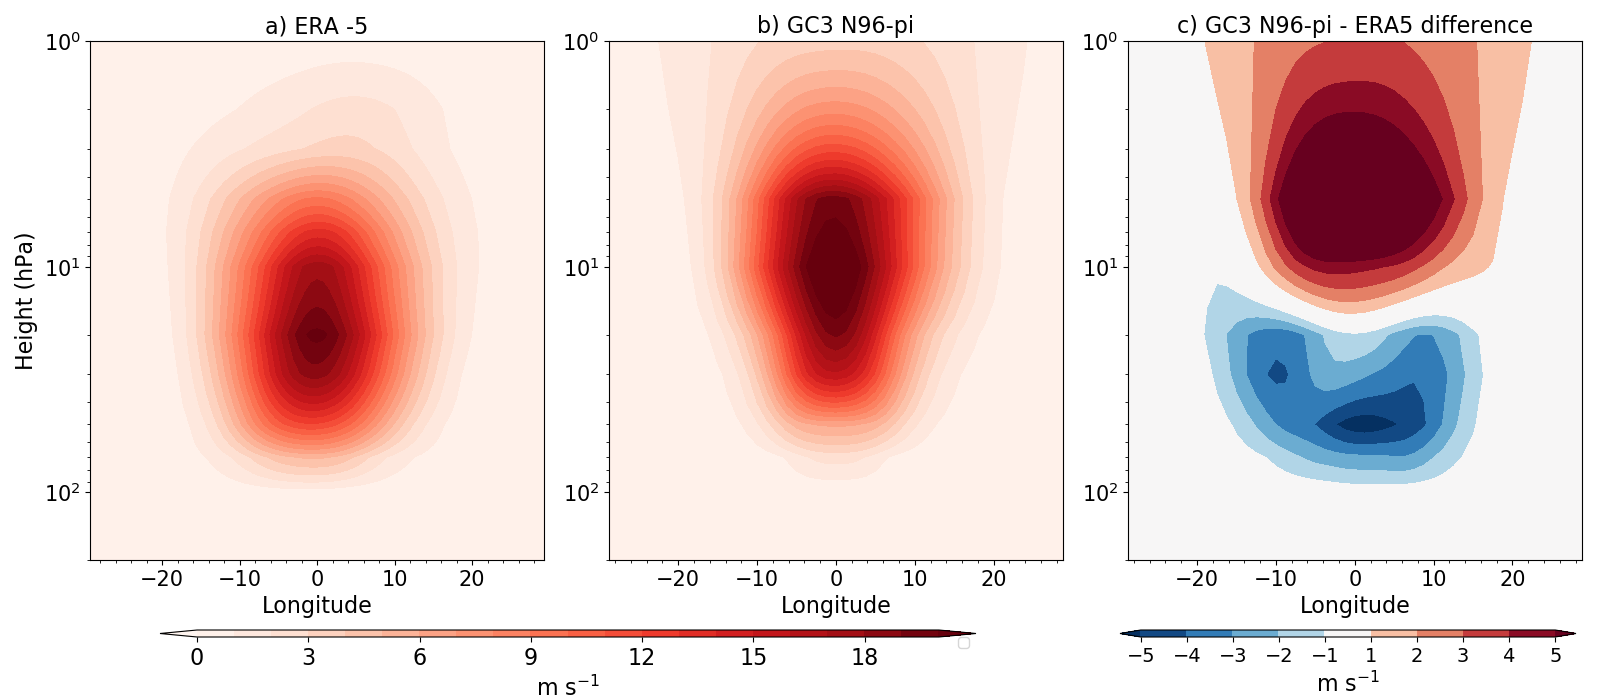
\includegraphics[width=\linewidth]{figures/qboamplitude.png}
\caption[QBO amplitude bias]{Latitude-pressure plot of the amplitude [m s$^{-1}$] of the QBO \added{for (a) ERA5 and (b) GC3 N96-pi. (c) The difference in amplitude between the (b) model and  reanalysis.} Obtained from the zonal mean zonal wind fourier spectrum magnitude within the QBO periods, as in \cite{schenzinger2017}. }
\label{fig:qboamplitude}
\end{figure} 


The physical mechanisms through which the QBO could influence tropical surface climate are also not well understood (see section \ref{sq:trop_qbo}). The influence of the QBO over the temperature and vertical wind shear near the tropopause layer \citep{tegtmeier2020b,martin2021variability} has been hypothesized to affect convection through several mechanisms \citep{haynes2021influence}.
Early studies \citep{gray1984,collimore2003} suggest that changes caused by the QBO to the vertical wind shear or static stability in the upper-troposphere lower-stratosphere (UTLS) region  modify the depth of convection at equatorial latitudes. However, other studies suggest that the surface impact of the QBO may be a function of both the UTLS temperature changes and the tropospheric convective forcing \citep{nie2015}.

The leading hypothesis to explain an impact from the QBO on tropical deep convection suggests that changes to the  UTLS static stability, caused by the QBO residual circulation, modifies the strength of convection  \citep{collimore2003,liess2012,nie2015,yamazaki2020tropospheric}. 
However, most of the existing climate models underestimate the amplitude of the QBO in the lowermost stratosphere (Figure \ref{fig:qboamplitude}) and by consequence the variability of the UTLS static stability associated with the QBO is lower in state-of-the-art GCMs \citep{schenzinger2017,richter2020,bushell2020}. 
  For example, the observed relationships between the QBO and the MJO have not been found in GCMs \citep{lee2018,kim2020} and one reason for these results may be the underestimation of the UTLS temperature variability associated with the QBO in current GCMs.
  
  %In addition,  only a relatively small number of studies have analysed tropical QBO teleconnections in a GCM, specifically in CMIP5/CMIP6 models \citep{serva2021}, as most CMIP analyses focus on the polar and subtropical routes of QBO influence \citep{richter2020,anstey2021}.
   The stratospheric biases in GCMs, such as the weaker amplitude of the QBO in the lower stratosphere, have led several studies to perform experiments in which the model stratosphere is relaxed towards an observed or idealized  state, more commonly known as nudging \citep[e.g.][]{garfinkel2011,lee2018,gray2020,richter2020,martin2021}. 
The nudging technique has proven useful because the relaxation can remove biases, identify causal pathways and test specific hypotheses regarding mechanisms \citep{gray2020,martin2021,haynes2021influence}. In particular, the nudging technique has been suggested as a potential tool to better understand observed relationships between the tropics and the QBO \citep{lee2018,martin2021}.

In short, there is a lack of robust evidence for QBO surface impacts in the tropics, due to the limited observational record and the relatively scarce modelling evidence of QBO, particularly with state-of-the-art GCMs. 
 The Met Office Hadley Centre (MOHC) Unified Model (UM) extends to the mesosphere and includes a self-generated QBO via a non-orographic gravity wave scheme that compares well to observations, except for the weak amplitude bias in the lower stratosphere \citep{richter2020}. Moreover, nudging has been succesfully applied to this model in previous studies \citep{telford2008description,gray2020}. For these reasons, this chapter uses the UM to investigate whether there are any surface impacts in the tropics associated with the QBO and what mechanisms may be at play in the observed stratospheric-tropospheric coupling.



This chapter first investigates whether there are any robust connections between the QBO and the tropical troposphere using the pre-industrial control simulations of the MOHC from CMIP6.  This analysis benefits from the extremely long simulations that can provide improved estimates of statistical significance when compared with the relatively short observational datasets. The first part will demonstrate robust links between the QBO and several features of tropical climate but no conclusive statement can be made on the direction of causality using these simulations. For that reason, nudging experiments feature in the second part of the chapter. Atmosphere-only and coupled ocean-atmosphere model simulations are analysed to evaluate the effect of improving the biases of the QBO amplitude on the surface response. Specifically, these experiments test the UTLS static stability hypothesis, so that stronger effects would be expected in a model with a stronger UTLS temperature variability associated with the QBO compared to a model with a weaker UTLS static stability variability.

The methodology and data used in this chapter are described in section \ref{sq:qbo_methoddata}, including the details on the nudging experimental setup. Then, the QBO impacts diagnosed in the CMIP6 experiments are presented in section \ref{sq:cmip6_qbo}. Section \ref{sq:nudging} examines the results from the nudging experiments. 
A discussion and conclusions are presented at the end of the chapter. % then the results from the CMIP6 experiments are analysed. The results from the targeted experiments are subsequently presented and finally the results are dicussed and conclusions are given from this chapter.
 % the relevance of this work
%   are ideal to investigate variability associated with the QBO because these experiments are very long integrations where external forcing is kept constant within the simulation and the 
%The remainder of this chapter is presented as follows. 
%First, the data and methods used are described, after which the results analysing the QBO impacts over the seasonal precipitation and surface temperatures  is given. 
%Then, a more detail investigation on the effects on the East Pacific and Atlantic ITCZs is presented and finally, the impacts over ENSO, the Indian Ocean and the Walker circulation are given. 
%A discussion is given at the end of the chapter.
% These simulations are examined first via composite analysis to investigate whether tropical convective phenomena such as the ITCZ and monsoon rainfall show any significant response to the state of the QBO. 





\section{Methods and data} \label{sq:qbo_methoddata}

The observational datasets and reanalysis (ERA5) used in this chapter are described in more detail in section \ref{sq:obsdata} and consist of the HadSST3 dataset for SST, GPCP and GPCC for precipitation and ERA5 for the rest of the diagnostics that include the zonal and meridional winds, air temperature, etc.

\subsection{CMIP6 data}
In section \ref{sq:cmip6_qbo}, three pi-control experiments are analysed: HadGEM3 GC3.1 at N96 and N216 horizontal resolutions (hereafter referred to as GC3 N96-pi and GC3 N216-pi) and UKESM at N96 horizontal resolution (hereafter referred to as UKESM N96-pi). The N96 and N216 atmospheric resolution is 1.875$^\circ$x1.25$^\circ$ and 0.83$^\circ$x 0.56$^\circ$, respectively whereas the oceanic resolutions are 1$^\circ$ (ORCA1) and 0.25$^\circ$  (ORCA025), respectively. The full 500 years available of the GC3 N216-pi simulation are used and although more data exists for UKESM-pi and GC3 N96-pi, we use 500-yrs of these simulations as well for consistency. 
The three simulations chosen use the same model setup, with constant year 1850 forcing, but differ in their horizontal resolution or the treatment of aerosol-chemistry processes and land-surface interactions (see section \ref{sq:modeldata}). 
 The CMIP6 version of the model model extends to the lower mesosphere and includes a self-generated QBO via a non-orographic gravity wave scheme that compares well with the observed QBO \citep{richter2020}. 

Pre-industrial control experiments are ideal for the purpose of examining the mechanisms of internal variability of a model because external forcing is kept constant throughout the usually long integrations (e.g. in CMIP6 these experiments are at least 500 years long). For these reasons, multiple studies have used this type of experiments to investigate teleconnections and variability on multiple time-scales isolated from the influence of external forcing \citep[see e.g.][]{watanabe2012uncertainty,zanchettin2014,palmer2014internal,menary2018,dimdore2021,villamayor2021causes}. For the purposes of this chapter, the model variability associated with the QBO which samples several states of decadal variability are compared against the observed variability associated with the QBO. 

The majority of the diagnostics in section \ref{sq:cmip6_qbo} are shown for the higher resolution GC3 N216-pi simulation and comparisons with the other two simulations are noted where appropriate. The equatorial climate of GC3 N216-pi  captures tropical dynamical processes and tropical mean and extreme precipitation reasonably well relative to lower-resolution configurations \citep{garciafranco2020,abdelmoaty2021biases}. This configuration has been top ranked amongst all CMIP5/CMIP6 models in metrics such as the seasonal-phase locking and amplitude of ENSO \citep{menary2018,richter2020overview,liu2021enso}, extreme precipitation \citep{abdelmoaty2021biases} and the annual cycle of equatorial Atlantic SSTs and low-level winds \citep{richter2020overview}. 
  The HadGEM model has also been historically top ranked in the representing the stratosphere and the QBO \citep{schenzinger2017,richter2020}.
  However, several biases are notable in this model, particularly in tropospheric dynamical features such as the southward bias of the Atlantic ITCZ linked to the dry Amazon bias and too strong precipitation rates over the East Pacific ITCZ \citep{garciafranco2020}.


\subsection{Indices}
\label{sq:indices}

For the QBO, the monthly-mean equatorially averaged [5$^\circ$S-5$^\circ$N] zonal mean zonal wind at 70 hPa is used  and each phase of the QBO is defined using the threshold of 2 m s$^{-1}$ \citep{garfinkel2010}, so the westerly phase (QBOW) is defined for months with an index value above 2 m s$^{-1}$ and the easterly phase (QBOE) for index values below -2 m s$^{-1}$. For ENSO, the EN3.4 SST index is used, with a running-mean of 5 months and a threshold of $\pm$0.5 K used to define positive or negative events. Neutral months are defined where the running-mean of EN3.4 index is smaller than $\pm$0.5 K.

The amplitude and descent rates of the QBO are calculated using the deseasonalized zonal mean equatorially averaged in equatorial latitudes for all levels. 
The amplitude ($A$) of the QBO is defined using the first and second principal components (PCs)  empirical orthogonal function (EOF) decomposition of the 10-70 hPa wind time-series \citep{serva2020} as $A=\sqrt{PC1^2+PC2^2}$.
The descent rates are calculated following \cite{schenzinger2017} for descending westerly and easterly phases individually by finding the level of the zero wind line ($u=0$) for each month and computing the difference between consecutive months.
These definitions of the amplitude and descent rates were chosen to evaluate the influence of ENSO on the whole profile of the QBO and not just one single level. 

An index for the Indian Ocean Dipole (IOD) was also required and this chapter uses a convective precipitation index of the zonal gradient in the Indian Ocean (convective IOD Index), defined as the difference of the deseasonalized area-averaged convective precipitation between the western [50-70$^\circ$E] and eastern [80-100$^\circ$E] equatorial [10$^\circ$S-10$^\circ$N] Indian Ocean, which is in a similar region as the standard SST IOD index \citep{wang2014iod}. 
This convective precipitation index is used to define IOD events with a 1 standard deviation threshold to define positive and negative events. 

\subsection{Analysis techniques}
\label{sq:analysis}

Composite analysis is the primary technique used in the study. For each month the QBO phase (QBO-E or QBO-W) and the  ENSO phase (El Niño, La Niña or neutral ENSO phase) was determined as described above. Annual-mean and seasonal-mean composites were derived by computing weighted averages to account for differences in the counts of each month, i.e, to avoid a possible aliasing with the seasonal cycle. This means the composites were derived by weighting each monthly-mean by its size and then computing the seasonal or annual-mean average so that all months contribute equally and there is no seasonal effect due to, e.g., QBO or ENSO phase-locking.

The length of the pre-industrial control experiments is such that the number of total El Niño and La Niña months for GC3 N216-pi were over 1000 months in the entire simulation for each phase, and over 1500 months for each QBO phase. Moreover, El Niño months found under QBOW were 376 and 284 under QBOE, whereas in the observed 1979-2018 period, 62 QBOW El Niño months and 36 QBOW El Niño months were diagnosed.

Linear regression analysis has proven useful to understand the effect of one or more aspects of the climate over a region or a time-series, and was used to investigate the surface impacts of the QBO in observations by \cite{gray2018}. 
A simple linear regression model can be written as:

\begin{equation}
Y(t)=X_0+X_i(t)\beta_i + \epsilon,
\end{equation}
\noindent where $Y$ is the measured or dependent variable, $X_0$ is a constant coefficient, $\beta_i$ is the regression coefficient between $X_i$ and $Y$ and $\epsilon$ represents random error or a residual.  In all cases, the models solved using an ordinary least-squares (OLS) method.
A multivariate regression model can be used to study the joint effect of two or more predictors over a variable ($Y$) such that the model can be written as:
\begin{equation}
Y(t)=X_0+\sum_j^NX_j(t)\beta_j+\epsilon
\end{equation}
\noindent where $X_j(t)$ is any predictor with an associated regression coefficient $\beta_j$. The multivariate regression will be used to separate the linear influence of the QBO and ENSO in section \ref{sq:cmip6_qbo}.
As in previous studies \citep{gray2018,misios2019slowdown}, the regression coefficient can be rescaled to evaluate the total effect that a predictor ($X_j$) can have on the variance of the measured variable ($Y$) using the standard deviation ($\sigma_j$) and the maximum ($X_{j,max}$) and minimum ($X_{j_min}$) values of $X_j$ so that the rescaled coefficient $\beta_j^\prime$ can be written as:

\begin{equation}
\beta_j^\prime=\beta_j\frac{X_{j,max}-X_{j,min}}{\sigma_j}.
\end{equation}

%The regression analysis will be used in the following sections to s

\subsection{Nudging experimental setup}\label{nudg_setup}

This section describes the experimental setup for the nudging experiments. 
The GC3.1 configuration of the UM model is used (model version 11.4), using an atmospheric horizontal resolution of N96 (corresponding to the low-resolution version of the MOHC CMIP6 simulations). 
Both atmosphere-only and ocean-atmosphere coupled experiments were conducted for the period 1981-2015, using a present-day climate setup where all external forcings, including greenhouse gas and aerosol emissions, are set constant to those of the year 2000. %, so there is no variation in, e.g., greenhouse gases within these simulations.

Nudging refers to the relaxation of a model variable towards a specified state which can be from reanalysis, observations or idealized states \citep{gray2020,martin2021}. In the UM setup, three variables can be relaxed, air temperature ($T$) and the zonal ($u$) and meridional ($v$) components of the wind. The relaxation is applied at each grid-point, in contrast to the setup in other models \citep[e.g.][]{martin2021} where the relaxation is performed in a zonal-mean sense. Specifically, the UM uses a Newtonian relaxation technique \citep{telford2008description,gray2020} which sets the field to be relaxed ($F$) at each time-step through the following equation:  


\begin{equation}
\Delta F=G\Delta t (F_{ndg}-F_{model}),
\end{equation}

\noindent where $\Delta F$ is the discrete change of $F$ at each time-step, $G$ is the relaxation parameter, $\Delta t$ is the time-step size, $F_{ndg}$ is the value of the field from the nudging data and $F_{model}$ is the model value of the field at the last time-step \citep{telford2008description}.

The relaxation parameter $G$ sets the strength of the relaxation and is linked with the relaxation timescale ($\tau$) by $G=1/\tau$. In the UM model, the relaxation timescale is given by the temporal resolution of the nudging data, which is 6-h \citep{telford2008description,gray2020}, so that $G=\frac{1}{6}$ h$^{-1}$. This relaxation parameter has been shown to be sufficiently strong to constraint the stratospheric state of the model \citep{gray2020} and so the same parameter was used for the simulations of this chapter. 

Furthermore, the nudging can be performed between specified vertical levels and in selected latitude/longitude regions with \textit{tapering}. The tapering refers to a linear interpolation between the maximum $G$ and zero nudging ($G=0$). 
For example, a tapering of 4 vertical levels was applied in our simulations which means that there was a linearly increasing $G$ from a bottom level with no nudging to the level where the specified $G$ is  implemented; the same linear interpolation works for latitudinal tapering.

%The UM version 11.4 was used with atmospheric resolution of N96  (1.875$^\circ$x1.25$^\circ$) in all the experiments, external forcing is seasonally varying but constant to represent year-2000 forcing conditions, including, e.g., aerosol emissions.
The experimental design chosen relaxes the zonal wind ($u$) in the model levels corresponding to 90 hPa to 4 hPa, with a tapering of 4 levels, which means that full nudging was only working from 70 hPa to 10 hPa. The nudging was done at all longitudes in the latitude band of 10$^\circ$S-10$^\circ$N with a latitudinal tapering of 10 degrees on both sides, which means that at 20$^\circ$N the relaxation parameter was 0.
The experimental setup aims to reasonably simulate the observed variability of the zonal wind leaving the meridional component of the wind and the temperature to respond freely within the model. 

\begin{table}[t!]
\caption{Experimental setup indicating the model configuration, the period, ensemble members (Ens.) acronym and relaxation details.}
\begin{tabular}{p{3.2cm}|p{2.cm}|p{1.35cm}|p{3cm}|p{4.85cm}} \label{tab:nudg_exps}
Setup           & Period    & Ens.& Name            & Nudging                                          \\ \hline \hline
Atmosphere-only & 1981-2015 & 3                & AMIP            & ERA5. U-only 90 hPa                              \\
Atmosphere-only & 1981-2015 & 2                & AMIP-Control    & No                                               \\
Atmosphere-only & 1981-2015 & 3                & AMIP-Shifted    & ERA5. U-only, 90 hPa. Relaxation shifted -1 year. \\
Coupled         & 1981-2015 & 6                & Coupled Nudged     & ERA5. U-only 90 hPa.                             \\
Coupled         & 1981-2015 & 2                & Coupled Control & No.                                             
\end{tabular}
\end{table}

Atmosphere-only and coupled ocean-atmosphere simulations were performed with this nudging setup, with corresponding control simulations in which there was no relaxation of any kind (Table \ref{tab:nudg_exps}). The atmosphere-only (AMIP) experiments were run by prescribing the CMIP6 SST dataset used for AMIP experiments, note the surface boundary SSTs are used at all latitudes. The coupled experiments use an oceanic resolution of 0.25$^\circ$ (ORCA025) using the NEMO model \citep{storkey2018}. Each ensemble member was initialized from different ocean/atmosphere initial conditions in order to decrease the role that internal variability may have on these simulations. Specifically, the coupled ocean-atmosphere configuration was initialized oceanic conditions of a long integration of the same model configuration that were found 10 years apart from each other in the spin-up simulation.
For each of the configurations several ensemble members were launched (see Table \ref{tab:nudg_exps}). 


Note that the coupled experiments differ only slightly from the setup used in the CMIP6 piControl experiments, with the atmospheric resolution matching the resolution of GC3 N96-pi (1.875$^\circ$x1.25$^\circ$) and the oceanic resolution being the same as GC3 N216-pi (0.25$^\circ$). The forcing is constant in both types of runs, except that in the piControl experiments, the forcing represents conditions of the year 1850 and in these experiments the forcing is for the year 2000. 



In addition to the nudged and control coupled and AMIP experiments, we performed another type of atmosphere-only experiment. In the normal AMIP Nudged experiment, the SST driving data corresponds to the same year as the imposed zonal wind in the equatorial stratosphere that was observed in the real-world. To explore possible feedback processes between QBO winds and the SSTs, we performed an AMIP Shifted experiment, where the nudging data was shifted with a -1 year lag from the SSTs. In this experiment, e.g., the model year 1997 was run using 1997 SSTs but zonal winds in the stratosphere corresponding to 1996 of ERA5. In this way we have minimised any in-phase relationship between the QBO phase and the SSTs. An alternative approach would be to \textit{shuffle} the SSTs so that each year is run with randomly selected SSTs. However, since we are performing multi-year simulations shuffling has associated issues of how to join the randomly-selected SSTs at the year-boundary to form a coherent multi-year SST time-series. To avoid this issue we decided to simply shift the SSTs by one year so the QBO phase and SSTs were not aligned.

  
\section{Teleconnections in the pre-industrial control experiments}\label{sq:cmip6_qbo}

The tropical precipitation response to the QBO phase is analysed in both observations and model simulations, first in the annual-mean and then by season (section \ref{qbo7_pr}).  The potential for aliasing with the ENSO signal is investigated (section \ref{qbo7_enso}) and QBO-ENSO interactions are further explored (section \ref{sq:iod_enso}), as well as QBO interactions with the Indian Ocean dipole (IOD). Finally, interactions between the QBO and the ITCZ, monsoons and the Walker circulation are identified and discussed in \ref{sq:circ}. 

\begin{figure}[t!]
\centering
 %\noindent
 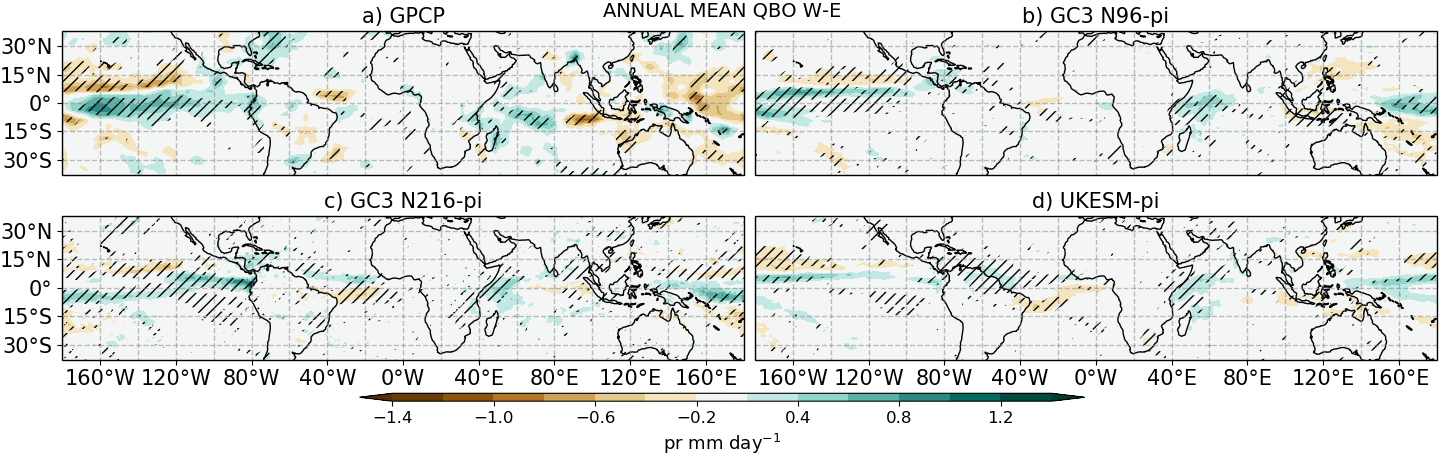
\includegraphics[width=\linewidth]{figures/piprclimqbowqboe.png}
\caption[Annual mean precipitation composite difference QBO W-E ]{ QBO-W minus QBO-E composite differences in annual-mean precipitation from (a) GPCP, (b) GC3 N96-pi, (c) GC3 N216-pi and (d) UKESM-pi. Hatching denotes statistically significant differences at the 95\% confidence level using a bootstrapping with replacement test. }
\label{fig:qboclim}
\end{figure}


\subsection{Precipitation} \label{qbo7_pr}

QBO composite differences in annual mean precipitation (QBO-W minus QBO-E) are shown in Figure \ref{fig:qboclim} from the gridded GPCP observational dataset and from all three model simulations. In the observations the QBO signals are largest and statistically significant in the tropical Pacific, equatorial Atlantic and Indian Oceans, in good agreement with previous analyses \citep{liess2012,gray2018}. The three simulations agree reasonably well with the GPCP distributions and amplitudes, particularly in the Pacific and Indian Oceans. Positive differences of up to 1.2 mm day$^{-1}$ are found in the equatorial Central Pacific and the Indian Ocean and negative differences of up to 0.6 mm day$^{-1}$ in the off-equatorial North Pacific, although the differences are smaller in the simulations than observed. 

In the tropical Atlantic, however, there is an indication of a weak but significant signal in the observations near the ITCZ but the models show a signal of the opposite sign in this region (or the absence of a signal in the case of GC3 N96-pi). This disagreement with observations may be due to the biased southward position of the Atlantic ITCZ in the model which is more pronounced in DJF \citep{garciafranco2020}.

\begin{figure}[t!]
\centering
 %\noindent
 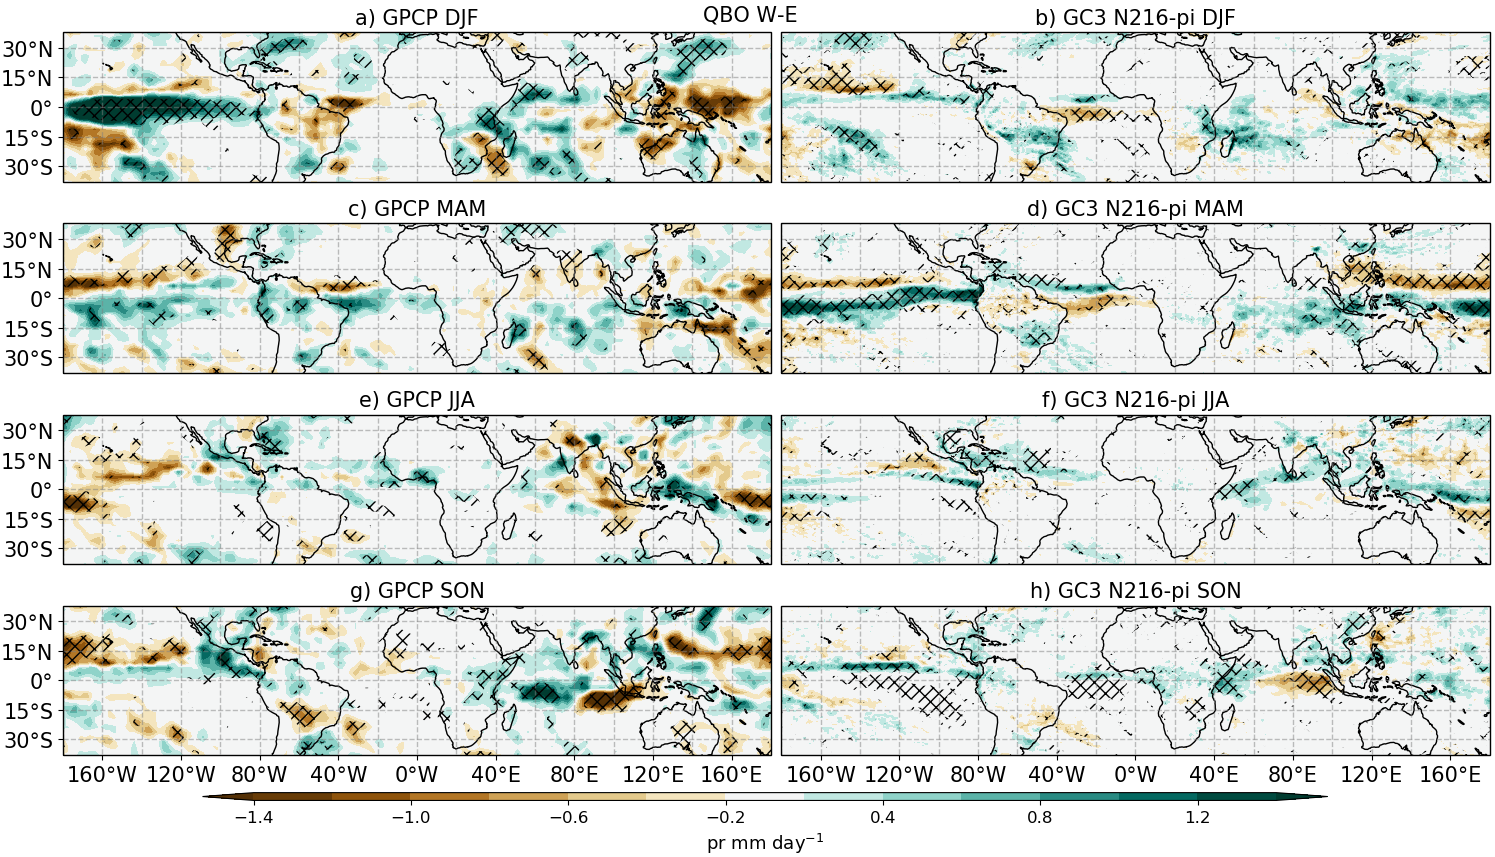
\includegraphics[width=\linewidth]{figures/paperprqbowqboe.png}
\caption[Seasonal mean precipitation composite difference QBO W-E ]{ As in Figure \ref{fig:qboclim}, but showing seasonal-mean QBO composite  from (left) GPCP and (right) GC3 N216-pi for DJF, MAM, JJA and SON from top to bottom. }
\label{fig:qbodjf}
\end{figure}

The QBO signal in precipitation is found to be strongly dependent on the seasonal cycle in both models and observations. Figure \ref{fig:qbodjf} shows a comparison of the GPCP dataset and GC3 N216-pi for individual seasons. The positive equatorial Pacific signal in the GPCP dataset, which resembles an El Niño anomaly, is particularly strong and statistically significant in December-January-February (DJF) (Fig. \ref{fig:qbodjf}a). A similar pattern is present in both March-April-May (MAM) (Figure \ref{fig:qbodjf}c) but with no statistical significance. In GC3 N216-pi the QBO signal in the Pacific is significant in all seasons, likely due to the greater number of years in the ensembles, although it is shifted slightly compared to GPCP and is strongest in MAM (Fig. \ref{fig:qbodjf}c).   

In the Atlantic, the QBO signal in the ITCZ region is more clearly evident in the individual seasons. In DJF there is reasonable similarity between the model and observations but by MAM the opposite sign of the model compared to GPCP becomes evident, even though the ITCZ bias in the model is stronger in DJF than in MAM \citep{garciafranco2020}. In addition, all models and GPCP indicate that the Caribbean Sea is wetter in JJA during QBO-W than in QBO-E (see Fig. \ref{fig:qbodjf}). In the Indian Ocean, the observations and all models show relatively large and significant differences in SON, (Fig. \ref{fig:qbodjf}e-f), characterized by a dipole of wet anomalies to the west and dry anomalies to the east. The dipole anomalies suggest a possible QBO influence on the IOD, which is characterized by a zonal gradient of SSTs and convective activity in the Indian Ocean that is specially prominent in SON \citep{saji1999iod,deser2010sea,mckenna2020iod}. This possibility is explored further in section \ref{sq:iod_enso} below.  

In summary, the GPCP precipitation composite differences, characterized by a zonally asymmetric QBO signal that is primarily found over the oceans, are consistent with previous analyses \citep{liess2012,gray2018}, and the simulated QBO response patterns are in good agreement with the observations. This good agreement, together with the length of the model simulations (500 years) compared with the available observations, suggests that analysis of the modelled QBO signals may help to understand the mechanisms that give rise to the surface response in the QBO. However, the QBO signals from both model and observational analyses are very similar to well-known patterns for ENSO and the IOD. Previous observational studies have also shown a higher frequency of El Niño events during QBOW and of La Niña during QBOE in observations since 1979 \citep{taguchi2010,liess2012}, although the observational record is short so there is much statistical uncertainty. This potential for aliasing of the QBO and ENSO signals is investigated in the next section.

\begin{figure}[t!]
\centering
 %\noindent
 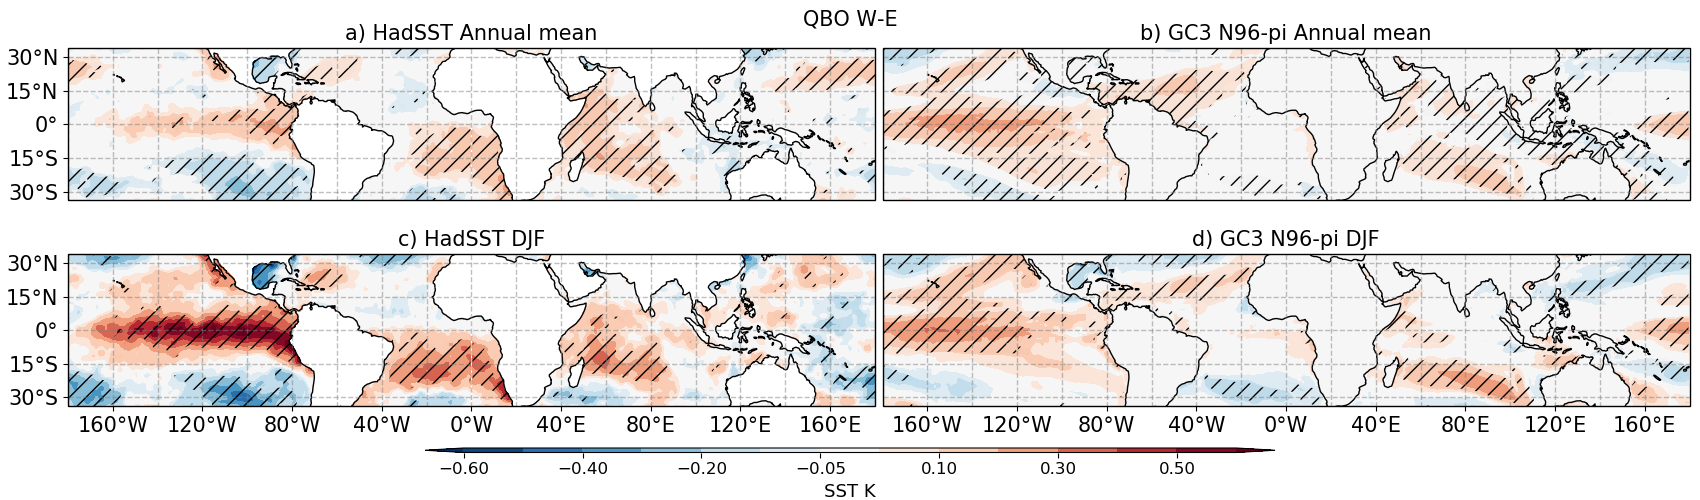
\includegraphics[width=\linewidth]{figures/papersstqbowqboe.png}
\caption[Annual mean SST difference QBO W-E under different QBO phases.]{ As in Figure \ref{fig:qbodjf} but for seasonal-mean sea surface temperatures from (left) the HadSST dataset and (right) GC3 N216-pi simulation.}
\label{fig:sstclim}
\end{figure}

\subsection{Potential aliasing of QBO and ENSO signals} \label{qbo7_enso}

To further explore the QBO signal and its interaction with ENSO, Figure \ref{fig:sstclim} shows the QBO signal in SSTs. The QBOW minus QBOE composite differences are shown for individual seasons from the HadSST dataset and the GC3 N216-pi model simulation. The SST signals are consistent with the precipitation signals. Both model and observational datasets show significant positive SST responses in the equatorial Pacific that are similar to El Niño patterns. In the HadSST dataset the Pacific response is strongest in DJF and resembles an East Pacific (or ’standard’) El Niño, whereas the simulated anomalies in DJF are weaker and look more like a central Pacific El Niño \citep{capotondi2015}. 

\begin{figure}[t!]
\centering
 %\noindent
 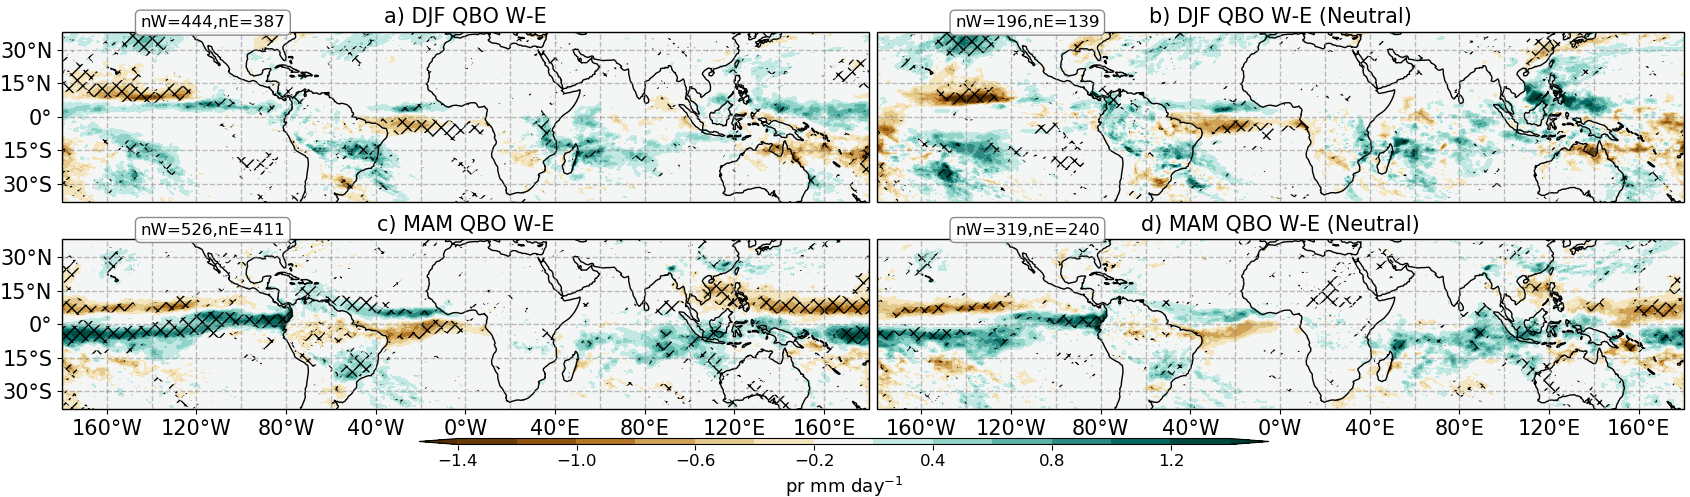
\includegraphics[width=\linewidth]{figures/qbonnpr.png}
\caption[Precipitation response to QBO W-E for GC3 N216-pi under different QBO phases.]{  Composite QBO W-E differences of total precipitation in GC3 N216-pi in (a, b) DJF and (c, d) MAM for (a, c) all the events and (b, d) Neutral ENSO conditions only. The sample size of each composite is noted in the top left corner of each panel. Statistically significant differences to the 99\% confidence level are shown through the hatching. }
\label{fig:qbonn}
\end{figure}

In GC3 N216-pi, the largest differences are observed in MAM in the easternmost Pacific Ocean and thus more closely resembles the observed DJF response pattern. In the South Atlantic the model shows a region weak, insignificant cooling in DJF (Figure \ref{fig:sstclim}d), in contrast to the statistical significant warming signal in HadSST (Figures \ref{fig:sstclim}a,c). In the northern tropical Atlantic the model shows an year-long warming signal with stronger anomalies in MAM and JJA; this signal is present in HadSST but only found in JJA and SON and it is not significant (Fig. \ref{fig:sstclim}e, g). The simulated northern tropical Atlantic warm anomalies in DJF (Figure \ref{fig:sstclim}b) are accompanied by a warmer Caribbean Sea and a cooling of the Gulf of Mexico, warmer SSTs along the coast of California and a cooling of the central North Pacific, all of which resemble the impact of El Niño events and the positive phase of the Pacific North American (PNA) pattern \citep{deser2010sea,guo2017distinct,jimenezesteve2020}.  

As an initial investigation of the possibility of aliasing between the QBO and ENSO signals, Figures \ref{fig:qbonn}a,b shows the DJF QBOW minus QBOE composite differences of total precipitation from the GC3 N216-pi simulation using all years (as in figure \ref{fig:qbodjf}) compared with using only those years identified as ‘ENSO-neutral’. Although the sample size is substantially reduced in the latter (see figure for the number of months in each QBO composite) the sample size is nevertheless still large (>120 data points in each composite). The response patterns are similar in each plot, which suggests that the QBO signal is unlikely to be the result of a sampling bias that favours one particular phase of ENSO.  

\begin{figure}[t!]
\centering
 \noindent
 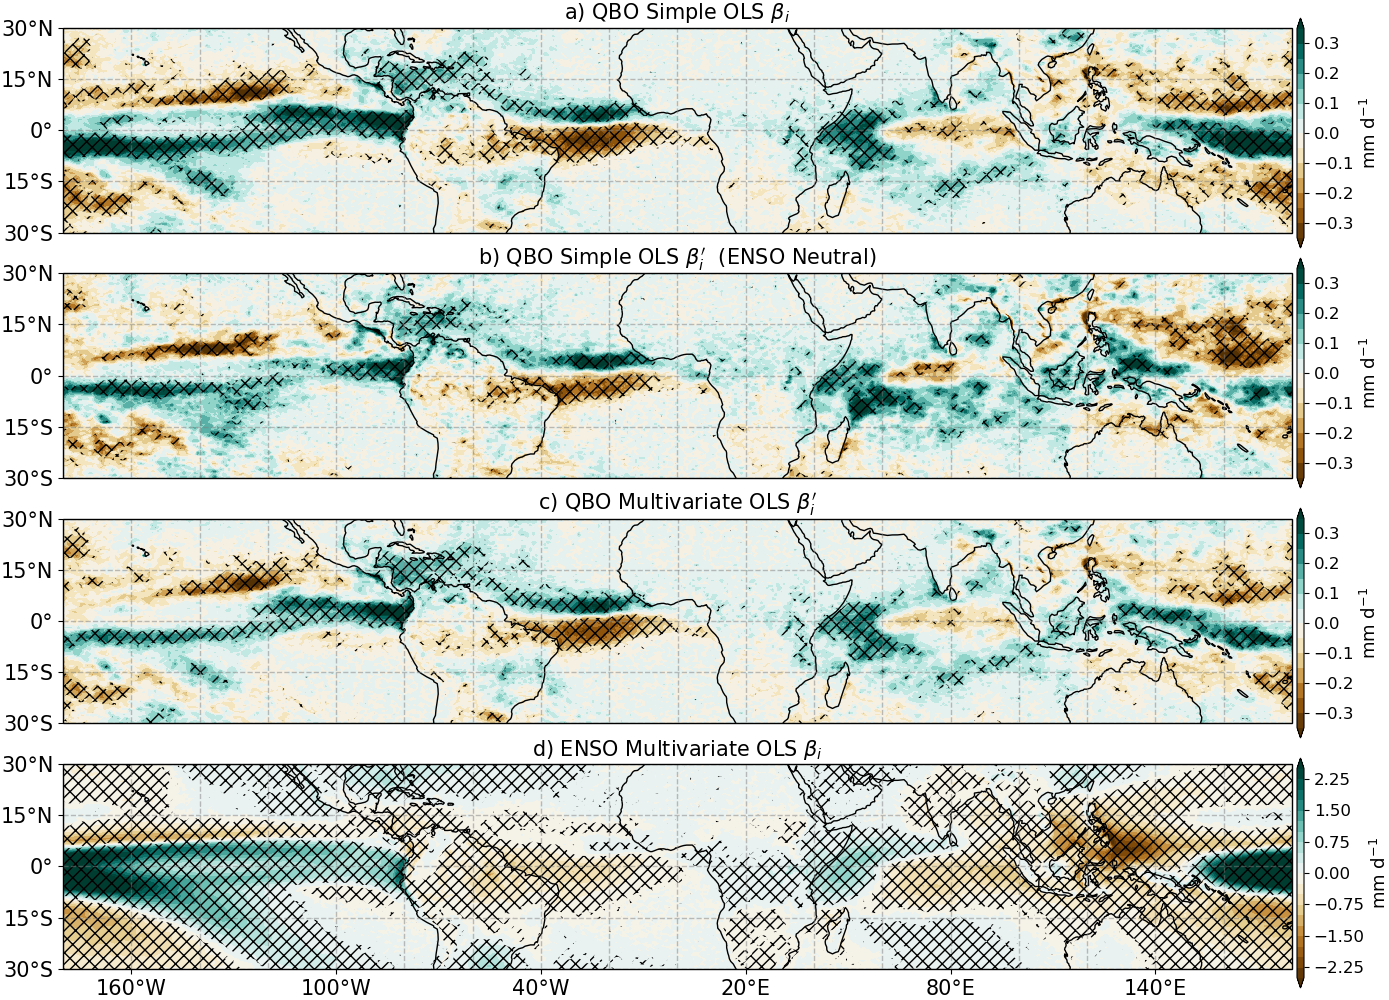
\includegraphics[width=\linewidth]{figures/regress_n216v2.png}
\caption[Convective precipitation regression analysis]{Annual-mean regression model results in GC3 N216-pi for convective precipitation. (a, b) Regression coefficients ($\beta_i$) from a simple ordinary least-squares (OLS) regression model with the QBO index for (a) all months and (b) ENSO-Neutral months only. (c, d) show the regression coefficients resulting from a multivariate regression model using the ENSO and QBO indices for the (c) QBO and (d) predictors. In all cases, the regression coefficients are rescaled by multiplying the regression coefficients with the ratio of maximum amplitude and standard deviation of the QBO or ENSO indices. }
\label{fig:enso_regress}
\end{figure}

An alternative approach to investigate the possibility of aliasing of the QBO/ENSO signals is to use a multi-linear regression technique (see section 2) in which the signal is analysed for both QBO and ENSO simultaneously. Here, we switch to analysing convective precipitation to better investigate the possible influence of the QBO on tropical deep convection.

Figures \ref{fig:enso_regress}a,b show results from a simple linear regression analysis of the monthly-averaged time-series of GC3 N216-pi total precipitation in which a single QBO index is employed. Figure \ref{fig:enso_regress}a includes all available years while Figure \ref{fig:enso_regress}b includes only neutral ENSO years. The results are very similar to the annual-mean composite differences in total precipitation (\ref{fig:qboclim}), with increased convective precipitation over the equatorial Pacific when the zonal winds at 70 hPa are positive. 

Figures  \ref{fig:enso_regress}c,d show the ENSO and QBO signals when the Nino3.4 index is included as well as the QBO index.  The ENSO response is clearly evident, highly statistically significant and compares well with the well-known patterns obtained from observations. The amplitude of the ENSO signal is also much larger than the QBO signal. Nevertheless, the QBO signal remains intact and all of the main features are still significant (Fig.  \ref{fig:enso_regress}c). For example, the positive regression coefficients that suggest a northward shift of the Atlantic ITCZ and the wetter Caribbean Sea and western Indian Ocean in the simple regression model are still found in the multivariate regression analysis.  

 
These results suggest that the modelled QBO signal in total precipitation does not arise due to a simple aliasing of the signal with ENSO. However, the multi-linear regression technique assumes that the QBO and ENSO indices are orthogonal and that their responses add together linearly. The similarity of the two responses indicate that this is clearly not the case and there is substantial interaction between the two phenomena. Nevertheless, the QBO signal remains even when only neutral-ENSO years are included in the analysis, suggesting that the QBO has a real influence on the surface precipitation.

\subsection{Interaction of the QBO with ENSO and IOD}
\label{sq:iod_enso}

\begin{figure}[t!]
\centering
 \noindent
 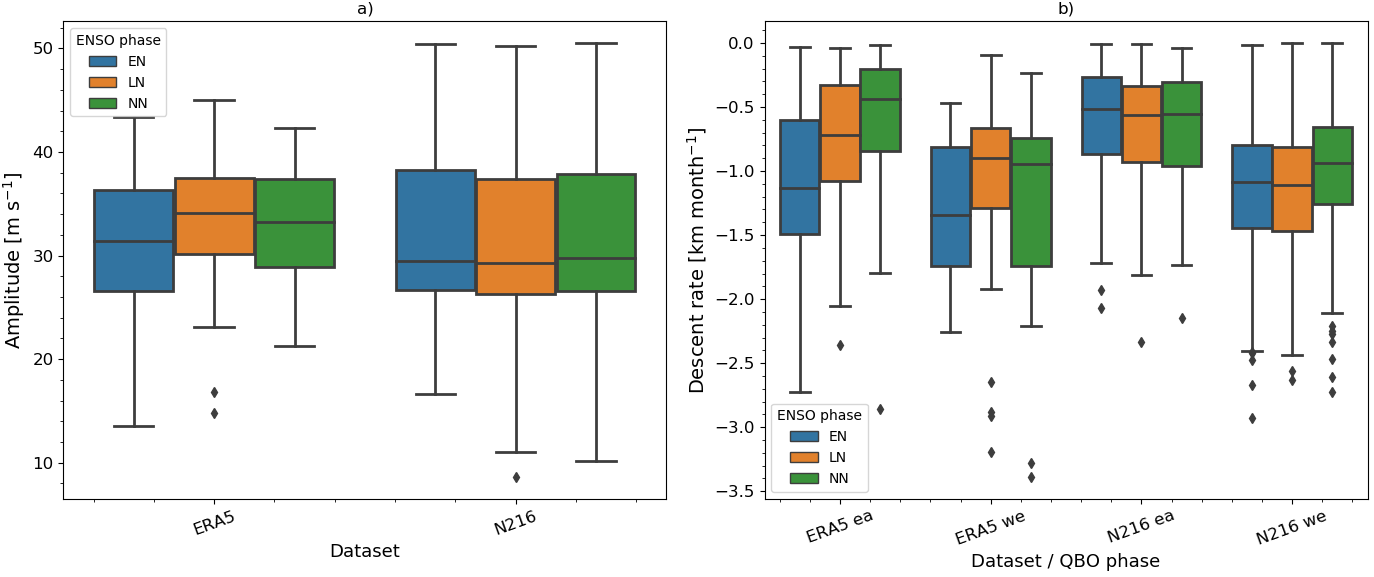
\includegraphics[width=\linewidth]{figures/scatter_qbom.png}
\caption[Scatter of relationship between QBO descent and amplitude and ENSO phase.]{Box plots of QBO (a) amplitude [m s$^{-1}$]  and (b) descent rate [km month$^{-1}$]  separated by dataset (ERA5 and GC3 N216-pi) and ENSO phase. NN stands for Neutral ENSO. In (b) descent rates are shown for both descending easterly (ea) and westerly (we) phases following \cite{schenzinger2017}. }
\label{fig:enso_on_qbo}
\end{figure}

To further explore the interaction of the QBO and ENSO, we first investigate whether aspects of the QBO are influenced by ENSO events. This relationship could be a real possibility since the intrinsic mechanism of the QBO involves tropical waves that are generated within the troposphere. \cite{schirber2015} found in a GCM that under El Niño conditions tropospheric wave activity increases and accelerates the downward propagation speed of the QBO westerly phase. However, the analysis by \cite{serva2020} shows that only models with high resolution can reproduce the observed ENSO effects on the QBO amplitude while several models show no impact of ENSO on the QBO.

For that reason, we analyse several characteristics of the QBO and their dependence on ENSO phase, namely the descent rate and the amplitude of the QBO (see the 'Methods and Data' section for details of how the QBO amplitude is defined). The results are summarised in Figure \ref{fig:enso_on_qbo} for the ERA5 reanalysis dataset (35 years; 1979 – 2014) and for the GC3 N216-pi simulation (500 years).  
In ERA5, the well-known faster descent rates during the westerly phase than in the easterly phase is clearly evident and agrees well with studies of longer datasets such as the Berlin radiosonde data \citep{schenzinger2017}. Also, the ERA5 QBO descent rates and the amplitude both depend on the phase of ENSO. A higher amplitude and slower descent rates are observed during La Niña phases and weaker amplitudes and faster descent rates during El Niño. 

In the model, the descent rates are also faster for the westerly than the easterly QBO phase, as observed, but the relationship between the QBO characteristics and ENSO is less clear. Neither the amplitudes nor descent rates of the QBO are significantly different between El Niño (EN) and La Niña (LN) phases. Interestingly, the only significant difference in the model is that descending westerlies are slower in Neutral ENSO months compared to EN or LN conditions, perhaps suggesting that tropical wave activity is increased in both ENSO phases compared with neutral years.  The model results therefore suggest that there is little influence of ENSO  on the descent rate and amplitude of the QBO in the GC3 N216-pi simulation. This finding of a null influence of ENSO on the QBO  agrees well with the results of \cite{serva2020} that examined these relationships in an older version of the HadGEM model. In summary, there is no evidence to suggest an influence of ENSO on the QBO in the model. 

\begin{table}[t!]
\caption{ENSO and IOD events frequency (month month$^{-1}$). For positive and negative events, for each mean value the error shown is the standard deviation of the probability density distribution (PDF) found by boostrapping with replacement. Results in \textbf{bold}  indicate that the event frequency PDF for QBOW is significantly different to QBOE to the 95\% confidence level according to the KS test.  }\label{t1}
\begin{center}
\begin{tabular}{cccccc}
\hline\hline
Dataset & QBO phase & El Niño & La Niña & IOD+ & IOD-  \\
\hline
GC3 N216-pi & W 	& \textbf{0.24$\pm$0.09} & \textbf{0.19$\pm$0.05} & \textbf{0.17$\pm$0.03}	 & \textbf{0.11$\pm$0.02} \\
GC3 N216-pi & E  & \textbf{0.21$\pm$0.07} & \textbf{0.26$\pm$0.07} & \textbf{0.12$\pm$0.03} 	 & \textbf{0.15$\pm$0.03}  \\
ERA5/HadSST & W & 0.28$\pm$0.01 & 0.27$\pm$0.02 & 0.17$\pm$0.01  &0.13$\pm$0.01 \\
ERA5/HadSST & E  & 0.17$\pm$0.02 & 0.27$\pm$0.03 &0.12$\pm$0.01 & 0.19$\pm$0.03 \\
\hline
\end{tabular}
\end{center}
\end{table}

The reversed possibility, that the QBO may somehow influence ENSO events is now examined. A higher frequency of EN events during QBOW and of LN during QBOE has previously been noted \citep{taguchi2010,liess2012} although the short observational record means that there is statistical uncertainty.  In Table \ref{t1} we document the frequency of ENSO events in each QBO phase from the ERA5 reanalysis dataset and from the GC3 N216-pi simulation. Probability density functions (PDFs) were constructed for the model data using 36-yr samples with replacement and a Kolmogorov–Smirnov (KS) test was used to evaluate if the PDFs of an event frequency (e.g. El Niño) were distinguishable for each phase of the QBO. 

The results show significant differences for each ENSO phase in GC3 N216-pi (and this is also the case for the GC3 N96-pi and UKESM-pi simulations, not shown). El Niño events are more frequent under QBOW conditions than under QBOE in both observations and model datasets.  La Niña events are equally frequent in both QBO phases in the HadSST dataset but in GC3 N216-pi they are more frequent under QBOE than under QBOW. 

\begin{figure}[t!]
\centering
 \noindent
 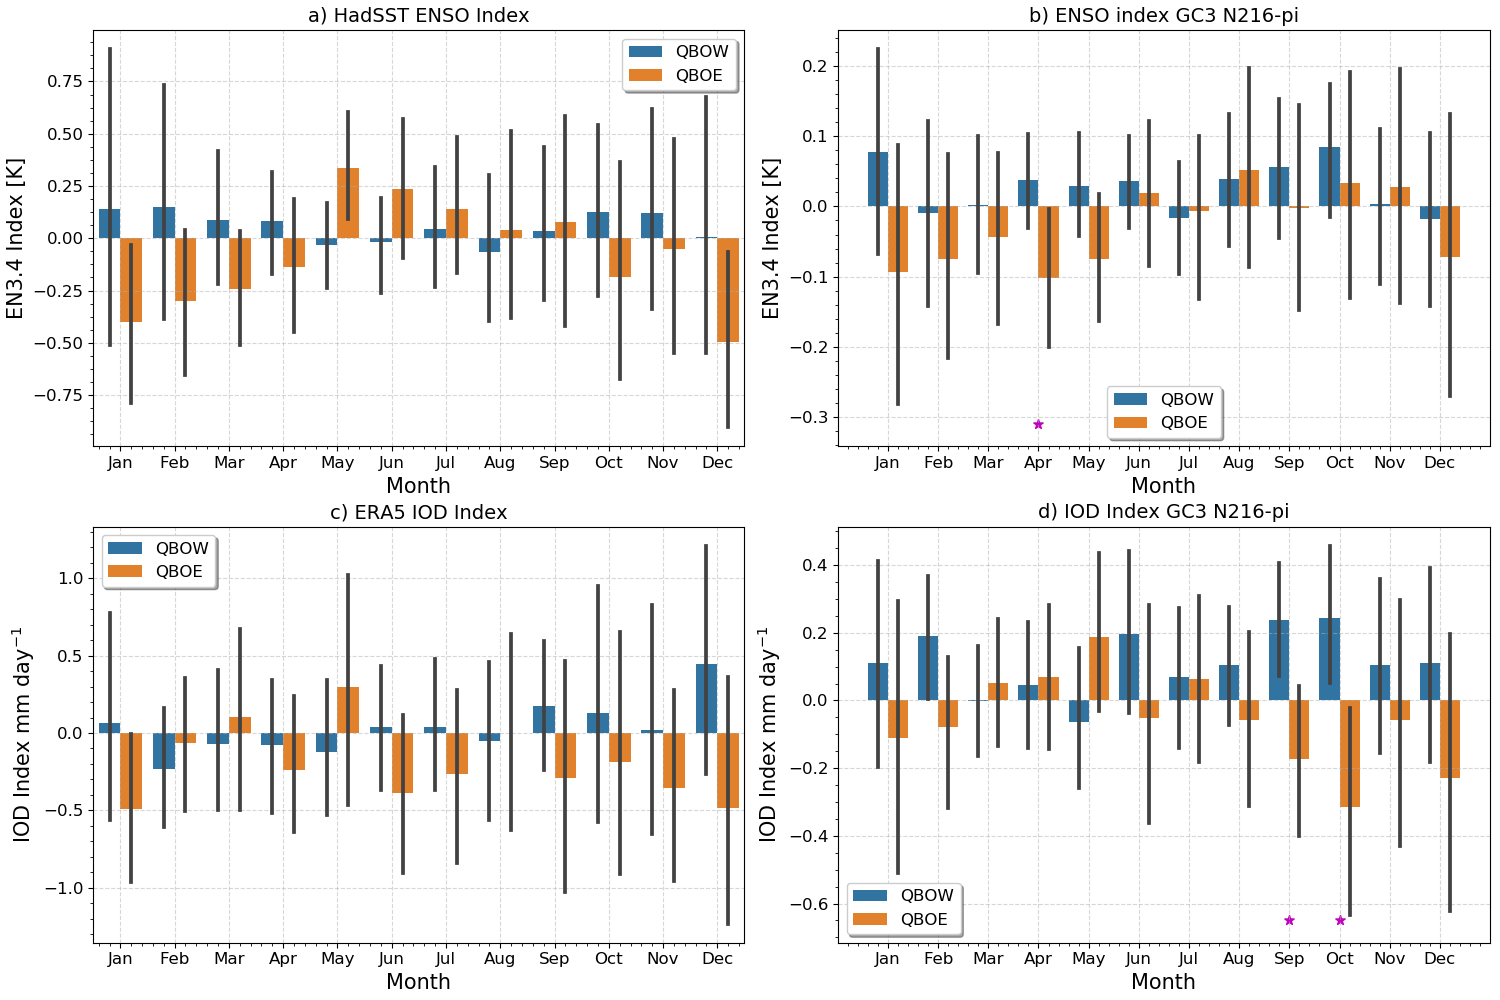
\includegraphics[width=\linewidth]{figures/iod_barplot.png}
\caption[IOD and ENSO frequency changes on QBO phase.]{ Monthly-mean (a-b) ENSO and (c-d) IOD-prc indices separated per QBO phase in (a, c) observations/reanalysis and (b, d) GC3 N216-pi. The error bars show the standard deviation of each index for each month and significant differences between QBO W and E months are highlighted with a $*$ at the bottom of each panel.  }
\label{fig:iod_barplot}
\end{figure}

Figure \ref{fig:iod_barplot}a,b shows the ENSO3.4 index amplitude and interannual standard deviation as a function of each month from the HadSST dataset and the GC3 N216-pi simulation, separated for each phase of the QBO. From this we can examine, for example, whether any QBOW minus QBOE differences in ENSO characteristics arise primarily from one QBO phase or the other (i.e. a non-linear response) or whether both phases contribute equally to the response difference.  There are significant QBO differences in EN3.4 SST in both the HadSST and GC3 N216-pi datasets. In particular, the mean ENSO indices are very frequently positive in QBOW and negative in QBOE months from September until January. In the model, the differences are largest from Feb-to-May (in good agreement with the results shown in Figure \ref{fig:qbodjf}).

  \begin{figure}[t!]
\centering
 %\noindent
 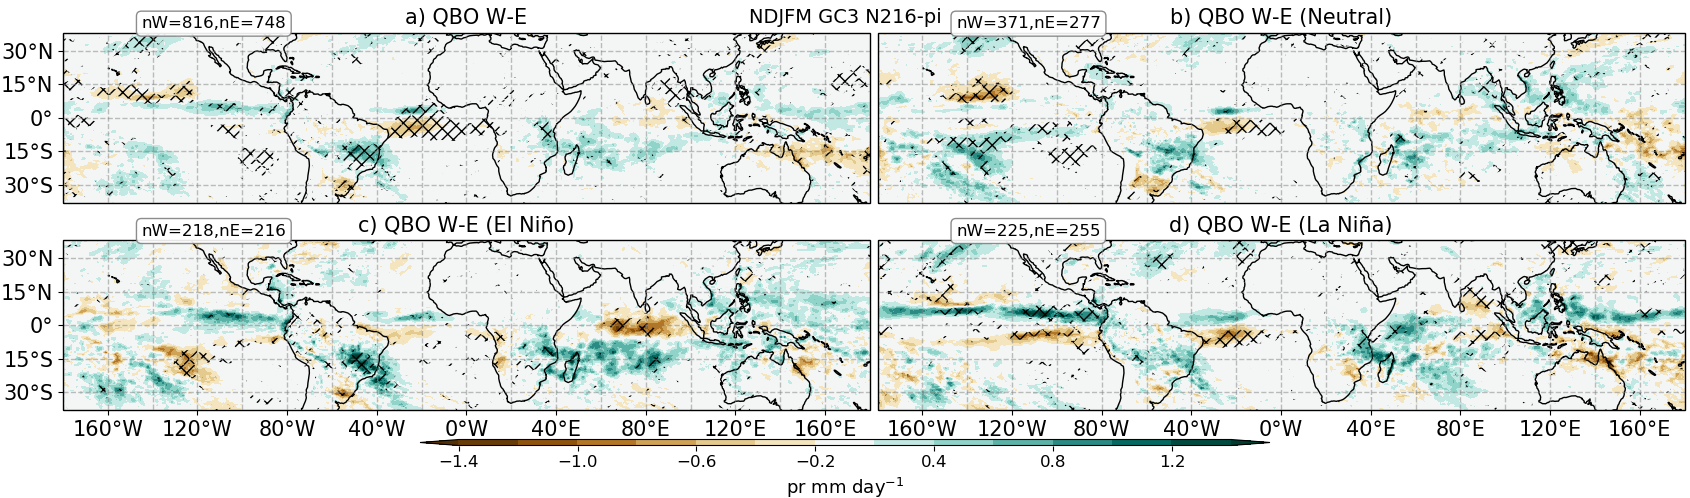
\includegraphics[width=\linewidth]{figures/ensoqboprwinter.png}
\caption[Precipitation response to QBO W-E for GC3 N216-pi under different QBO phases.]{  Composite QBO W-E precipitation differences of total precipitation in GC3 N216-pi in the peak ENSO season (NDJFM) for (a) all the events and (b) Neutral ENSO conditions only, (c) El Niño and (d) La Niña. The sample size of each composite is noted in the top left corner of each panel. Statistically significant differences to the 99\% confidence level are shown through the hatching. }
\label{fig:qboenso}
\end{figure}

Figure \ref{fig:iod_barplot} also suggests substantial non-linearities in the QBO-ENSO interactions, since the amplitude of the EN3.4 anomaly in each month under QBO E/W conditions is seldom equal and opposite. This non-linearity is also evident in Figure \ref{fig:qboenso} where the QBO composite differences in total precipitation during the peak ENSO season (November through to March) are shown using all years, only Neutral ENSO years and only EN or LN years. While the broad nature of the QBO signal remains similar, the details differ depending on the phase of ENSO (\ref{fig:qboenso}c,d). For example, the Atlantic ITCZ response is most prominent in EN and Neutral years (Figure \ref{fig:qboenso}c) whereas the off-equatorial Pacific response is only found under Neutral years. %different under EN and LN with a broad band of wetter anomalies in the northern equatorial Pacific under LN. %(but the signals in this region are barely statistically significant).  

Positive differences in the western Indian Ocean and in the northern tropical Pacific are much stronger during LN (Fig. \ref{fig:qboenso}d) than in other ENSO phases. These results can be interpreted as EN and LN teleconnections being slightly different for each QBO phase. For example, in South America, more specifically in the South Atlantic Convergence Zone region \citep{jorgetti2014}, wetter conditions during QBOW compared to QBOE are found in all years and for both LN and EN conditions which indicates that in this model simulation, ENSO teleconnections to South America are also dependent on the QBO phase and the response in all years is the combination of ENSO phases.% Similarly, the La Niña precipitation response in the Western Pacific is significantly dependent on the QBO phase.

Returning to Figure \ref{fig:iod_barplot}, during Dec-March in HadSST and Jan-May in GC3 N216-pi the QBO signal comes primarily from the QBOE phase, since the EN3.4 amplitudes are near zero under QBOW in these months. These results are consistent with the analysis of ENSO frequency in Table \ref{t1}, which shows more frequent La Niña events under QBOE and El Niño events under QBOW. These results also suggest, therefore, that a stronger amplitude La Niña event in DJF may develop if there is a QBOE phase present in the lower stratosphere.    

In the previous sections the precipitation and SST analyses also showed suggestive evidence  of a relationship between the QBO and the IOD, in both the observations and the  model. A link between the QBO and the IOD index and event frequency have been analysed in the same way as for the ENSO index and a significant relationship is confirmed (Table \ref{t1} and Figs. \ref{fig:iod_barplot}c-d). The model results indicate a more frequently positive IOD index under QBOW and a negative index for QBOE, and these differences are statistically  significant in September and October. The GC3 N96-pi and UKESM-pi results are very similar (not shown) and the differences are also significant. The IOD event frequency is also markedly different depending on the QBO phase, with positive events more frequently observed in the westerly phase of the QBO and negative events found more frequently under QBOE, both for ERA5 and the model simulations (Table \ref{t1}).
 
This section demonstrates statistically robust links between the IOD and ENSO, and the QBO. ENSO and the IOD are intertwined with pan-tropical teleconnections through zonal circulations \citep{cai2019pantropical}, monsoons and the ITCZ. For that reason, the following section explores more closely the links between the QBO and features of the tropical circulation. %



\subsection{ITCZ, monsoons and the tropical circulation}\label{sq:circ}

\begin{figure}[t!]
\centering
 %\noindent
 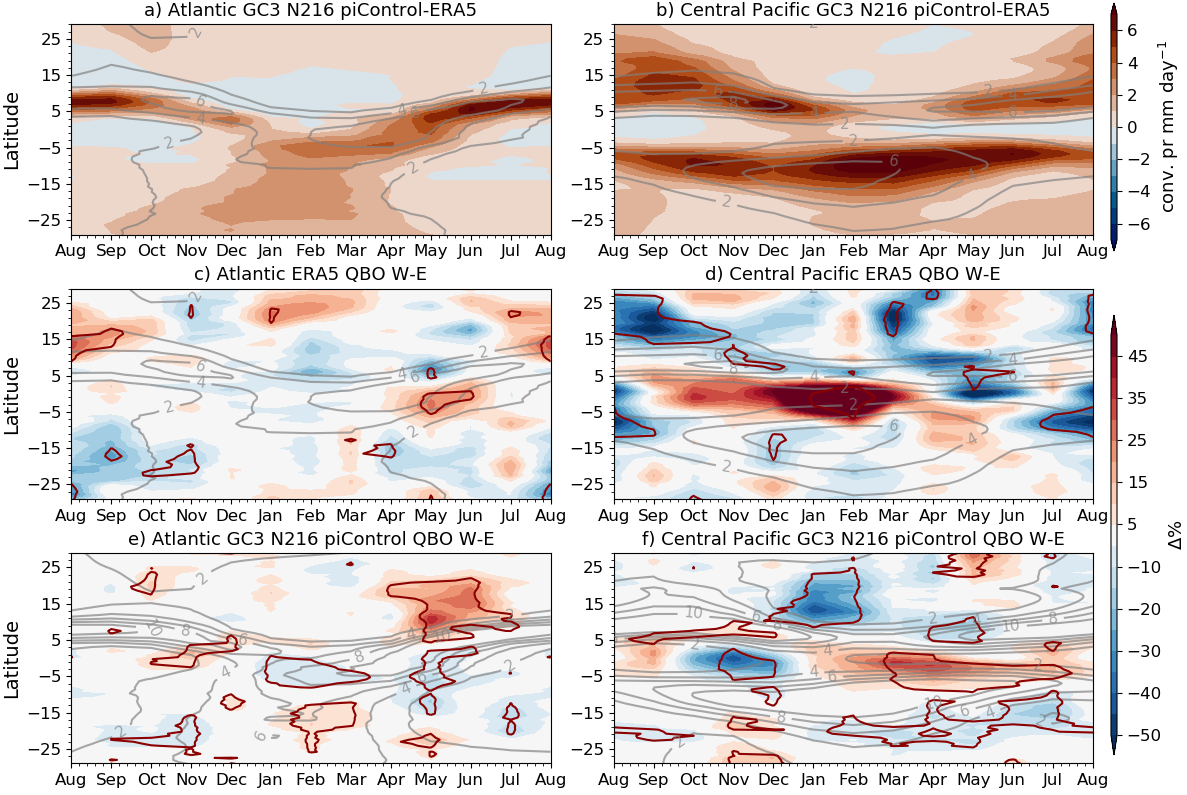
\includegraphics[width=\linewidth]{figures/itcz_conv_prqbow.png}
\caption[Central Pacific ITCZ convective precipitation differences on QBO phase.]{ (a, b) Zonal mean biases in convective precipitation in GC3 N216-pi compared to ERA5 in the (a) Atlantic [60$^\circ$W-20$^\circ$W] and (b) Central Pacific [180$^\circ$W-140$^\circ$W] sectors. (c-f) Monthly and zonal mean QBO W-E percent (\%) differences in convective precipitation  where the absolute difference is weighted by the climatological value at each latitude and month. The line-contour (red) depict differences that are statistically significant to the 95\% level according to a bootstrapping test and the grey lines show the climatological values.}
\label{fig:itczqbowcp}
\end{figure}

This section investigates how the ITCZ, monsoons and the Walker circulation are influenced by the QBO in the model compared to the observations. %The last section found that there are significant precipitation signals that are independent from ENSO, which may be explained by tropical dynamical features.
Climate model biases in the representation of the migration and dynamics of the ITCZ, or in the mean-state of the Walker circulation, may modify any physical effects of the QBO over convection. 
%In GC3 N216-pi, biases in the position and strength of the Pacific and Atlantic ITCZs are smaller than in the lower resolution configurations of the UM model \citep{garciafranco2020} and this configuration has been top ranked in several assessments of tropical precipitation amongst CMIP6 models \citep{abdelmoaty2021biases,richter2020overview}.
For example, ITCZ biases in position or strength (Fig. \ref{fig:itczqbowcp}a-b) are  noteworthy in the model, and are mainly characterized by a southward shift of the simulated Atlantic ITCZ in DJF and MAM and a wider extent of the Central Pacific ITCZ compared to ERA5.

The monthly-mean QBO W-E zonal-mean convective precipitation differences in the Pacific and Atlantic ITCZ regions (Figure \ref{fig:itczqbowcp}) show that the ITCZ impacts are seasonally dependent.
While there are no clear differences in the Atlantic sector for ERA5 in any month, in GC3 N216-pi there is a significant northward shift of the ITCZ from April to June, which is likely associated with the warm SST anomalies found in this season in the northern tropical Atlantic (Fig. \ref{fig:sstclim}). 

\begin{figure}[t!]
\centering
 %\noindent
 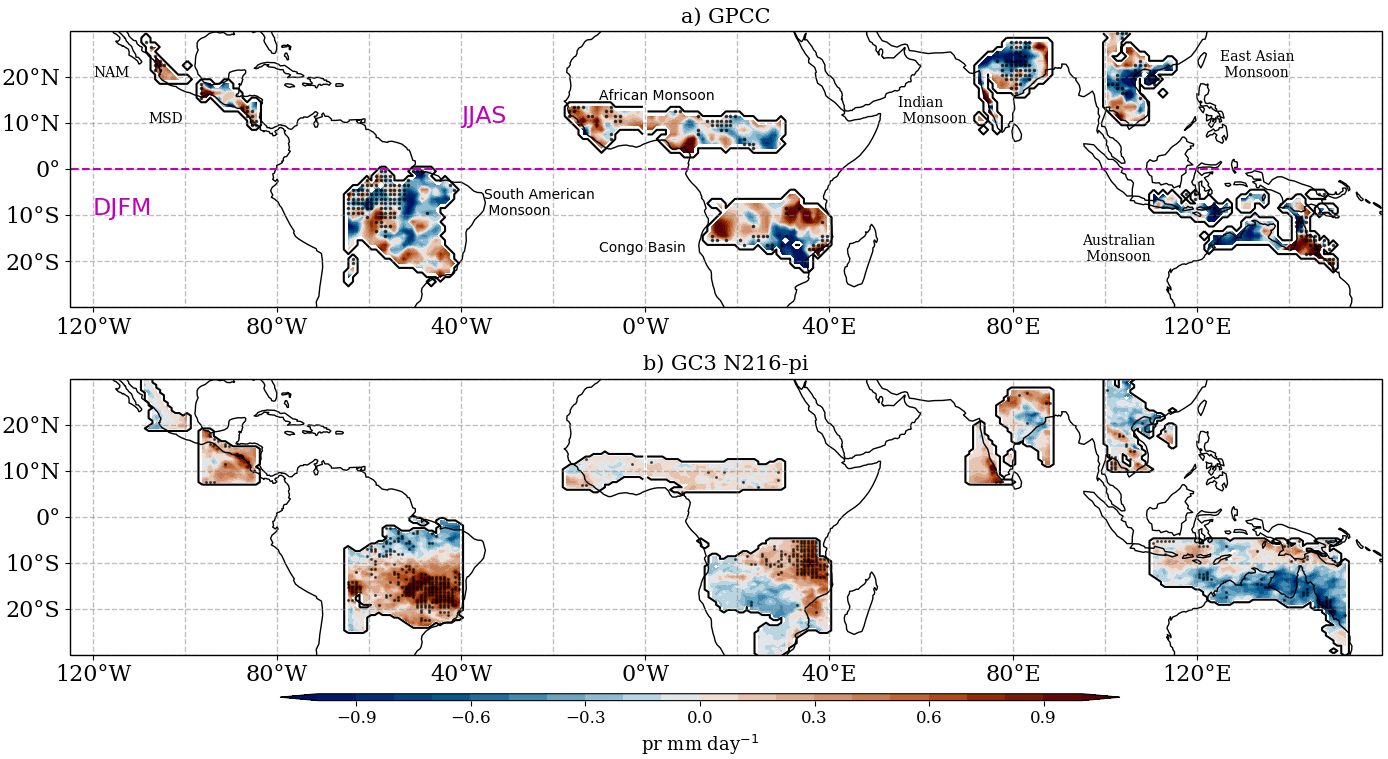
\includegraphics[width=\linewidth]{figures/monsoon_gpcc_qbow.png}
\caption[Global monsoon impacts of the QBO.]{ Convective precipitation differences in monsoon regions between QBO W-E  phases for a) ERA5 and b) GC3 N216-pi. For monsoon regions in the Northern hemisphere, differences are shown for the JJAS period, whereas for Southern Hemisphere monsoons, results are shown for DJFM.  Red dots indicate differences that are statistically significant to the 95\% level according to the bootstrapping test.}
\label{fig:mons_map}
\end{figure}

 The differences in the Pacific sector confirm previous model and observational results \citep{gray2018,serva2021} that the Pacific ITCZ becomes stronger during QBOW compared to QBOE (Fig. \ref{fig:itczqbowcp}d, f). In observations, the strongest differences are found during DJF, characterized by increased precipitation over the core ITCZ regions. In GC3 N216-pi, a stronger ITCZ is observed slightly south of the climatological position from February to July, maximized in the MAM season. Very similar results for the Atlantic and Pacific sectors were observed for the other two simulations (not shown). The result also holds for ENSO Neutral periods (not shown) which rules out the possibility that the Atlantic ITCZ results are due to ENSO teleconnections to the tropical north Atlantic. 


In spite of existing observational evidence \citep{collimore2003,liess2012,gray2018} that suggests a link between the QBO and monsoon regions, the results in the previous sections (Fig. \ref{fig:qboclim}) show little-to-no effect of the QBO on precipitation over land in the simulations. 
The precipitation response over land is examined more closely by analysing regions that fit the concept of the global monsoon. For this purpose, a monsoon region is defined as a region in which over 55\% of the total annual rainfall is observed or simulated in the respective summer season and the summer-winter rainfall rate difference is higher than  2 mm day$^{-1}$ \citep{wang2008,wang2017,wang2021monsoons}. 

After defining these regions, the QBO W-E differences are computed for JJAS and DJFM for Northern and Southern Hemisphere monsoons, respectively. 
Figure \ref{fig:mons_map} shows that there is no coherent response to the QBO phase in  GPCC in any monsoon region. However, in GC3 N216-pi there are significant differences for Southern Hemisphere monsoons. In the South American monsoon region, the QBO W-E differences indicate a significantly wetter region in South America, where the South Atlantic Convergence Zone is located \citep{carvalho2004,jorgetti2014}. Similarly, a drier Australian monsoon and wetter conditions for East Africa are observed during QBOW compared to QBOE.

For Northern Hemisphere monsoons there are no robust or significant differences (Fig. \ref{fig:mons_map}b). However, when only Neutral ENSO months are considered, all three simulations suggest a wetter Central American monsoon (not shown) in QBOW compared to QBOE. 
The different responses observed for the three simulations suggest that the representation of the dynamical features of each monsoon by each model configuration is important for any response to the QBO. Furthermore, the relatively smaller signals seen over land compared to over the oceans suggests that SST feedbacks are important for the QBO response in the model, so that reduced impacts are seen in regions of land convection. 
%These Atlantic SST-ITCZ changes could also explain the response observed South America in Fig. \ref{fig:qbodjf}c-d \citep{yoon2010atlantic}.
 % in agreement with the results of the previous section.

\begin{figure}[t!]
\centering
 \noindent
 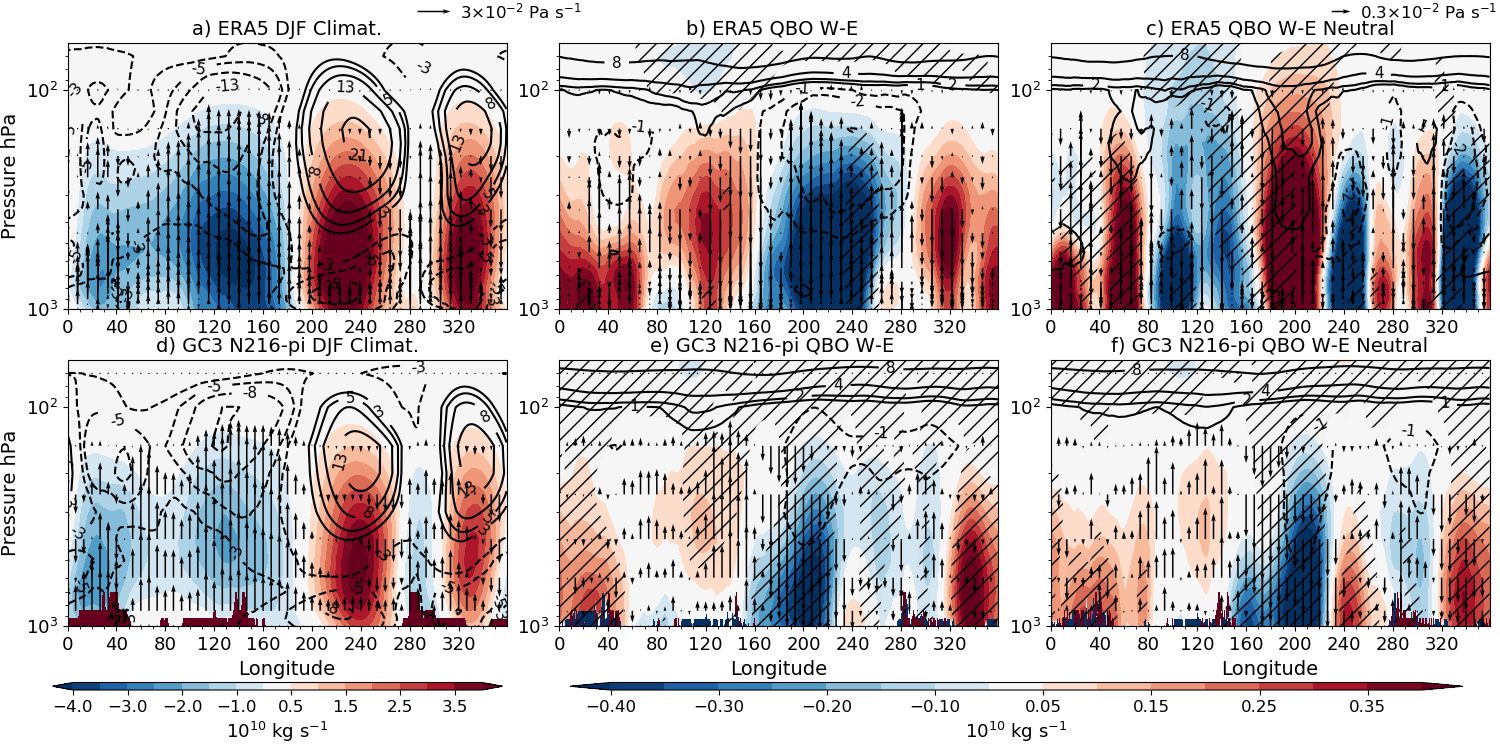
\includegraphics[width=\linewidth]{figures/cmip_era5_streamdjf.png}
\caption[Walker circulation anomalies in DJF]{(a, d) Climatological mean-state of the Walker circulation, depicted through the zonal streamfunction ($\psi$) in shading, the zonal wind (contours), and vertical velocity ($\omega$ [Pa s$^{-1}$], vectors) during the DJF season in a) ERA5 and (b) N216-pi. (b, c, e, f) show W-E composite differences, during DJF, for the same variables only that hatching represents statistical significance to the 95\% confidence level for differences in the streamfunction, and only statistically significant differences in the zonal wind and $\omega$ are shown. (g-h) are as in (d-f) but considering Neutral ENSO periods only. Example vector sizes for $\omega$ are given in the top right corners of a and c.  }
\label{fig:walker_djfm}
\end{figure}

A number of studies have suggested a link between the QBO and the Walker circulation to explain the zonally asymmetric nature of the QBO anomalies in convective precipitation \citep[e.g.][]{collimore2003,liess2012}. To evaluate this hypothesis, the zonal streamfunction is used to measure the Walker circulation \citep{yu2010,bayr2014} and is defined as:

\begin{equation}
\psi=2\pi \frac{a}{g} \int_0^p u_D dp,
\end{equation}

\noindent where $\psi$ is the zonal streamfunction, $u_D$ is the divergence part of the zonal wind, $a$ is the Earth's radius, $p$ is the pressure coordinate and $g$ the gravitational constant.
The streamfunction is calculated by first averaging over the equatorial band of 10$^\circ$S-10$^\circ$N and integrating to the top level of each dataset.

QBOW minus QBOE composite differences in DJF show that the streamfunction in the eastern Pacific [220-260$^\circ$E] is significantly weaker during QBOE than during QBOW in ERA5 and GC3 N216-pi (Fig. \ref{fig:walker_djfm}). These streamfunction differences are significant even low in the troposphere in the model. The zonal wind at upper-levels (300-100 hPa) is also weaker in QBOW compared to QBOE at 200$^\circ$E in both model and reanalysis. In GC3 N216-pi, the negative $\psi$ difference is accompanied by descending motion anomalies in the 170-220$^\circ$E region, whereas anomalous ascent is observed in the Maritime continent and Indian Ocean. The differences in the other simulations agree with the results of GC3 N216-pi (not shown).

\begin{figure}[t!]
\centering
 \noindent
 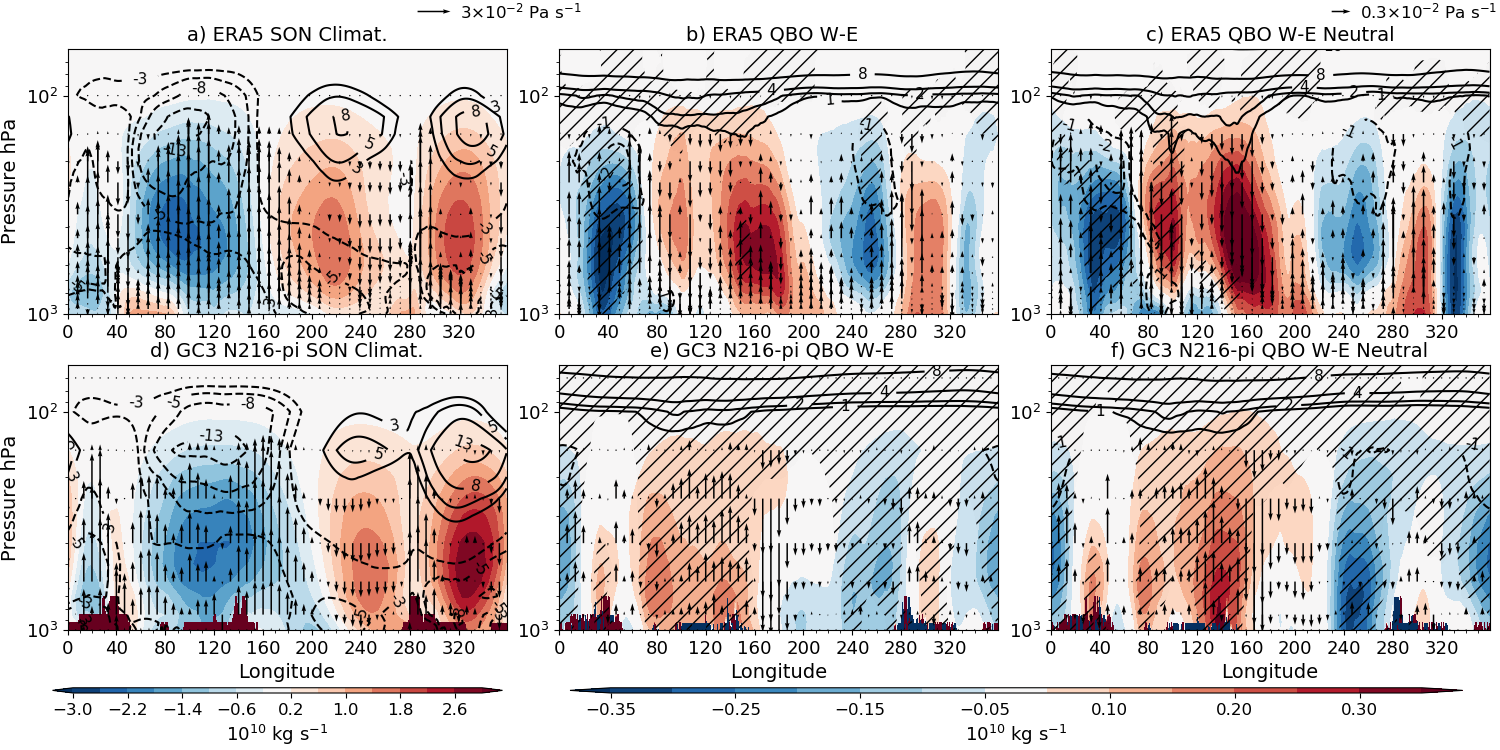
\includegraphics[width=\linewidth]{figures/cmip_era5_streamson.png}
\caption[Walker circulation anomalies in SON]{As in Figure \ref{fig:walker_djfm} but for the SON season. }
\label{fig:walker_son}
\end{figure}

In boreal fall (Fig. \ref{fig:walker_son}), the differences are also significant and are linked to the relationships found between the IOD and the QBO. 
Specifically, significant positive differences in the streamfunction are found 
in the eastern Indian Ocean and maritime continent and negative differences in the eastern Pacific. 
In GC3 N216-pi, vertical velocity anomalies indicate stronger ascent in the western Indian Ocean and in the Maritime continent whereas descending anomalies are found in the eastern Indian Ocean. These results agree with positive IOD indices found in QBOW and a mean negative index during QBOE.



The rightmost panels in  Figures \ref{fig:walker_djfm} and \ref{fig:walker_son}, in which only Neutral ENSO months are considered, suggest that this relationship between the QBO and the Walker circulation occurs regardless of ENSO events for GC3 N216-pi. However in ERA5, removing ENSO events changes the sign of the response, likely due to the small sample size in the observational record when only neutral months are considered. 
These results highlight links between the large-scale overturning circulation and local responses which may explain the zonally asymmetric results found in previous studies and in early sections of this chapter.



\section{The nudging experiments}\label{sq:nudging}

\begin{figure}[t!]
\centering
 %\noindent
 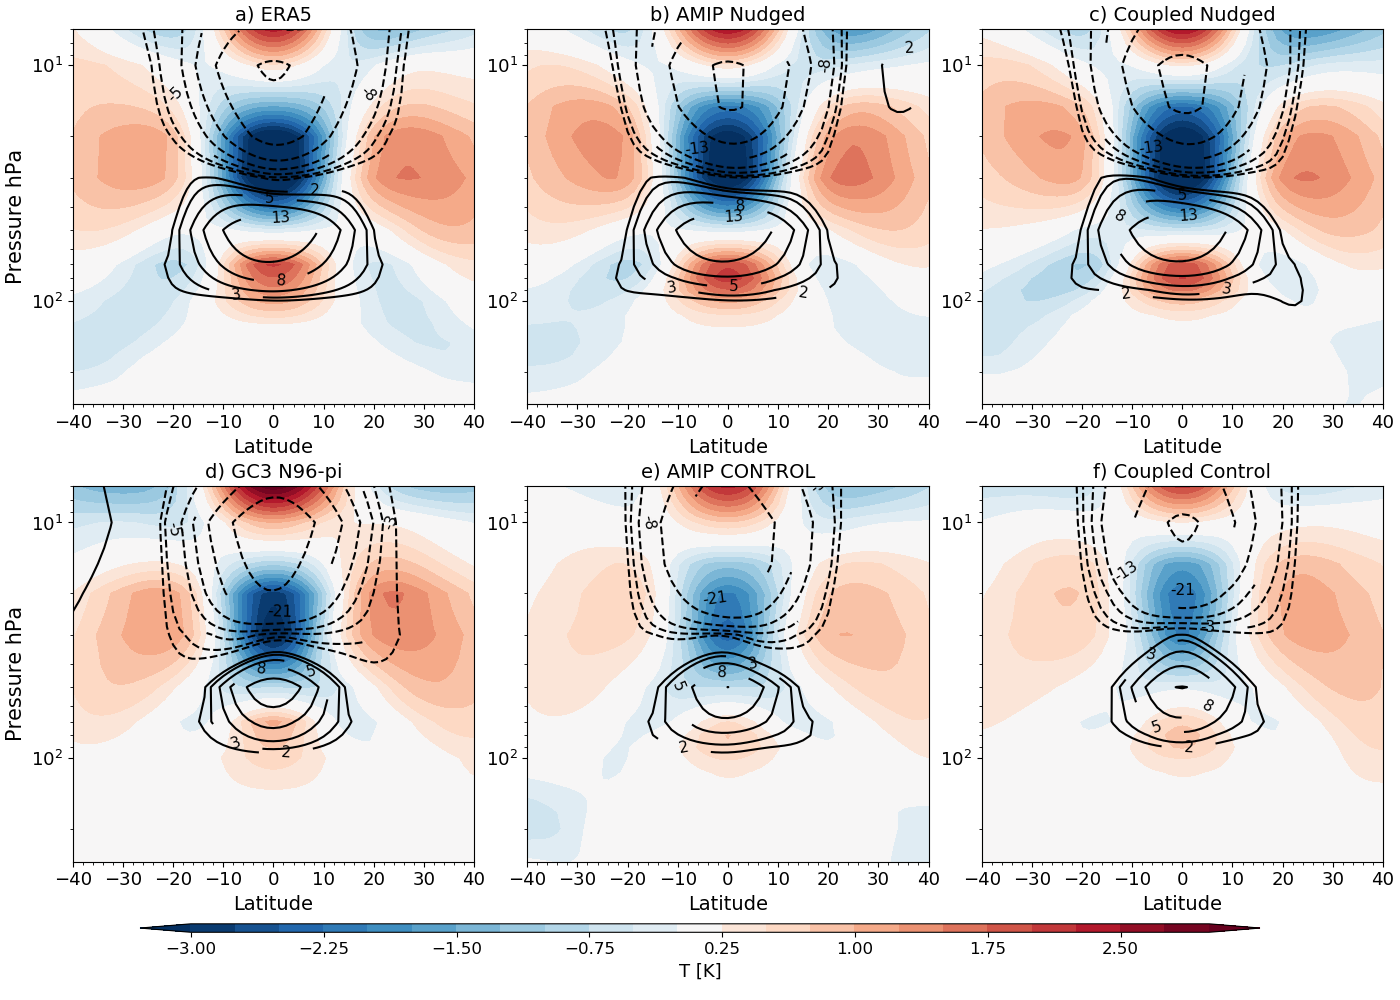
\includegraphics[width=\linewidth]{figures/zonal_thesis.png}
\caption[Zonal-mean zonal wind QBO difference]{Latitude-height plot of the annual and zonal-mean temperature (shading) zonal wind (contours in m s$^{-1}$ differences (QBO W-E) in (a) ERA5, the ensemble-mean nudged simulations in (b) AMIP and (c) coupled configurations and (d) GC3 N96-pi from CMIP6, the control simulations with no nugding for (e) AMIP and (f) coupled configurations. The black line denotes the tropopause height obtained from the model data in (b, d) and for ERA5 the tropopause height was found through the gradient threshold method. For the nudged experiments, the ensemble-mean is shown. The nudging region is illustrated in c), where the red box indicates where the full nudging is applied and the green box illustrates the tapered region. }
\label{fig:zonal_u}
\end{figure}

This section investigates results from a series of nudging experiments in which the equatorial zonal winds in various configurations of the HadGEM model were relaxed towards ERA5 (between 10$^\circ$S-10$^\circ$N, full nudging was applied from 10 hPa to 70 hPa, tapering to zero by 90 hPa; see section \ref{nudg_setup} for full details). Nudging the QBO winds towards observations means that feedback from the modelled tropospheric processes onto the QBO is eliminated. Examination of the QBO signal at the surface then allows an investigation of the QBO influence on the modelled tropospheric or surface fields. Nudging the fields also serves to correct a bias in the equatorial lower stratosphere where the model underestimates the amplitude of the QBO. The model has been run in both AMIP and coupled ocean configurations to explore the role of the ocean, since results from previous sections show a strong dependence on ENSO phase. Additional AMIP sensitivity experiments are also performed, to further test the importance of consistency between SSTs and the QBO phase. Parallel Control simulations were performed for each experiment, identical in all respects apart from the nudging (see Table \ref{tab:nudg_exps} for details of the experiments, including length of the simulations and numbers of ensembles performed).  The idealised experiments are then used to investigate the static stability hypothesis for the tropical route of QBO teleconnections with the surface.  

Before proceeding to analyse the surface response, we first show the QBO impact in UTLS  
temperatures and zonal winds (Figure \ref{fig:zonal_u}) from the nudged experiments compared to ERA5 and the 500-yr CMIP6 GC3 N96-pi simulation, as well as the Control experiments in which the QBO is free-running instead of being nudged.  The QBO W-E differences in the nudged experiments closely resemble the ERA5 field, confirming that the nudging has been successful. Both temperature and wind differences are larger in the nudged experiments compared to the non-nudged experiments at all heights over the equator, especially in the region just above the tropopause between $~$70-100 hPa, confirming also that the weak QBO amplitude bias in the lower-stratosphere has  
been removed by the nudging.  

\subsection{Atmosphere-only experiments}


\begin{figure}[t!]
\centering
 %\noindent
 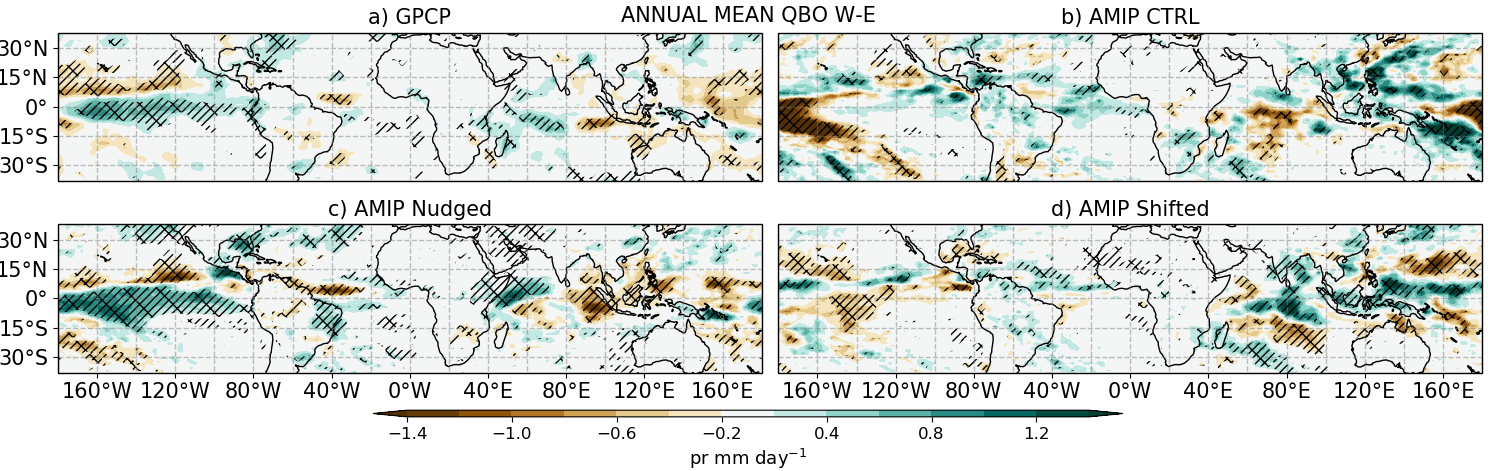
\includegraphics[width=\linewidth]{figures/pr_amip_climqbowqboe.png}
\caption[Annual mean precipitation response in atmosphere-only experiments]{Annual-mean precipitation response (QBO W-E) in (a) GPCP, and atmosphere-only experiments: (b) AMIP CTRL, (c) AMIP Nudged and (d) AMIP Shifted.  }
\label{fig:amip_clim}
\end{figure}

This section describes the results of the atmosphere-only experiments: AMIP Nudged, 
AMIP Control and AMIP Shifted (in which the imposed SSTs have been shifted by a year so there is an out-of-phase relaxation of the winds with respect to the SSTs). The annual-mean difference of precipitation between QBOW and E phases from the three experiments are compared with GPCP differences in Fig. \ref{fig:amip_clim}. The AMIP Nudged ensemble-mean matches closely the results of GPCP, characterised by an El Niño pattern in the Pacific Ocean, a weaker Atlantic ITCZ and a zonal gradient of precipitation in the Indian Ocean (the IOD) during QBOW compared to QBOE. In contrast, the AMIP Control and the AMIP Shifted experiments fail to reproduce the observations. A similar result is found for seasonal-mean composite differences (not shown). 

It is interesting to compare the results of the AMIP Control experiment (Figure \ref{fig:amip_clim}b) with the corresponding CMIP6 coupled GC3 N96-pi results (Figure \ref{fig:qboclim}b) which reproduced the observations reasonably well, albeit with reduced amplitude. Although we note that the CMIP6 model set-up is not entirely identical to these experiments since the model configuration is slightly different, the major difference between them is the lack of a coupled ocean in AMIP Control. The failure of AMIP Control to simulate the observations therefore suggests an important role for the oceans in the surface response to the QBO. 
Moreover, the Shifted and Nudged experiments show markedly different responses, suggesting that the alignment between stratospheric winds and SSTs is key to reasonable simulate the response in AMIP Nudged. 

\begin{figure}[t!]
\centering
 %\noindent
 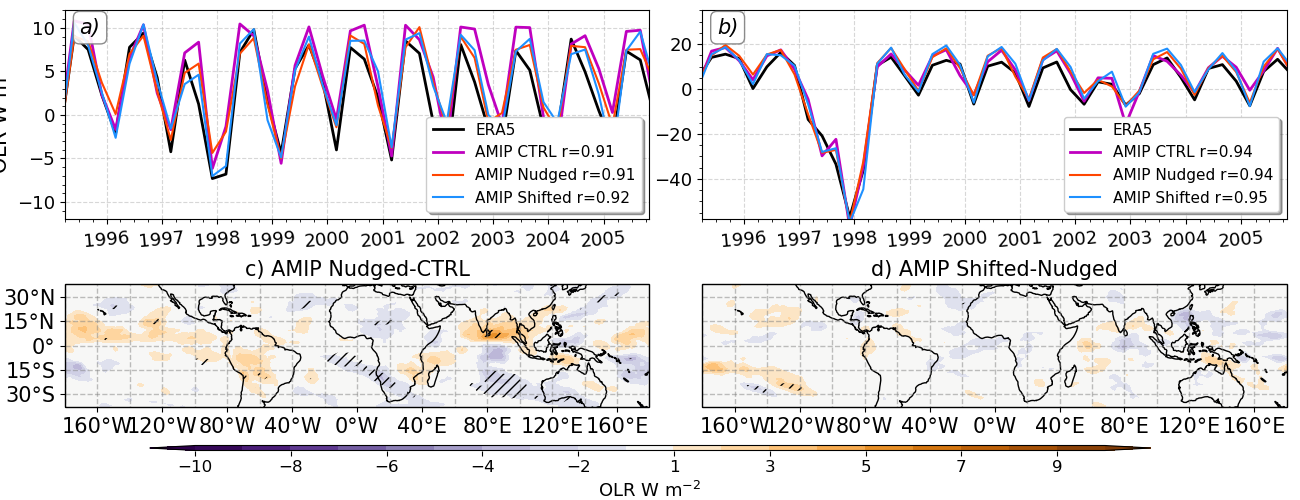
\includegraphics[width=\linewidth]{figures/olr_amip.png}
\caption[OLR time-series and spatial pattern differences in AMIP experiments]{(a, b) Time-series of (a) zonal-mean equatorial [5$^\circ$S-5$^\circ$N], and (b) area-averaged EN3.4 OLR in ERA5 and the three amip experiments. For each AMIP experiment the Pearson correlation coefficient between the experiment time-series and ERA5 is shown in the legend. (c) Differences in mean OLR between AMIP Nudged and Control and (d) between AMIP Shifted and Nudged. Significant (95\% confidence level) differences according to a Mann-Whitney U test in (c, d) are highlighted with hatching. }
\label{fig:olr_amip}
\end{figure}

%As a check of whether the nudging has modified the mean or variability of the troposphere, OLR in the tropics is examined and compared in the AMIP experiments.
The time-series of equatorially averaged OLR, shown in Fig. \ref{fig:olr_amip}a, suggests that the nudging has not had a direct influence on the underlying tropospheric processes, especially on the characteristics of tropical deep convection. The OLR is almost indistinguishable between the three AMIP experiments and agree well with ERA5. Similar results are found for OLR averaged in the EN3.4 region (Fig. \ref{fig:olr_amip}b). The correlation coefficients of the time-series also indicate no difference between the experiments. Examination of the spatial OLR distributions also shows no robust differences in the Pacific between the Control and AMIP Nudged (Fig \ref{fig:olr_amip}c) nor between the AMIP nudged and AMIP Shifted experiments (Fig. \ref{fig:olr_amip}d), confirming that the nudging has had no effect on the mean state or variability of OLR in the AMIP experiments. 

\begin{figure}[t!]
\centering
 %\noindent
 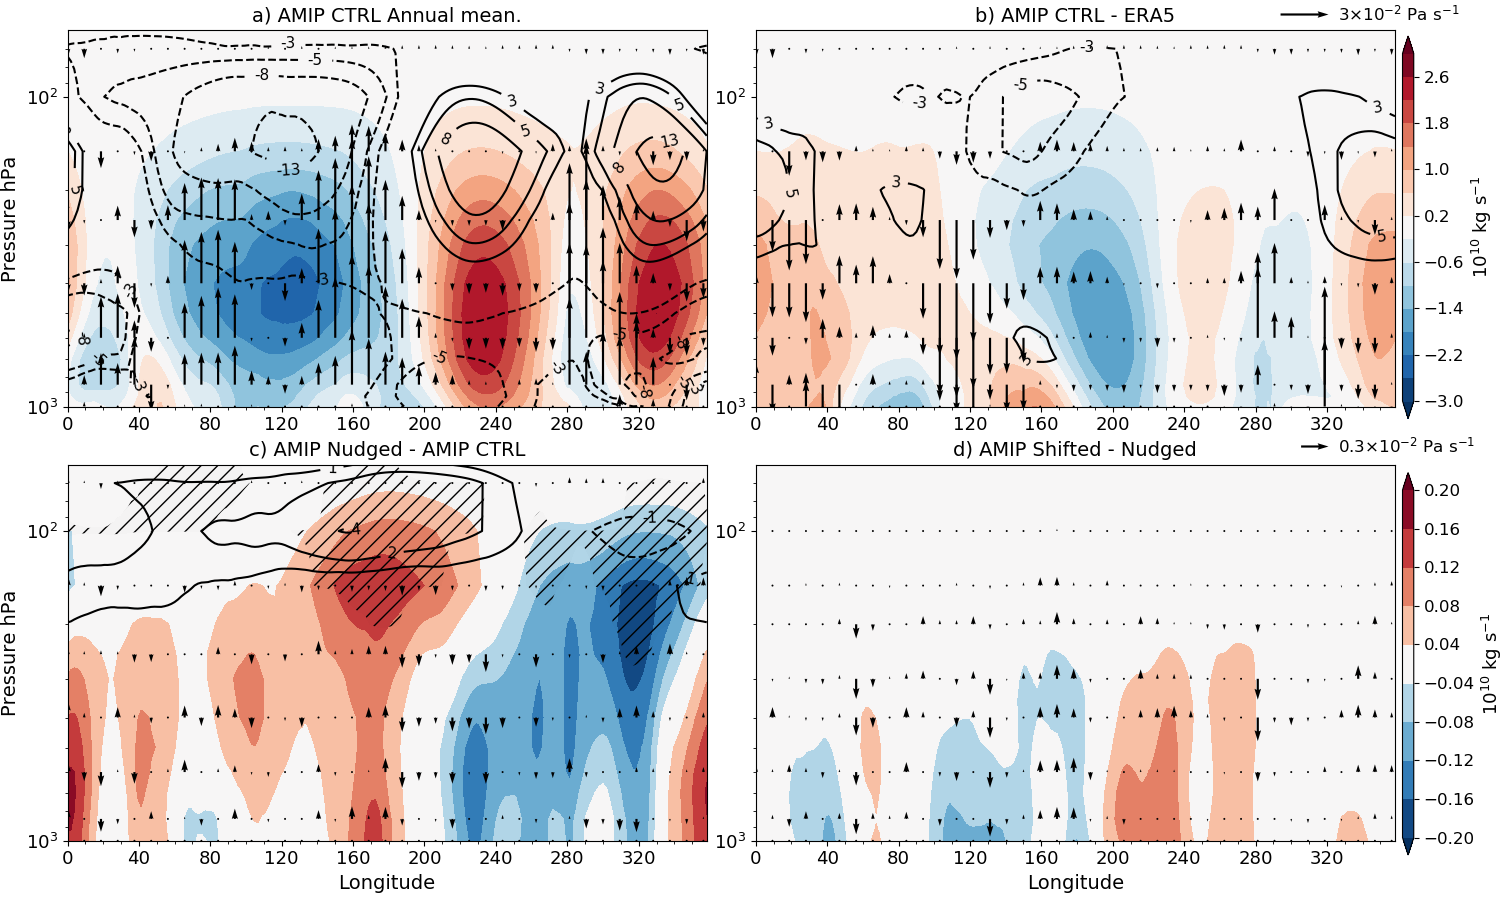
\includegraphics[width=\linewidth]{figures/suite_streamwalkerclim.png}
\caption[Walker in atmosphere-only experiments]{Zonal mass streamfunction ($\psi$ in shading), zonal mean zonal wind (contours) and vertical velocity (vectors) averaged over the band 10$^\circ$S-10$^\circ$N. Climatological mean in the (a) AMIP Control experiment and (b) ERA5. (c-d) show biases in the (c) Control and (d) Nudged experiments with respect to ERA5 whereas (e-f) show differences between experiments, (e) AMIP Nudged-Control and (d) AMIP Shifted-Nudged. Note that the colorbar and scale of the vectors changes are different between (a-d) and (e-f). In (e-f), significant differences (95\% confidence level according to a Mann-Whitney two-sided test) in the streamfunction are highlighted with hatching. }
\label{fig:walkeramip}
\end{figure}


Diagnostics of the overturning circulation in the AMIP Control and ERA5 are compared in Figure \ref{fig:walkeramip}. The mean state of the Walker circulation is weaker in the AMIP Control simulation and exhibits an easterly bias at upper levels compared to ERA5 (Fig. \ref{fig:walkeramip}c). The Walker circulation biases in the upper troposphere of the control experiments (Fig \ref{fig:walkeramip}c) are improved in the nudged experiments (Fig. \ref{fig:walkeramip}d,e). Even though the relaxation is only applied above 90 hPa, significant differences between control and nudged experiments are observed for the zonal wind and streamfunction at 200 hPa near the dateline, over South America and over the Atlantic Ocean. 

However, no significant differences in the streamfunction or zonal wind in the lower troposphere are observed between the AMIP Shifted and Nudged experiments (Fig \ref{fig:walkeramip}f). The lack of any difference between the two nudged experiments, which differ only in a 1-year shift of the prescribed nudging winds, means that the variability of the imposed winds is not important for the mean state of the Walker circulation. %, and is consistent with the findings of precipitation and OLR.

This section has shown that nudging the QBO towards ERA5 zonal winds has corrected the bias in lower stratospheric winds (Figure \ref{fig:zonal_u}) which has also improved the upper-level tropical overturning circulation (Figure \ref{fig:walkeramip}). However, the major result is that the precipitation response depends crucially on the SSTs, since the QBO signal in precipitation is entirely different betweeen the AMIP Nudged and Shifted experiments. The results thus demonstrate that the QBO signal in precipitation is primarily due to the QBO signal in the underlying SSTs.
 The direct influence of the improved QBO winds and temperature variability in the UTLS for tropical deep convection seems to be of secondary importance relative to the SST forcing. However, because the SSTs are imposed in the AMIP model configuration, the source of the QBO signal in SSTs and the nature of any feedback mechanism between the QBO and the SSTs cannot be addressed. For this reason, next we present the results from the simulations using the coupled model configuration.  


\subsection{Coupled experiments}

\begin{figure}[t!]
\centering
 %\noindent
 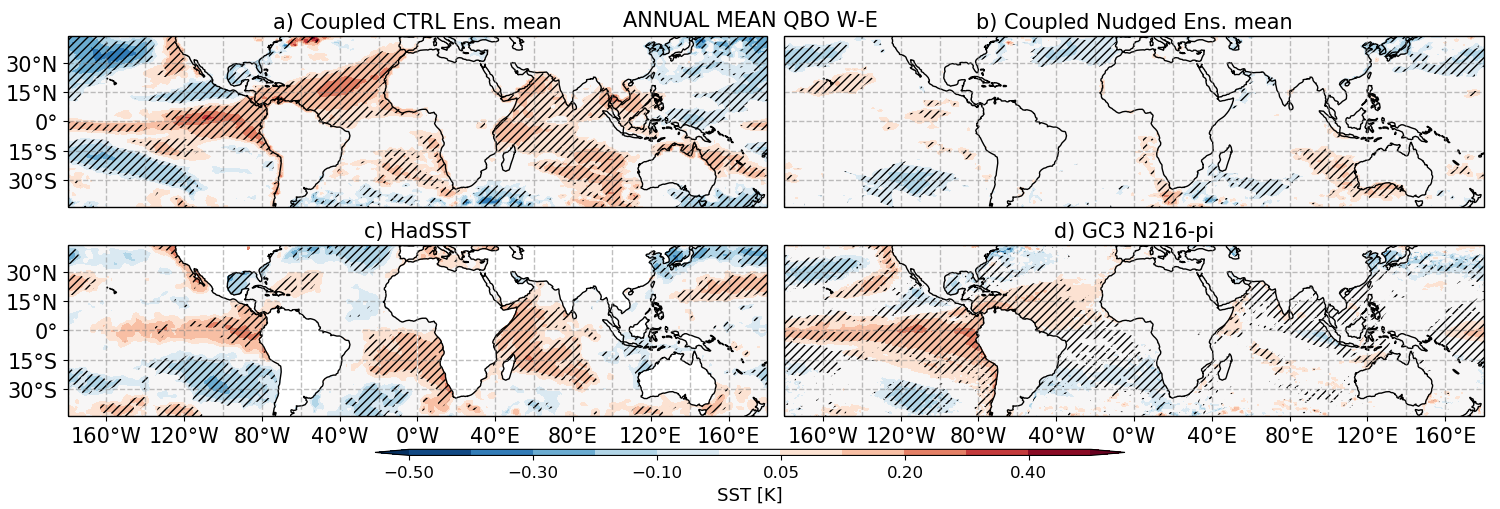
\includegraphics[width=\linewidth]{figures/sstseasonal_climqbowqboe.png}
\caption[Annual mean SST response to the QBO in coupled nudged experiments]{ Annual mean SST [K] QBO W-E differences in (a) Coupled Control and (b) Coupled Nudged ensemble mean, and the (c) HadSST dataset and (d) GC3 N216-pi datasets. Hatching denotes significance to the 95\% confidence level according to a bootstrapping with replacement test.}
\label{fig:sst_clim_coupled}
\end{figure}

This section describes the results from the two experiments that were performed using the coupled ocean-atmosphere configuration of the model. Two control simulations (Coupled Control) were performed, each of 35-years, initialised with slightly different initial conditions (see section \ref{nudg_setup}). A further six 35-year ensemble experiments (Coupled Nudged) were performed that were identical to the Coupled Control simulations except that the QBO nudging was applied in the same region of the equatorial stratosphere as in the AMIP experiments described above. 


The annual mean QBO W-E difference in tropical SSTs in the ensemble-mean of the coupled control experiments (Fig \ref{fig:sst_clim_coupled}a) compares well with the corresponding fields from HadSST and GC3 N216-pi. As discussed earlier (in section \ref{qbo7_enso}) the  QBO W-E responses are characterized by warm signals in the East  
Pacific, and in the northern tropical Atlantic and Indian Oceans.  
The ensemble-mean of the QBO-nudged experiment, however, shows a very weak or null response (Fig. \ref{fig:sst_clim_coupled}b) in all of these regions. 

To examine this further, Fig \ref{fig:sst_ens} shows the individual QBO W-E differences from the 6 ensemble members. The weak response in the ensemble-mean is clearly the result of very 
different responses from each ensemble member, which cancel out to a large extent. 
The individual seasonal-mean diagnostics show a similar behaviour (not shown). The results suggest that when the nudging is applied to the model a key feedback process between the QBO and SSTs has been suppressed and internal variability dominates over the effect of the imposed winds, if any. 

\begin{figure}[t!]
\centering
 %\noindent
 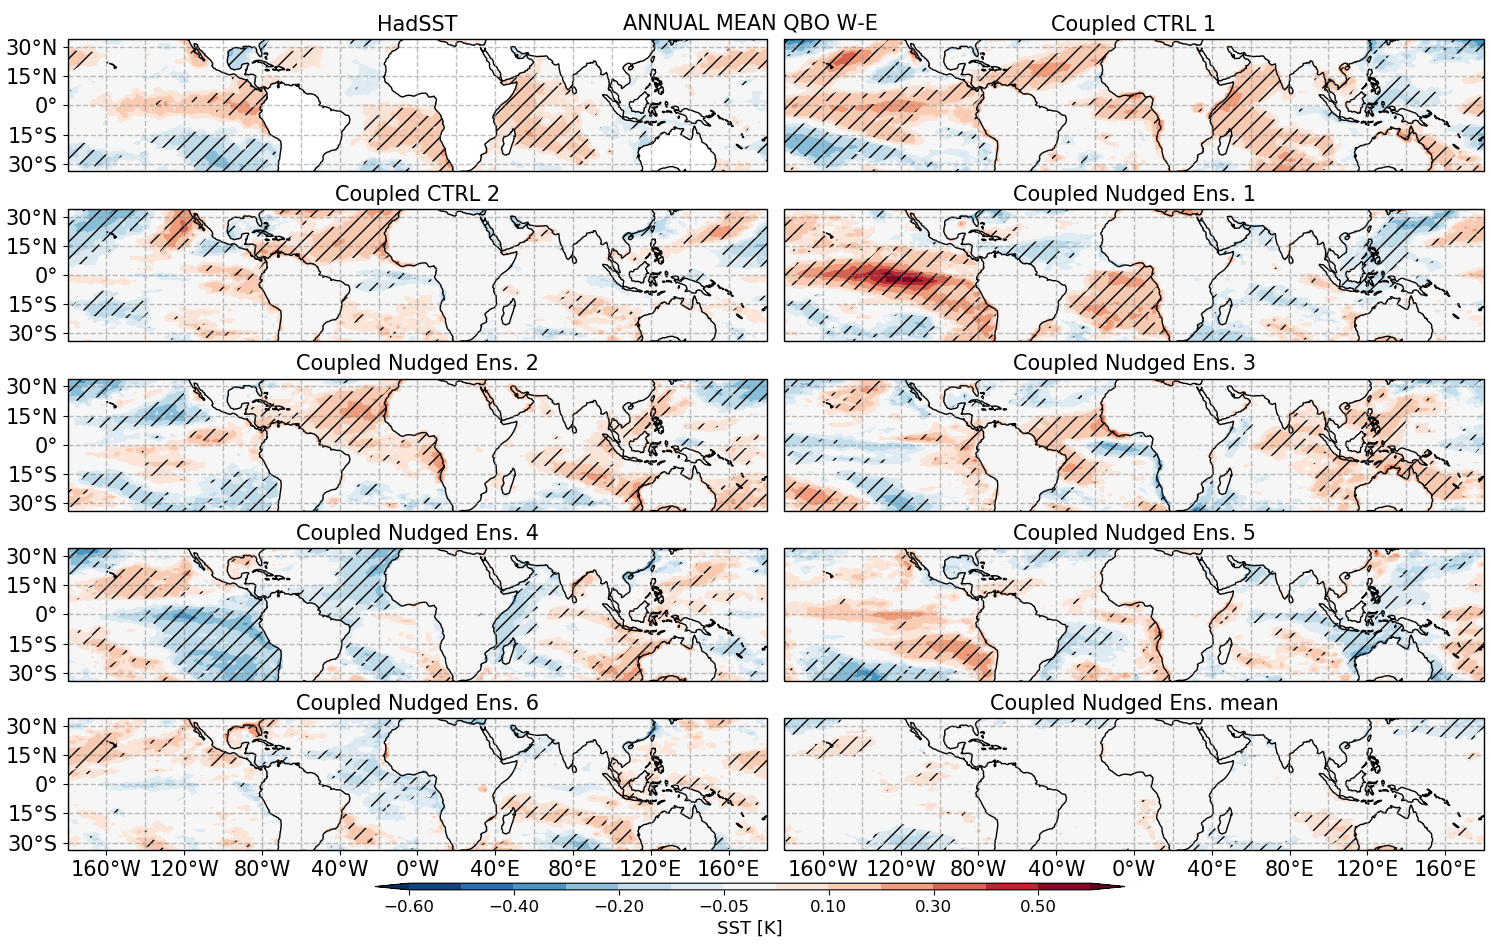
\includegraphics[width=\linewidth]{figures/sst_check_climqbowqboe.png}
\caption[SST response in MAM to the QBO in coupled nudged experiments]{Annual-mean SST differences between QBO phases in the HadSST dataset and the individual ensemble members fromm the Coupled Control and Coupled Nudged simulations.}
\label{fig:sst_ens}
\end{figure}



\begin{figure}[t!]
\centering
 %\noindent
 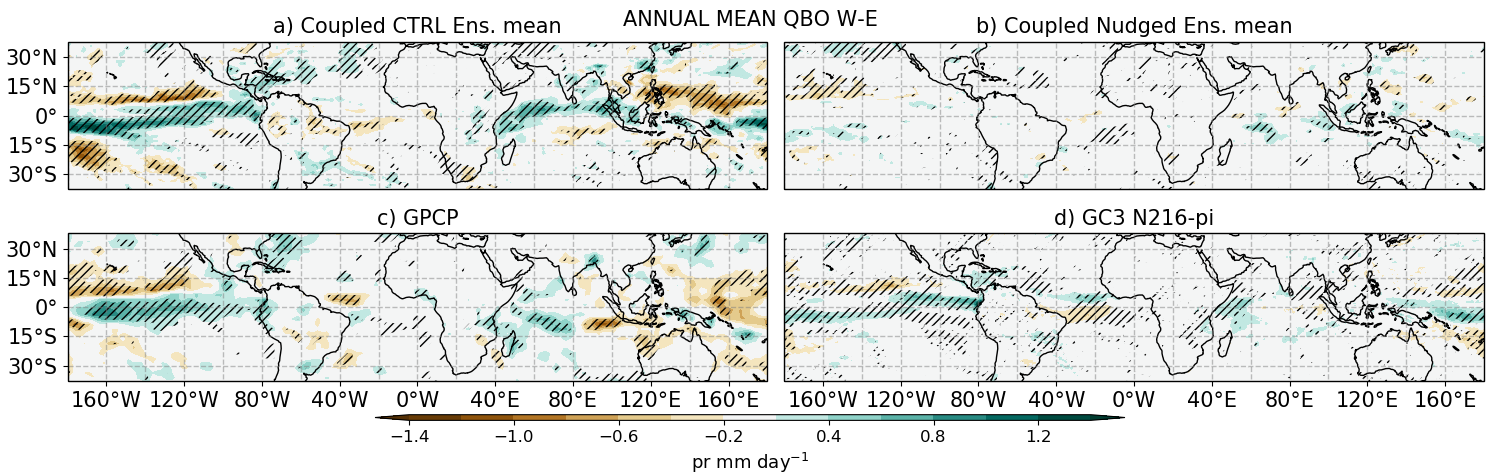
\includegraphics[width=\linewidth]{figures/prseasonal_climqbowqboe.png}
\caption[Annual mean SST response to the QBO in coupled nudged experiments]{ As in Fig, \ref{fig:sst_clim_coupled} but for precipitation [mm day$^{-1}$] using (c) GPCP as the observational dataset.}
\label{fig:pr_clim_coupled}
\end{figure}

The precipitation response is also weaker when the nudging is applied to the coupled 
configuration simulations. The annual mean difference between QBO phases (Fig. \ref{fig:pr_clim_coupled}) in the control experiments show two significant QBO W-E differences: a significant El Niño-like response over the Central and Eastern Pacific Ocean, and a wetter western Indian Ocean. These two precipitation responses are also observed in GPCP and GC3 N216-pi. 

\begin{figure}[t!]
\centering
 %\noindent
 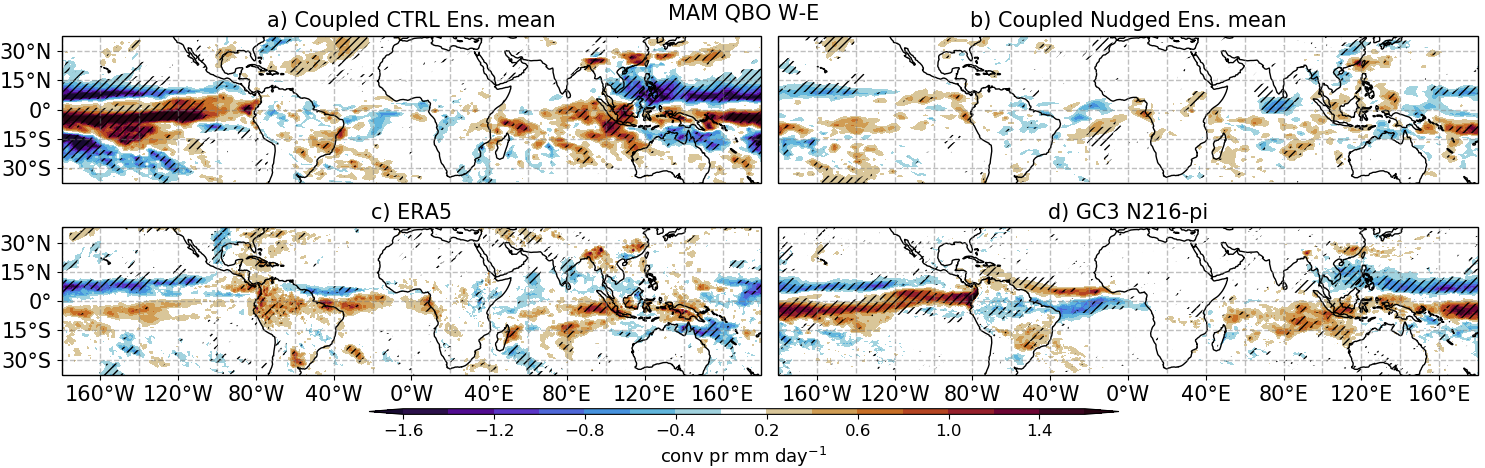
\includegraphics[width=\linewidth]{figures/conv_prseasonal_mamqbowqboe.png}
\caption[SST response in DJF to the QBO in coupled nudged experiments]{ As in Figure \ref{fig:pr_clim_coupled}, but for the MAM season and convective precipitation.}
\label{fig:pr_mam_coupled}
\end{figure}

The ensemble-mean of the nudged experiments, however, shows no robust or region-wide significant differences (Fig. \ref{fig:pr_clim_coupled}b). The weaker response in the ensemble-mean of the nudged experiments is also due to opposing responses found in each ensemble member which cancel out. In specific seasons, robust QBO W-E responses in convective precipitation are observed in the Control experiments, ERA5 and GC3 N216-pi, for example, a meridional dipole in the Pacific Ocean (Fig. \ref{fig:pr_mam_coupled}) and a wetter eastern Indian Ocean during MAM. These results confirm that the control experiments exhibit QBO-related precipitation impacts similar to those found in the CMIP6 experiments and in some instances also similar to the observed impacts. However, these precipitation anomalies disappear in the nudged experiments. 


\begin{figure}[t!]
\centering
 %\noindent
 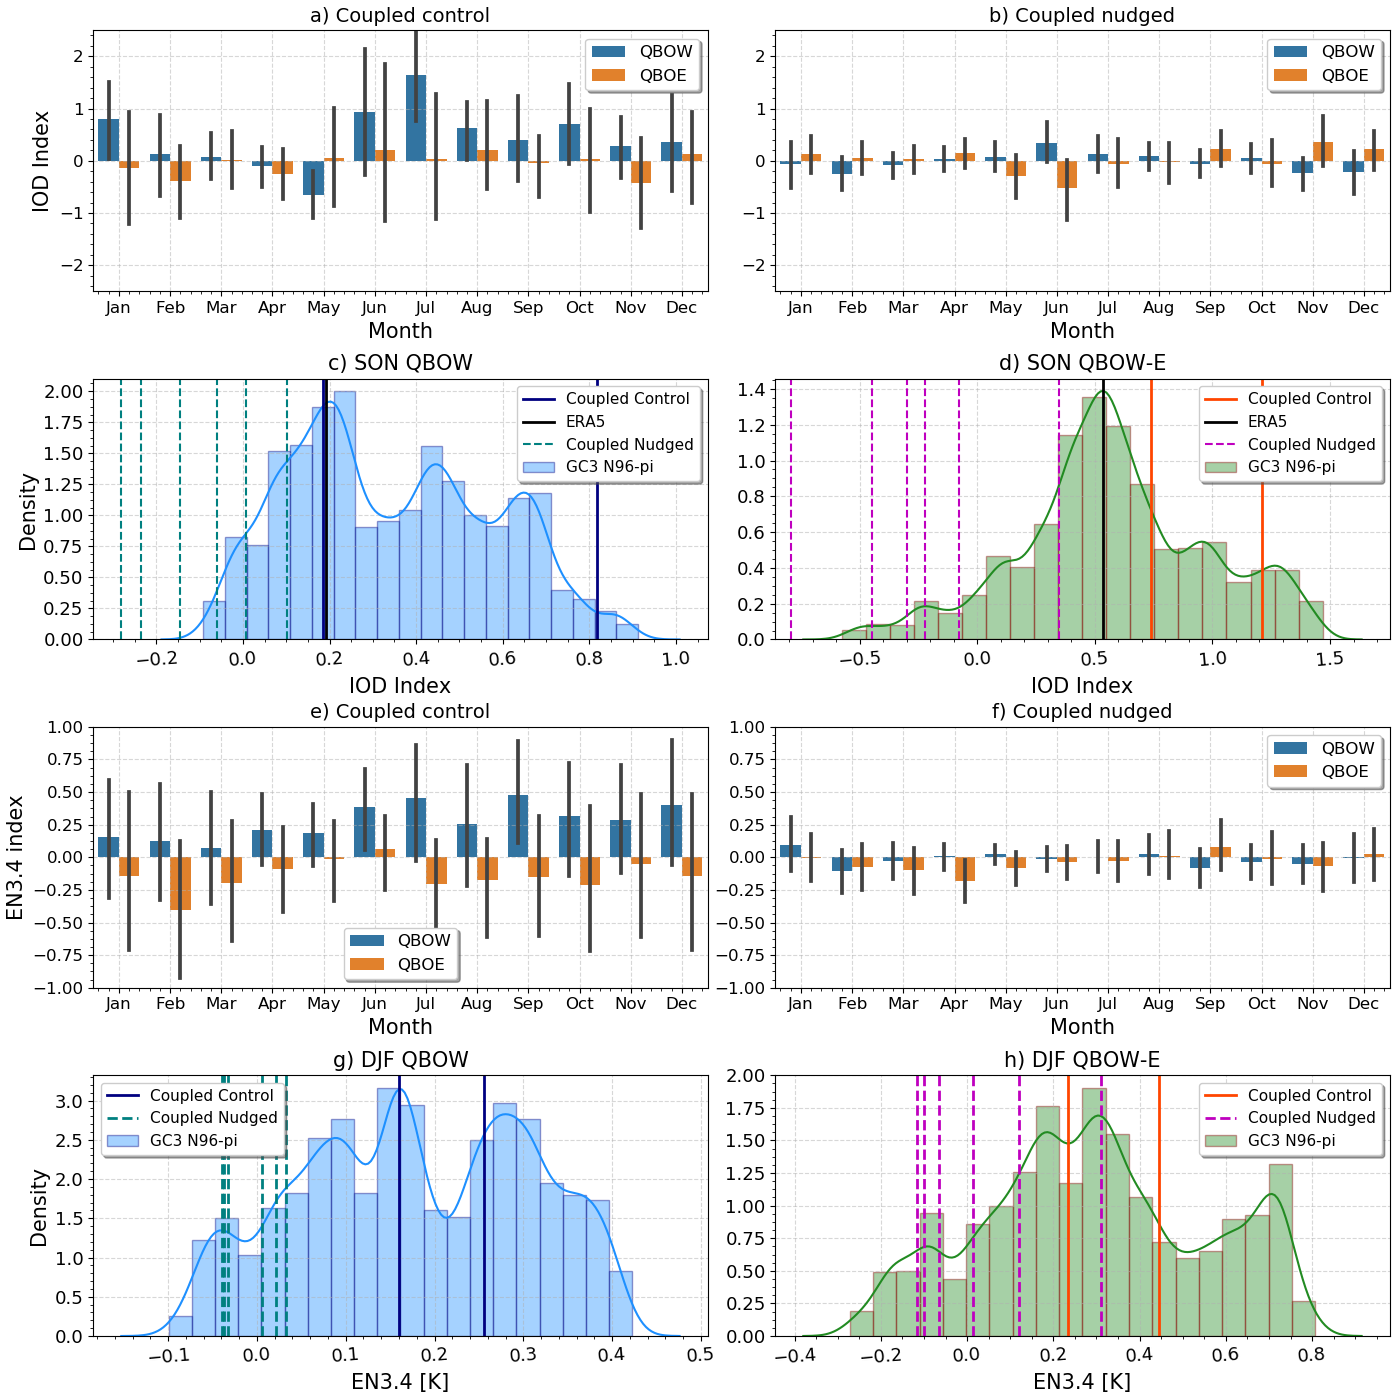
\includegraphics[width=0.97\linewidth]{figures/iod_suites.png}
\caption[IOD and ENSO indices in nudged versus control experiments]{(a, b) Monthly-mean convective precipitation IOD index [mm day$^{-1}$] in coupled (a) control and (b) nudged ensemble-means separated by QBO phase. (c, d) Probability density functions (PDFs) of the IOD convective precipitation index for (c) the mean SON during QBOW months and (d) the SON difference between QBO W-E. The PDF is obtained from the 500 yrs of the GC3 N96-pi by bootstrapping 10,000 times into 35-yr periods and obtaining the averages and differences in each subsample. (e-f) as in (a, b) but for monthly-mean EN3.4 index [K] in the ensemble mean (e) Coupled control and (f) Coupled Nudged simulations separated by QBO phase. (g-h) as in (c-d) but for the EN3.4 index in DJF. }
\label{fig:iod_suites}
\end{figure}

Robust relationships between the QBO phase, and IOD and ENSO indices are also observed in the CMIP6 experiments  (see section \ref{sq:iod_enso}). Figure \ref{fig:iod_suites} shows the mean values of ENSO 
and IOD indices from the nudged and control experiments. The coupled control experiments (Figs. \ref{fig:iod_suites}a, e) show a significant difference for both IOD and ENSO indices identical to the CMIP6 results, i.e., both indices tend to be positive under QBOW and negative under QBOE. For the IOD index, these differences are observed from Jul-to-Jan and for ENSO the differences are found almost year-round but are stronger during boreal fall and winter. However, the nudged ensemble-mean shows no relationships between these indices and the QBO phase. 

To check the robustness of these results, the long CMIP6 pi-control simulations were analysed by computing QBO W-E differences of the indices for 35-yr long randomly selected periods iteratively 10,000 times. The selection of 35-yr periods is to match the length of the observed period in order to investigate how likely is it to find a QBO W-E difference value if the pi-Control simulations were of the same length as observations. This approach leads to a probability density function (PDF) of QBO W-E differences that aims to estimate the impact of internal variability on our ability to extract the QBO signal within the long pi-Control integration and to evaluate how these shorter 35-year coupled experiments fit within those distributions, with and without nudging. 


Figure \ref{fig:iod_suites}d, for instance, shows that the QBO W-E differences in the SON IOD index are predominantly positive in the GC3 N96-pi distribution, and the differences in the two ensembles members of the control experiment are positive as well. However, the Coupled Nudged ensemble members are mostly negative and two of them fall outside the 99\% low end of the PDF.
The EN3.4 index is also more frequently positive under QBOW (Fig. \ref{fig:iod_suites}g) than under QBOE in the CMIP6 and control experiments. There seems to be some indication that the response from the ensemble members of the nudged experiment cancel each other to an ensemble-mean difference of 0. However the PDF of the long CMIP6 piControl does show some density of frequency for non-zero differences, which indicates that periods with no QBO signal are not unlikely in the model. % difference is 

This section shows that in the coupled configuration experiments there are notable
QBO-related impacts that disappear when nudging is applied to the model. In the control 
experiments, impacts over the ITCZs, ENSO and the IOD, to name a few, are robust and similar to results from observations and the longer CMIP6 integrations of the model. However, in the nudged experiments, little-to-no robust responses were observed, as each ensemble member exhibited a different response, leading to a cancellation of the differences in the ensemble-mean. The implications of these results for the stratospheric-tropospheric coupling and QBO teleconnections are discussed in the following section.  

\section{Summary and discussion}

Analyses of observational records of precipitation have long suggested links between the stratospheric QBO and tropical deep convection \citep{collimore2003,liess2012,gray2018}.
However, the short available observational record (<40 years) and the confounding influence of ENSO and its teleconnections limits the robustness of any analysis seeking to explore these links and possible mechanisms of interaction between the QBO and tropical surface climate. The first part of this chapter investigates the tropical signature of the QBO in 500-year-long pre-industrial control CMIP6 experiments, with a focus on the HadGEM3 GC3.1 N216 simulation. 

Composite and regression analyses were used to demonstrate that statistically significant links are simulated by the model between the QBO and several tropical climate features.
Results show robust precipitation responses over the Pacific and Indian Oceans and in some seasons in the tropical north Atlantic. The QBO signal was found to be zonally asymmetric, with the more robust and largest differences found over the oceans, suggesting the possibility of SST feedback processes. The modelled QBO signals agree well with observational analyses and the length of the simulation allows for improved estimation of statistical significance and further exploration of the possible source of these signals.   

The possibility of aliasing of the QBO and ENSO signals and their interaction was extensively explored, using the model simulations. When only ENSO-neutral years are analysed the QBO signal remains essentially unchanged, ruling out the possibility of a straightforward aliasing of ENSO events with the QBO phase selection. The possibility that the apparent QBO signature at the surface is due to an ENSO bias in selection of the QBO phase was also considered. An influence of ENSO on the descent rate and amplitude of the QBO, via modulation of tropical wave generation, has been proposed \citep{schirber2015}. However, while the model was found to successfully simulate the well-known difference in QBO descent rates in which the QBOW phase descends more rapidly than the QBOE phase, there was no evidence for an ENSO influence on the rate of descent or amplitude of either QBO phase.        

This analysis therefore provides evidence for a QBO influence on tropical surface climate that is not simply due to aliasing or a bias in how the QBO index is determined. However, the QBO response patterns strongly suggest that any QBO influence is likely to involve processes such as deep convection and tropical circulation patterns that are also influenced by ENSO. Potential pathways of interaction between the QBO and ENSO signals were therefore explored. While recognising that linear diagnostics are unable to provide specific evidence of cause and effects, they may nevertheless identify candidate mechanisms that are worth exploring more fully.  

 

The frequency of ENSO events in each phase of the QBO was first explored. In observations, El Niño events have been found to occur more frequently in QBOW years and La Niña events are more frequently found in QBOE years \citep{taguchi2010}, suggesting a non-linear interaction of ENSO with the QBO. This dependence was successfully reproduced in the model, providing supporting evidence that the observed QBO-ENSO relationship is not due to observational uncertainty. Similarly, examination of month-by-month ENSO amplitude and interannual variability in the model showed that the interaction between QBO and ENSO is far from linear, since the amplitude dependence on QBO phase was asymmetric. The non-linearity of the QBO-ENSO interaction was confirmed using composites that showed different QBO signal patterns during El Niño years compared with La Niña years. 

In addition to the QBO-ENSO link, the model analysis of total precipitation also highlighted a statistically significant QBO signal in the Indian Ocean, raising the possibility of an interaction with the Indian Ocean Dipole (IOD). In boreal fall the IOD index, which measures the zonal gradient of precipitation in the Indian Ocean, was found to be anomalously positive in QBOW years and anomalously negative in QBOE years. 

The analysis also confirms the previously proposed hypothesis that the QBO may influence the mean-state of the Walker circulation, which could explain the zonally asymmetric nature of the QBO signal in precipitation in the tropics \citep{collimore2003,liess2012,hitchman2021observational}. The modelled Walker circulation was found to vary by up to 10\% between QBO phases, even when the effect of ENSO events was taken into account. Specifically, the Walker circulation was found to be weaker during QBOW than during QBOE. In DJF, this anomaly of the overturning circulation in the Pacific is likely linked to the stronger East Pacific ITCZ, and in SON, the changes to the Walker circulation are likely linked to the ascending and descending motions that characterize the IOD. 
 
These results are amongst the first robust pieces of evidence of QBO-tropical convection signals in a GCM. However, the methodology used does not allow us to separate the cause-effect of the diagnosed relationships. For example, these relationships could be explained by anomalous tropical wave activity that may shift the QBO phase to a preferred state, but, e.g., there was no evidence of an influence by ENSO on the downward propagation or amplitude of the QBO.  

Alternatively, a top-down influence of the QBO in the tropics could explain these results. Several hypotheses have been put forth to explain a causal link between the QBO and tropical convection  \citep{hitchman2021observational,haynes2021influence}
and the most prominent hypothesis suggests that QBO variations in UTLS temperature modify the upper-level static stability to the extent of affecting the height and strength of convection.  


Models, including GC3 N216-pi, are known to underestimate the amplitude of the UTLS QBO signal and hence the QBO influence on static stability. Current GCMs may therefore 
also underestimate the impact of QBO teleconnections in the tropics. 
For that reason, atmosphere-only and coupled ocean-atmosphere experiments were 
conducted with the model stratosphere relaxed towards ERA5 in the QBO region. These 
experiments notably improved the QBO zonal wind amplitude in the lower stratosphere and simulated a stronger impact of the QBO on the UTLS static stability. From this result, one could have reasonably hypothesized that stronger surface impacts would be observed in the nudged experiments relative to the control experiments. 

However, the results from the AMIP experiments showed that the nudging makes little-to-no difference to the equatorial surface precipitation or OLR, even though the nudging modified (and improved) the upper-level branch of the Walker circulation and the variability of the UTLS static stability and shear, which strongly indicates a role for SST feedbacks. Indeed, while the coupled model control experiments reproduced all the major features of the QBO signals in precipitation seen in the observations and discussed in the first part of the chapter, when the QBO nudging was introduced the ensemble-mean SST and precipitation responses disappeared. Individual ensemble members of the simulations with nudging show significant responses but they cancelled in the ensemble-mean to give a null response. Furthermore, the diagnosed relationships of the QBO with ENSO and the IOD in the CMIP6 models, which are also found in the control experiments, disappeared in the nudged experiments.  


\begin{figure}[t!]
\centering
 \noindent
 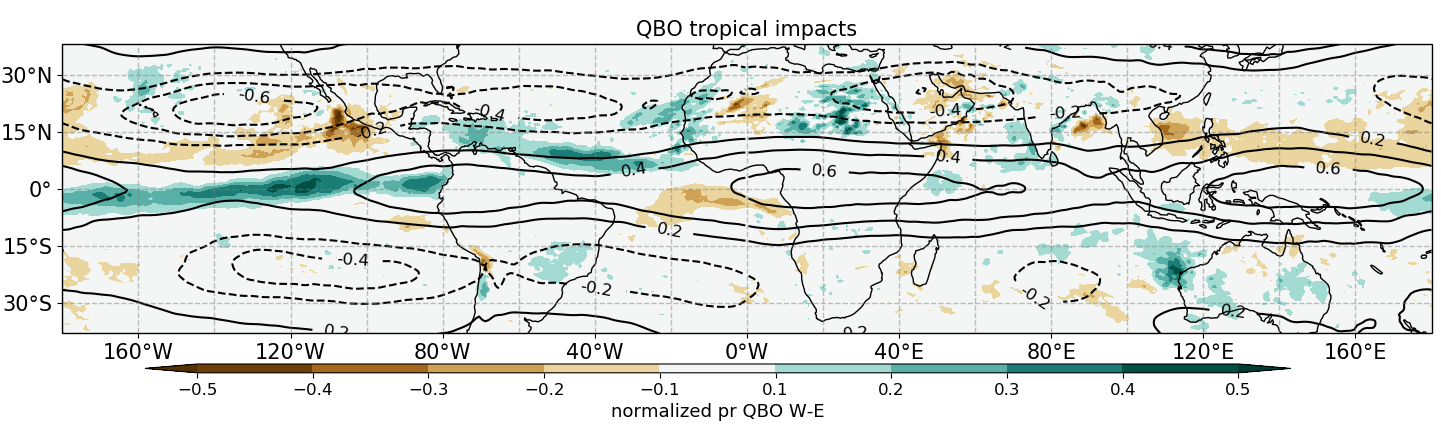
\includegraphics[width=\linewidth]{figures/finalfig.png}
\caption[Precipitation and 100 hPa temperature differences ]{QBO W-E annual-mean differences in air temperature at 100 hPa (contours) and precipitation normalized by the climatological values (shading) for the GC3 N216-pi simulation. }
\label{fig:qbo_mechanisms}
\end{figure}

Several different interpretations of the results from these CMIP6 pi-control and nudging experiments are possible. First, the disappearance of the surface response when the QBO nudging is introduced could suggest that there is no downward tropical route of the QBO. Similar discussions have arisen regarding the apparent MJO-QBO relationships, with some studies suggesting that there is no causal link, and that the observed relationship is a result of statistical effects \citep{wang2019}. 

Examination of the individual ensemble members of the 35-year coupled ocean experiments shows substantial variability in the surface precipitation response to the QBO in both the control and nudged experiments, which suggests that additional ensemble members would be desirable. However, the PDF in Figure \ref{fig:iod_suites}d for the IOD QBO singal, demonstrates that the results from the nudged ensemble members fall outside the variance caused by internal variability in the 500-years of the piControl simulation. Moreover, our analysis of 3 CMIP6 pi-control simulations each of >500 years suggests that a chance occurrence of the surface QBO signal in modelled precipitation is unlikely to be the case.  

Even accepting that the QBO signal in modelled precipitation is a real feature and not a statistical artifact, the results of the nudged experiments suggest that the signal is unlikely to be due to a direct downward influence of the QBO over the convective scheme of the model. The nudged AMIP experiments demonstrated that the QBO signal in SSTs was the primary cause of the precipitation signal and the direct QBO modulation of the upper tropospheric circulation was secondary to this. This conclusion is supported by further examination of the proposed UTLS static stability mechanism as 
the causal pathway through which the QBO influences the tropical troposphere.

 Several lines of evidence in this chapter seems to contradict the UTLS static stability mechanism. For instance, results from the first part of the chapter show zonally asymmetric responses that appear in all seasons, with much larger impacts over ocean than over land.  If the UTLS static stability mechanism was a dominant process, then one would expect that the QBO signal should produce zonally symmetric effects or at least an impact over all regions of deep convection since there is no reason why land monsoon regions 
should be less affected. 

Using results from the 500-year GC3 N216-pi  experiment, Figure \ref{fig:qbo_mechanisms} shows that the QBO W-E differences in 100 hPa temperature are not well co-located with the surface precipitation differences. In South America and Africa, there are large differences in the 100 hPa temperatures but little corresponding differences in precipitation, whereas the Central Pacific shows a similar UTLS temperature signal and a stronger precipitation signal. Therefore, this suggests that even in the free-running simulation, the proposed UTLS static stability mechanism is unlikely to be the dominant influence. 

Evidence against this mechanism appears to be even more apparent in the nudged experiments, where the QBO-related variations in UTLS static stability are larger than in the free-running model experiments but the surface responses have disappeared entirely. 
Another plausible explanation is that the convective scheme in the model is not sensitive to the static stability variations associated with the QBO \citep{yamazaki2020tropospheric}. This means that although the static stability mechanism may still be relevant in the real-world, our results suggest that within a state-of-the-art GCM the dominant factor has to be another process.

In summary, this chapter has shown that robust links exist between the QBO and the 
tropical troposphere in a state-of-the-art climate model. The modelled QBO signal in tropical precipitation compares well with the QBO signal in GPCP observations. Experiments in which the QBO zonal winds were nudged towards ERA5 reanalysis winds clearly demonstrated that the precipitation signal is a response to QBO variations in the SSTs rather than a direct downward teleconnection from the stratosphere, for example via modification of the static stability. Nevertheless, the origin of the QBO signal in SSTs is unclear and research is required to further explore this signal.


For example, the results of the 500-yr CMIP6 simulations suggest the possibility of a more subtle QBO influence that depends strongly on the phase of ENSO. The analysis showed that DJF seasonal interannual differences can depend both on ENSO and the QBO, as well as an interaction between QBOW / El Nino and between QBOE / La Nina, leading to asymmetric frequencies of ENSO events.
 If the QBO influence is non-linear as this suggests, so that a positive QBO-SST feedback only operates during modest-to-strong ENSO events (for example if the QBO feedback is sensitive to the longitudinal position of the Walker circulation), then imposing a fixed QBO evolution via the nudging scheme is likely to break this feedback loop. Further model analysis to explore this non-linear relationship in our model experiments e.g. whether the amplitude of the extreme ENSO events is reduced in the nudged experiments would be of interest, although the relatively infrequent occurrences of ENSO extremes may make it challenging to obtain a statistically significant result and more ensembles may be required.    
%This chapter has therefore proven that robust links exist between the QBO and the tropical troposphere in a state-of-the-art climate model.  
%Nevertheless, the results of this chapter are inconclusive as to the mechanisms that generate this coupling, as experiments with a nudged stratosphere remove these links.  If there is no downward stratospheric-tropospheric teleconnection, further research must explain why some robust sensitivity to the QBO phase appears in the model for several convective features. 

%For example, why is the ENSO index more frequently positive under QBOW, given that the ENSO has little-to-no effect over the descent rates and amplitude of the QBO \citep{serva2020} in this model. 
%Further work is needed to investigate what mechanisms explain the robust relationships found in various model configurations, some of which remarkably match observations, in this chapter. Suggestions for future research directions are given in the next chapter.

% \added{Rather, our results support the hypothesis that the links between the QBO and the Walker circulation best explain the characteristics of the responses \citep{hitchman2021observational}. One could reasonably assume that a robust local effect over the Maritime continent, for instance the UTLS static stability hypothesis, would then influence the strength of deep convection in the ascending branch of the Walker circulation and thereafter propagate to the rest of the tropical atmosphere. However, there is no way of identifying the causal pathways of this stratospheric-tropospheric coupling without targeted model experiments.  }
%The position of the East Pacific and Atlantic ITCZs is significantly different between the two phases of the QBO in the three experiments; however, the season of strongest influence varies for each model. 
%For example, the southward displacement of the East Pacific ITCZ in QBOW compared to QBOE phases  \citep[as previously reported, e.g., by][]{gray2018} is confirmed but in GC3 N216-pi this shift of the ITCZ is strongest in MAM whereas in GC3 N96-pi the most pronounced shift is in the DJF season. 
%The position of the Atlantic ITCZ is found further  northward during QBOW than during QBOE periods in all the simulations; the strongest response is found during late boreal spring and early summer in UKESM-pi. 

%In addition to multiple lines of observational and modelling evidence that suggest an influence of the QBO over tropical convective phenomena, results from Chapter \ref{ch:4-ams} showed that the impact of ENSO on the Walker circulation and associated teleconnections was sensitive to the phase of the QBO in the CMIP6 experiments of the MOHC and this chapter follows up on that evidence. 
%The first part of the chapter analyses CMIP6 experiments that reasonably simulate the QBO features, and the second part of the chapter describes and reports the results of simulations realized with MOHC models in which the equatorial stratosphere was relaxed towards an observed state.
%
% First, the chapter describes the annual and seasonal mean surface response of precipitation to the two phases of the QBO in the CMIP6 pre-industrial control experiments: UKESM-pi, GC3 N96-pi, GC3 N216-pi.  
%Results in the models generally agree with the results documented in observational studies \citep{liess2012,gray2018} and with the observational and reanalysis datasets employed throughout this thesis. In particular, the most robust impacts are observed over the ocean, particularly over two coupled ocean-atmosphere phenomena: the East Pacific and Atlantic ITCZ and the IOD. 

%For most land-monsoon regions, little evidence was found of robust impacts on the local summer monsoon precipitation associated with the QBO, in spite of observations from satellite-derived and gridded station data suggesting otherwise \citep{collimore2003,liess2012,gray2018,lee2019}. For example,  the South American monsoon region exhibited different responses in eastern Brazil than in the southernmost part of the monsoon. The surface response over land also varied notably from model to model.
%One hypothesis for the lack of a spatially coherent signal over land is the differences in the representation of the monsoon dynamics and feedbacks between the three models UKESM-pi, GC3 N96-pi, GC3 N216-pi that may represent the land-surface processes and moisture transport differently, so that any grid-scale impact of the QBO on the convective profile may produce different dynamic responses in the lower troposphere. 
%
%The influence of the QBO over the Indian and Pacific Oceans was confirmed through multi-variate regression analysis, suggesting an independent effect of the QBO from ENSO in these ocean basins. 
%However, the QBO-related differences over the Atlantic and East Pacific ITCZ appear to also depend on the phase of ENSO, suggesting a non-linear interaction between the ITCZs, ENSO and the QBO which may be confounded when using regression analysis.  
% The observed relationship between the QBO and ENSO is confirmed in this chapter in the CMIP6 experiments, as more frequently El Niño events appear during QBOW than during QBOE and the opposite for La Niña. 
% 
% A zonal gradient of convective precipitation in the Indian Ocean appeared in all the simulations, and this signal maximised during SON. 
% This zonal gradient was further diagnosed through an index that was found to be significantly sensitive to the QBO  phase, the index was found to be positive during QBOW and negative during QBOE, indicative of wetter conditions in the western Indian Ocean than in the eastern  Indian Ocean during QBOW and the opposite during QBOE. To our knowledge, these results are the first suggestions of a surface impact of the QBO associated with the IOD during SON.
% 
%Observational evidence has found coupled ocean-atmosphere interactions between the IOD, ENSO and the tropospheric quasi-biennial oscillation (TBO), which is a variation of weak-to-strong monsoons with similar periodicity to the stratospheric QBO \citep{meehl2003,pillai2010}. 
%This evidence could possibly explain these modelling results suggesting a link between the QBO, the IOD and ENSO simply by aliasing the QBO with the TBO signal.
%However, the period of the QBO in UKESM1 and HadGEM3 is longer than in observations, specifically 37-40 months for UKESM1 and 30-34 months for HadGEM3, which means the aliasing with a TBO in the model is unlikely.
%
% The zonal asymmetry in the QBO surface impacts in the tropics documented in observations \citep{collimore2003,liess2012,gray2018,lee2019} is also observed within these simulations. 
% Regional effects that depend on the longitude suggest that there is not a clear single effect of the QBO over precipitation, in contrast to early suggestions \citep{gray1984} that in general more precipitation would be observed during one phase of the QBO. 
% This chapter demonstrates that the relationship between the QBO and tropical convection is not likely only relevant at the grid-box scale, but the large and regional scale dynamics in the tropics are very important and thus QBO responses appear zonally asymmetric.
% 
% The hypothesis that the QBO may influence the mean-state of the Walker circulation suggested by previous observational studies to explain zonally asymmetric responses \citep[e.g.][]{collimore2003,liess2012} is confirmed as the Walker circulation varies by up to 10\% between QBO phases, even when the effect of ENSO events is taken into account. 
% Specifically, the Walker circulation is found to be weaker during QBOW than during QBOE. In DJF, this anomaly of the overturning circulation in the Pacific is likely linked to the East Pacific ITCZ shifts, and in SON, the changes to the overturning are likely linked to the ascending and descending motions in the Indian Ocean that generate the IOD response documented in this chapter.
% 
%The relationships found between the QBO, the Walker circulation and ENSO frequency could potentially be causally linked with the QBO variability being the driving mechanism. Changes to the mean state of the Walker circulation are known to modify the frequency of El Niño events and La Niña events. A weaker state of the Walker circulation could more likely trigger an El Niño event during QBOW than during QBOE, and similarly, a stronger Walker circulation during QBOE could more likely trigger a La Niña event, which would be consistent with the results of this chapter. 
%
% 
% The results of this chapter are one of the few analyses of the tropical route of QBO teleconnections within a fully coupled GCM. 
% The length of the pre-industrial control experiments (500 yr) was useful to adequately evaluate the statistical significance of the relationships between the QBO and tropical climate features. 
%Furthermore, the fact that most of the impacts diagnosed in this chapter are very similar in the three simulations, despite their differences in resolution and inclusion of Earth System processes provides robustness to the results. Nevertheless, the dynamical core of all the simulations is the same, so the parametrisation schemes such as the convective and gravity-wave scheme are identical. Further work needs to evaluate these relationships in different models from CMIP6.
% 
% However, the direction of causality cannot be interpreted from the regression or composite analyses presented in this chapter. For example, the ENSO-QBO relationships could be explained by anomalous tropical wave activity associated with ENSO modifying the downward propagation of the QBO \citep{schirber2015} or alternatively, the QBO temperature variability affecting convection in various regions and modifying the tropical circulation. 
%Further experiments are needed to separate the mechanisms that could explain these relationships and that could separate the directions of influence between the tropical stratosphere and troposphere. 
% 
% % however the direction of causality could not be addressed in this part of the chapter, which leads into the second part of the chapter.
% 
% %\end{document}


%\section{The case for nudging}
%
%
%
%Global climate models exhibit a number of biases in their representation of various aspects of the climate, all of which lead to uncertainty in our ability to make statements about the real-world based on their results. One example of a key bias discussed in this thesis is the magnitude and position of precipitation associated with the ITCZ in the Atlantic Ocean, which is associated with biases in South American precipitation. % the mean state of the Pacific and Atlantic SSTs as well as many others. 
%For this section, one relevant bias to consider is how current models represent the tropical stratosphere and, in particular, their representation of the QBO.
%
%
%
%
%The number of GCMs with a full stratosphere have increased notably from CMIP3 to CMIP6 which means that features such as the QBO are increasingly better resolved with each iteration of the CMIP \citep{bushell2020,richter2020}. Nevertheless, several aspects of the QBO are still not well represented by state-of-the-art climate models, such as the period and amplitude of the QBO \citep{schenzinger2017,richter2020}. 
%These biases increase uncertainty in teleconnections diagnosed from these models, because these biases could make the models misrepresent processes that are observed in the real-world between the tropical stratosphere and troposphere.
%
%\begin{figure}[t!]
%\centering
% \noindent
% 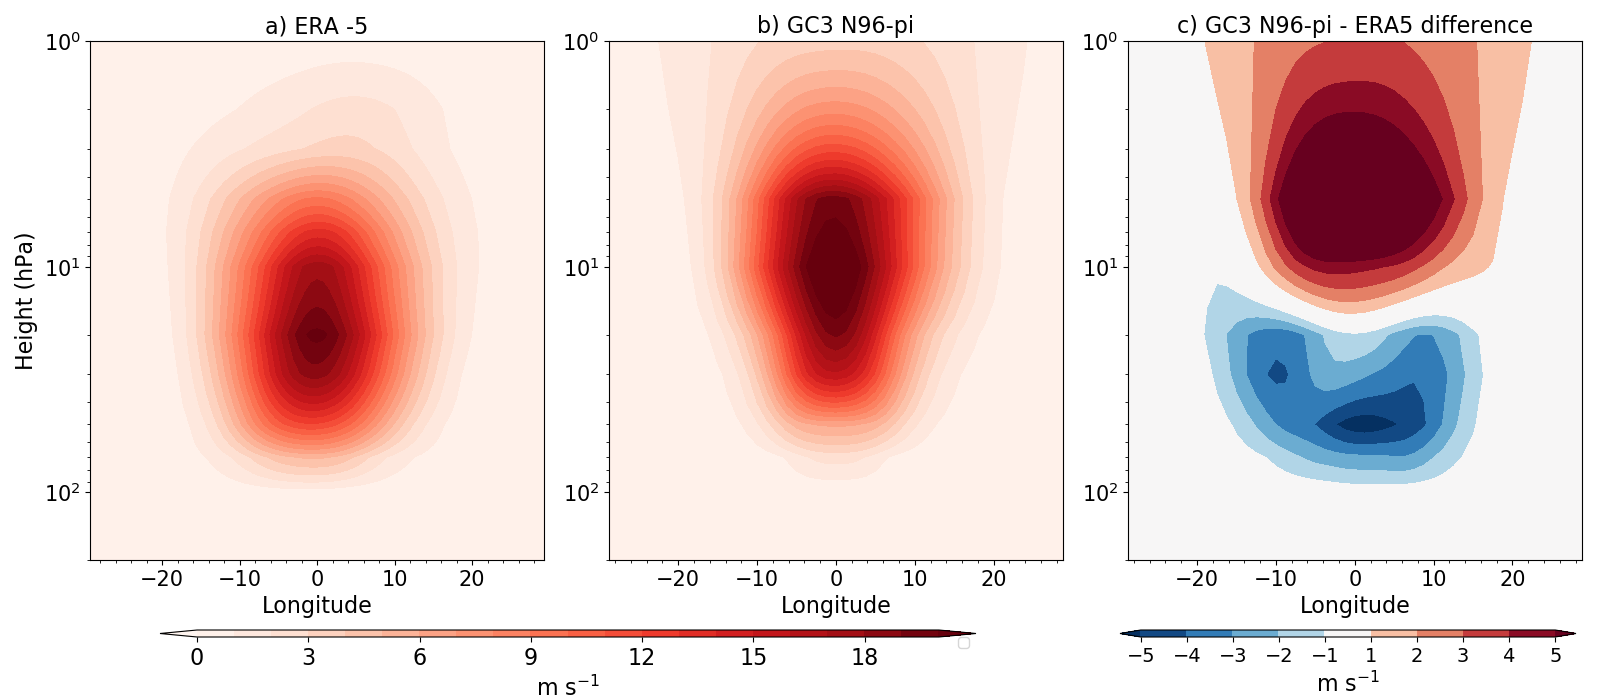
\includegraphics[width=\linewidth]{figures/qboamplitude.png}
%\caption[QBO amplitude bias]{Latitude-pressure plot of the amplitude [m s$^{-1}$] of the QBO. Obtained from the zonal mean zonal wind fourier spectrum magnitude within the QBO periods, as in \cite{schenzinger2017}. }
%\label{fig:qboamplitude}
%\end{figure}
%
%
%
%\section{ Results from nudging experiments}
%
%This section investigates the effect of nudging for the representation of the QBO, the variability in the upper troposphere lower stratosphere (UTLS) associated with the QBO, and ultimately, surface impacts driven by QBO effects on tropical convection. 
%First, this section evaluates how nudging modifies the wind and temperature variability in the UTLS region compared to control and CMIP6 simulations.  
%
%\begin{figure}[b!]
%\centering
% \noindent
% 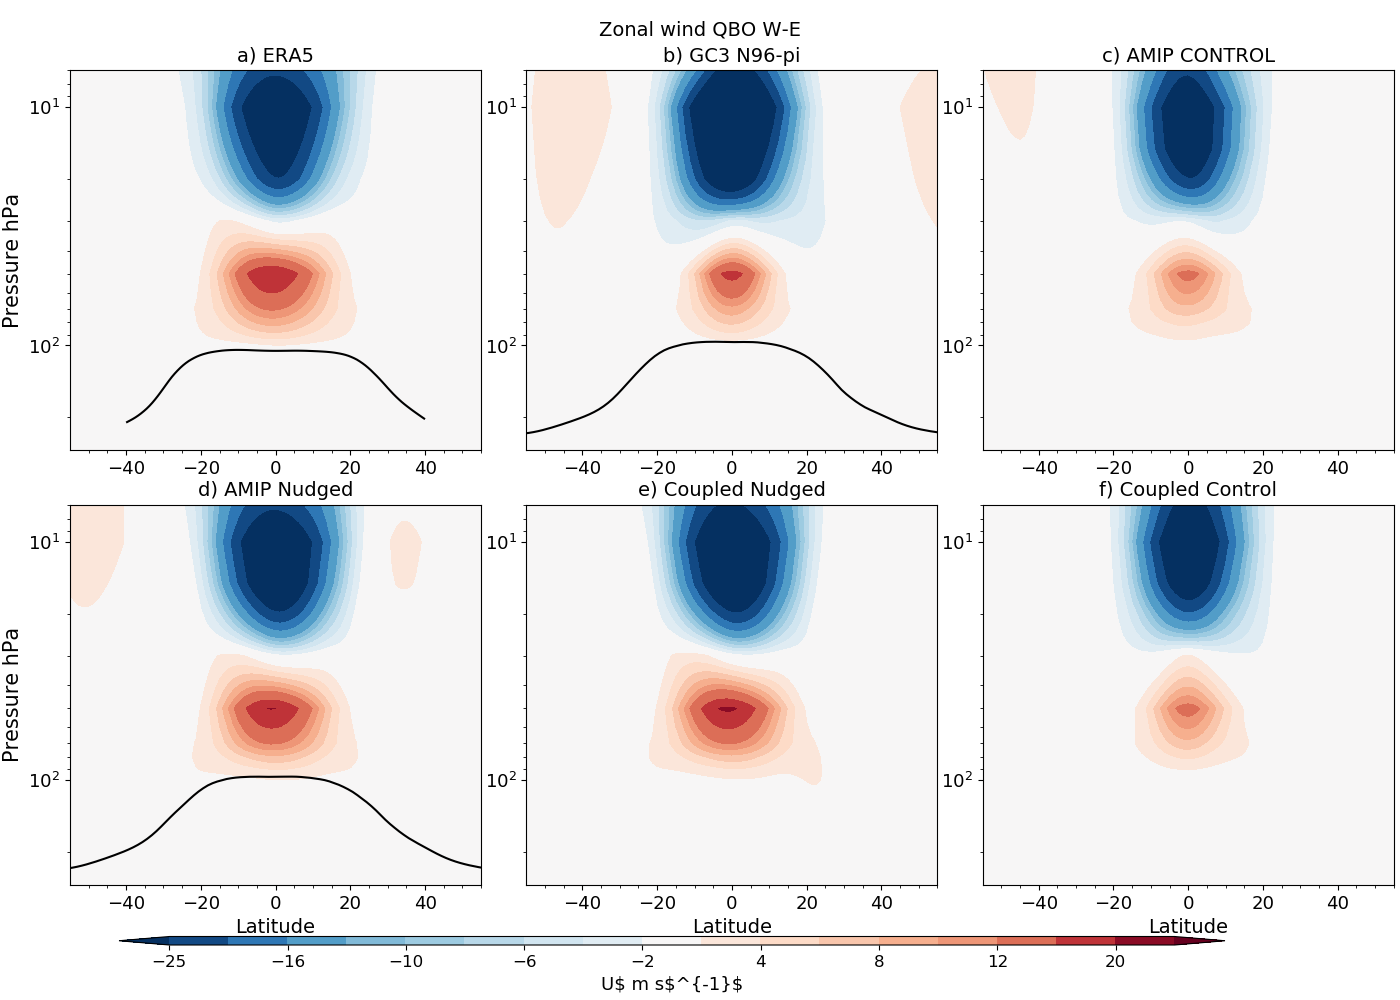
\includegraphics[width=\linewidth]{figures/zonalplotx_wind.png}
%\caption[Zonal mean zonal wind QBO difference]{Latitude-height plot of the zonal-mean zonal wind differences (QBO W-E) in (a) ERA5, (b) GC3 N96-pi from CMIP6, the control simulations with no nuding in an (c) AMIP and (f) coupled configurations, and the nudged simulations in (d) AMIP and (e) coupled configurations. The black line denotes the tropopause height obtained from the model data in (b, d) and for ERA5 the tropopause height was found through the gradient threshold method. For the nudged experiments, the ensemble-mean is shown. }
%\label{fig:zonal_u}
%\end{figure}
%
%
%\subsection{Tropical UTLS variability}
%
%
%Figure \ref{fig:zonal_u} shows that the zonal mean difference in zonal wind associated with the QBO phase, in a latitude-height sense, is deficient in the GC3 N96-pi and control experiments, principally near the tropopause as the signal is too narrow and weaker than in the reanalysis.
% 
%\begin{figure}[b!]
%\centering
% \noindent
% 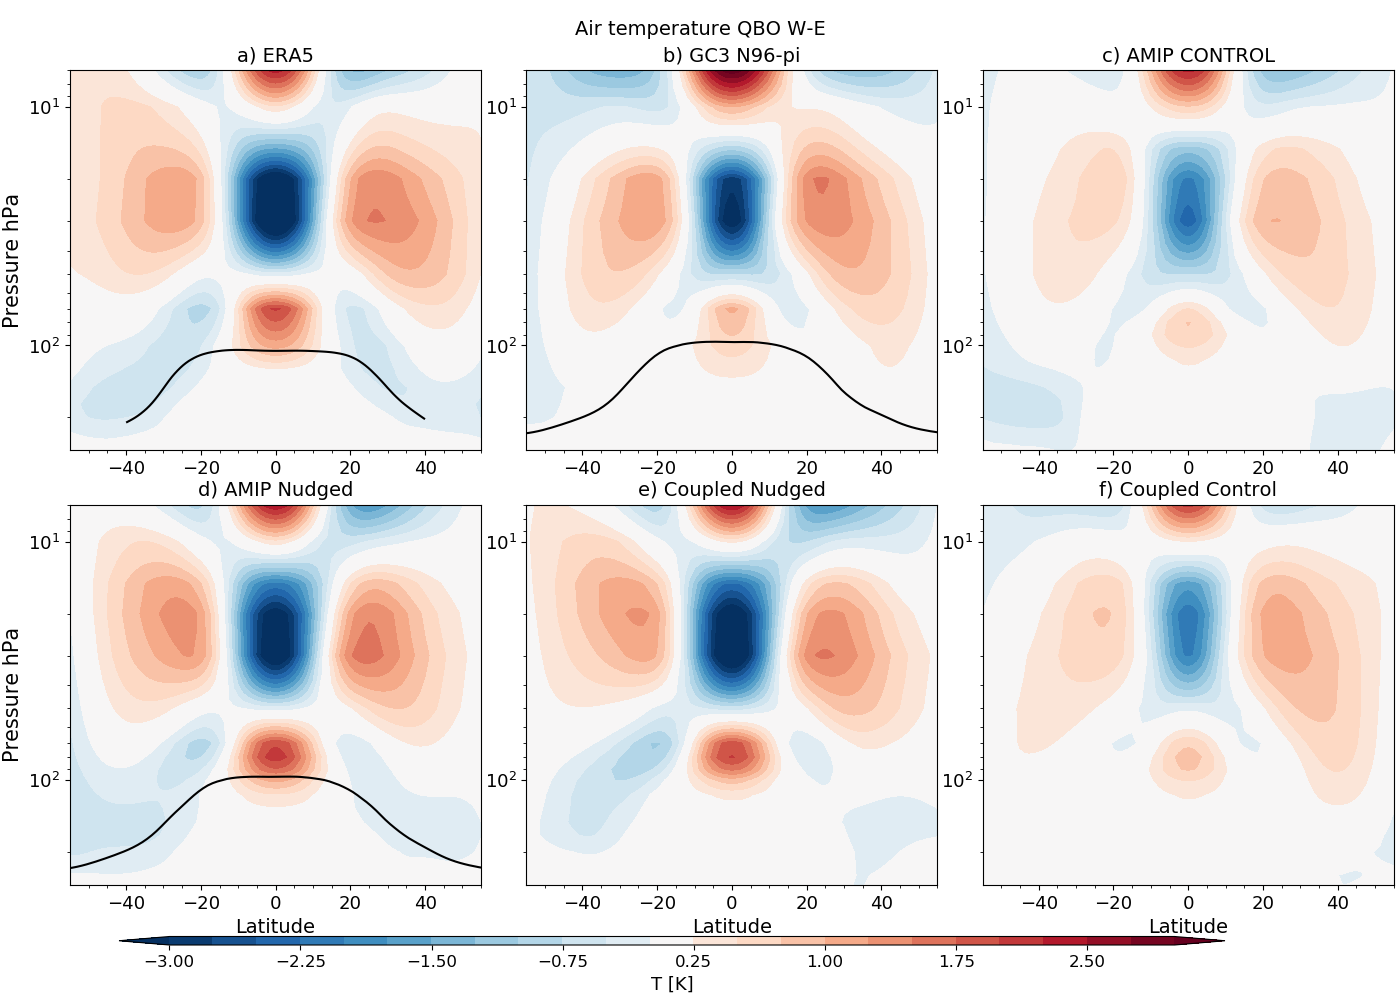
\includegraphics[width=\linewidth]{figures/zonalplotair_temperature.png}
%\caption[Zonal mean air temperature QBO difference]{As in Figure \ref{fig:zonal_u} but for air temperature.  }
%\label{fig:zonal_T}
%\end{figure} 
% 
%The nudging technique improves the zonal wind signal notably by replicating the result observed in ERA5, as expected since the nudging data is ERA5.  In the nudged runs, the wind signal near the tropopause extends poleward more than in the free-running control simulations and the peak positive anomaly found at around 70 hPa. The variability in the mid-stratosphere winds is also improved as the signal is wider reaching the subtropics. This means that the representation of shear, which modulates temperature as well, is improved with the nudging in the 20$^\circ$S-20$^\circ$N.
%
%
%
%The temperature is able to respond to the nudging within the model freely, Figure \ref{fig:zonal_T} reveals that nudging the zonal wind can also improve the air temperature variability in the lower stratosphere driven by the QBO shear. The positive temperature anomaly in the equatorial region around the 100 hPa at the tropopause level is much weaker in the GC3 N96-pi, AMIP Control and Coupled Control compared to the two nudged experiments and to ERA5. The Nudged experiments not only improve the temperature signal in the equatorial lower stratosphere but seem to overestimate this signal around the 70 hPa level. Furthermore, observations show a horse-shoe temperature anomaly pattern in the subtropics characterised by a negative anomaly that extends from 20-40 degrees north and south, a signal that is missing in the GC3 N96-pi, AMIP Control and Coupled Control experiments but is recovered in the Nudged experiments. This means that without nudging further away than 20 degrees north or south, the subtropical signal is obtained by improving the residual circulation associated with the QBO. 
%
%\begin{figure}[t!]
%\centering
% \noindent
% 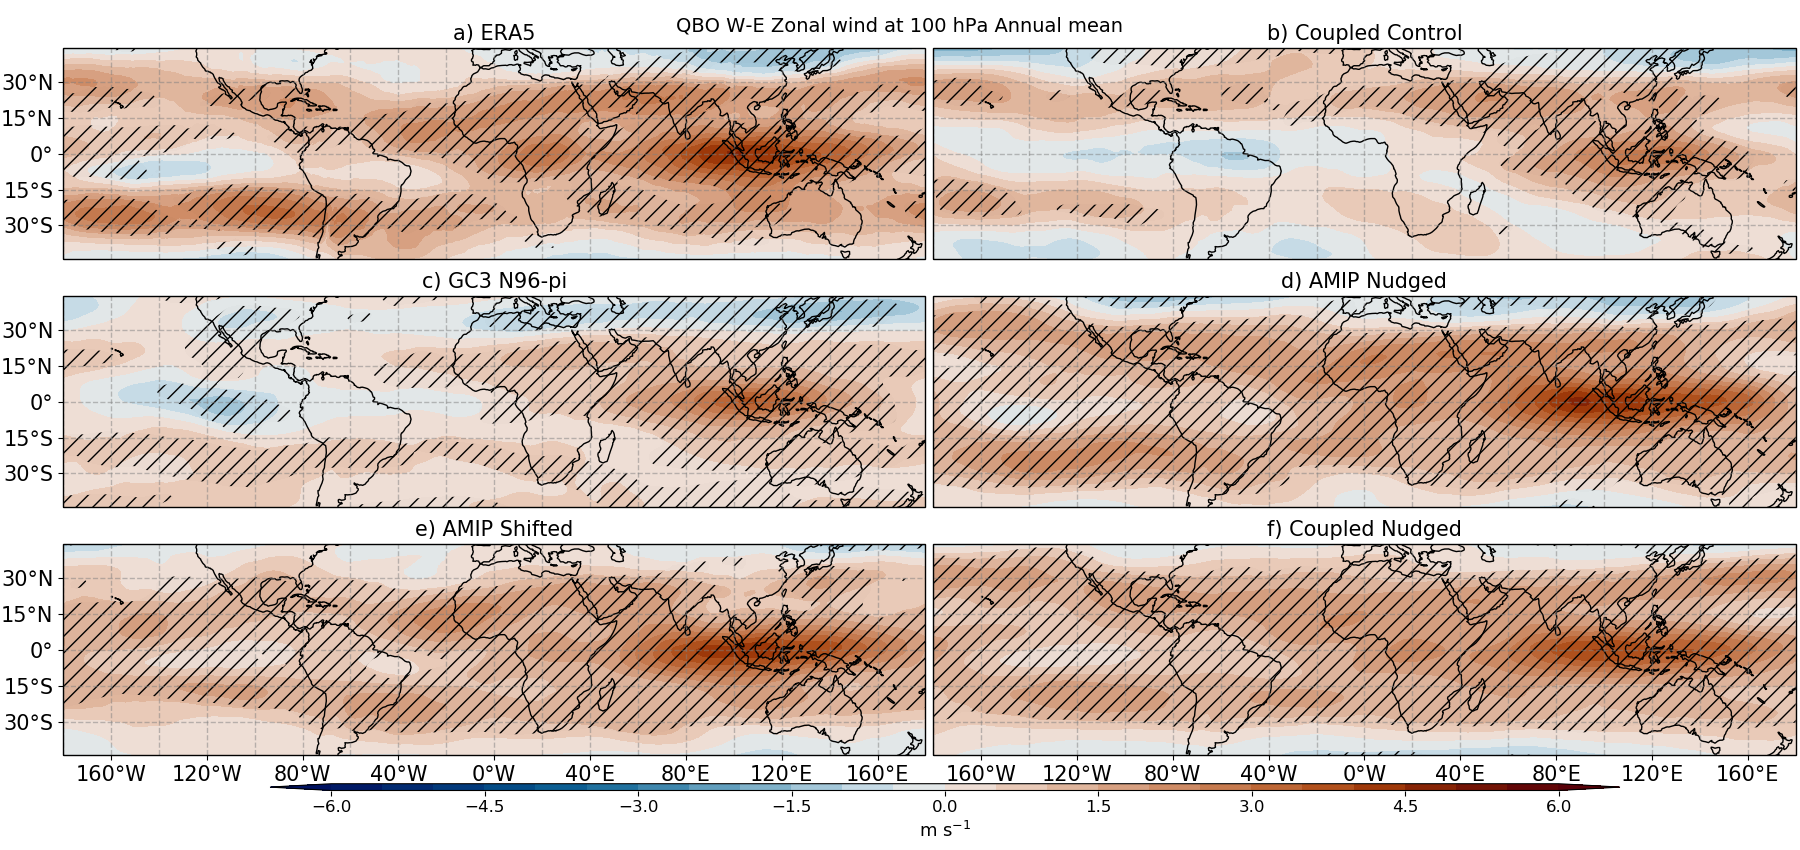
\includegraphics[width=\linewidth]{figures/ua100climqbowf.png}
%\caption[Zonal wind QBO W-E difference 100 hPa level]{Zonal wind difference in QBO W-E at the 100 hPa level. Hatching denotes significance to the 95\% level according to a Student's t-test.}
%\label{fig:ua100qbo}
%\end{figure}
%
%The spatial distribution of the wind and temperature variability associated with the QBO near the tropopause level (100-hPa level) is shown in Figures \ref{fig:ua100qbo} and \ref{fig:ta100qbo} for ERA5, GC3 N96-pi and control and nudged experiments. 
%These Figures show, first, that the free running model (seen in GC3 N96-pi and Coupled Control) is able to reproduce the zonal asymmetries in the QBO signal \citep{tegtmeier2020b} at the 100 hPa level albeit much weaker than the observed signal. The wind differences, for instance, is stronger in the Maritime continent in observations whereas the temperature signal is stronger in the Maritime continent equatorial Africa, both features reproduced sensibly by the model without nudging. 
%
%The nudging increases the magnitude of these signals at the 100 hPa level, both for the zonal wind and the temperature differences. Specifically, the temperature signal in the Nudged experiments is improved in AMIP Nudged and AMIP Shifted experiments, indicating that these differences are not associated with the underlying SST field, rather with the QBO vertical wind shear, which has been improved by nudging. 
%Results found in this analysis also indicate that the tropopause height and temperature exhibits more variability associated with the QBO than in the free-running model (not shown). 
%
%
%\begin{figure}[t!]
%\centering
% \noindent
% 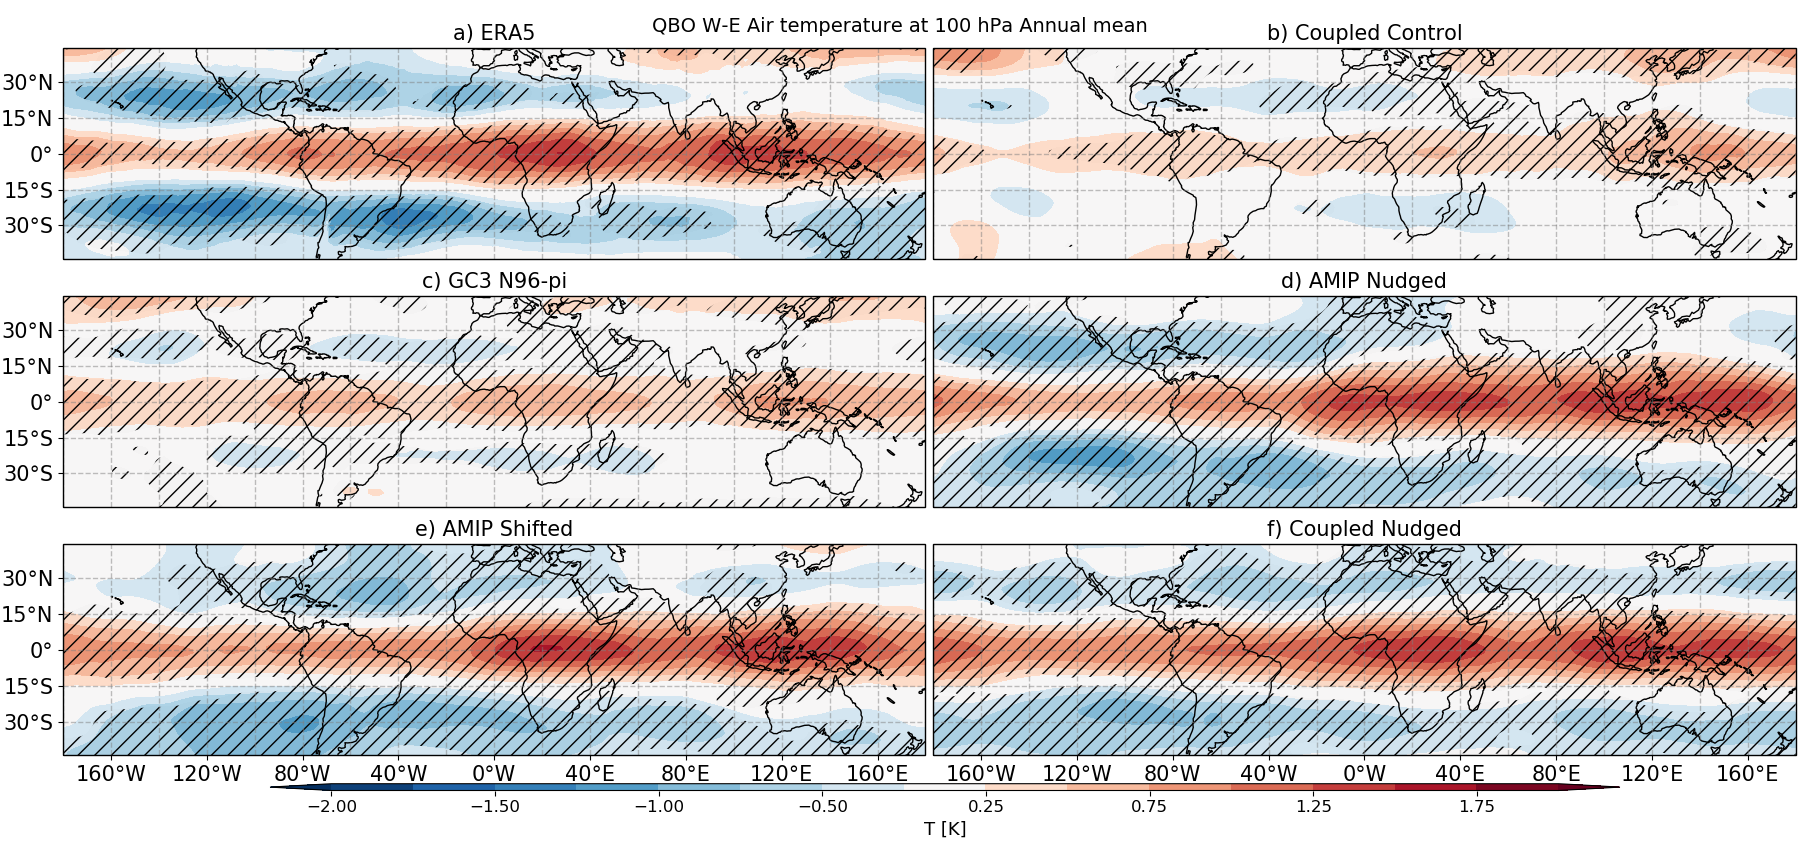
\includegraphics[width=\linewidth]{figures/ta100climqbowf.png}
%\caption[Zonal wind QBO W-E difference 100 hPa level]{As in Figure \ref{fig:ua100qbo}, but for air temperature. }
%\label{fig:ta100qbo}
%\end{figure}
%
%This section shows that the UTLS temperature and zonal wind variability are more realistic in the nudged experiments, and that this variability is not related to the underlying SSTs but rather a result of the relaxation in the equatorial stratosphere. These results indicate that these experiments are suited to investigate tropical teleconnections associated with the QBO. The hypothesis to test is that the processes that link the QBO to tropical convection should be more realistically represented in the nudged experiments than in the control experiments. %The following section investigates whether in fact surface impacts in the tropics are stronger in the nudged experiments compared to free-running simulations. 
%
%
%
%\subsection{Atmosphere-only experiments}
%
%This section describes the results of the atmosphere-only experiments: AMIP Nudged, AMIP Control and AMIP Shifted. These simulations use the CMIP6 SST dataset used for AMIP experiments, so that, in other words, the SSTs in these runs follow the observed seasonal and interannual variability of SSTs. 
%The effect of nudging on the tropical circulation is first described to evaluate whether nudging has significantly modified the mean state of the Hadley and Walker circulations. Then, the precipitation response to the QBO is compared between Nudged and Control AMIP simulations.
%
%\subsubsection{The tropical circulation}
%
%\begin{figure}[t!]
%\centering
% \noindent
% 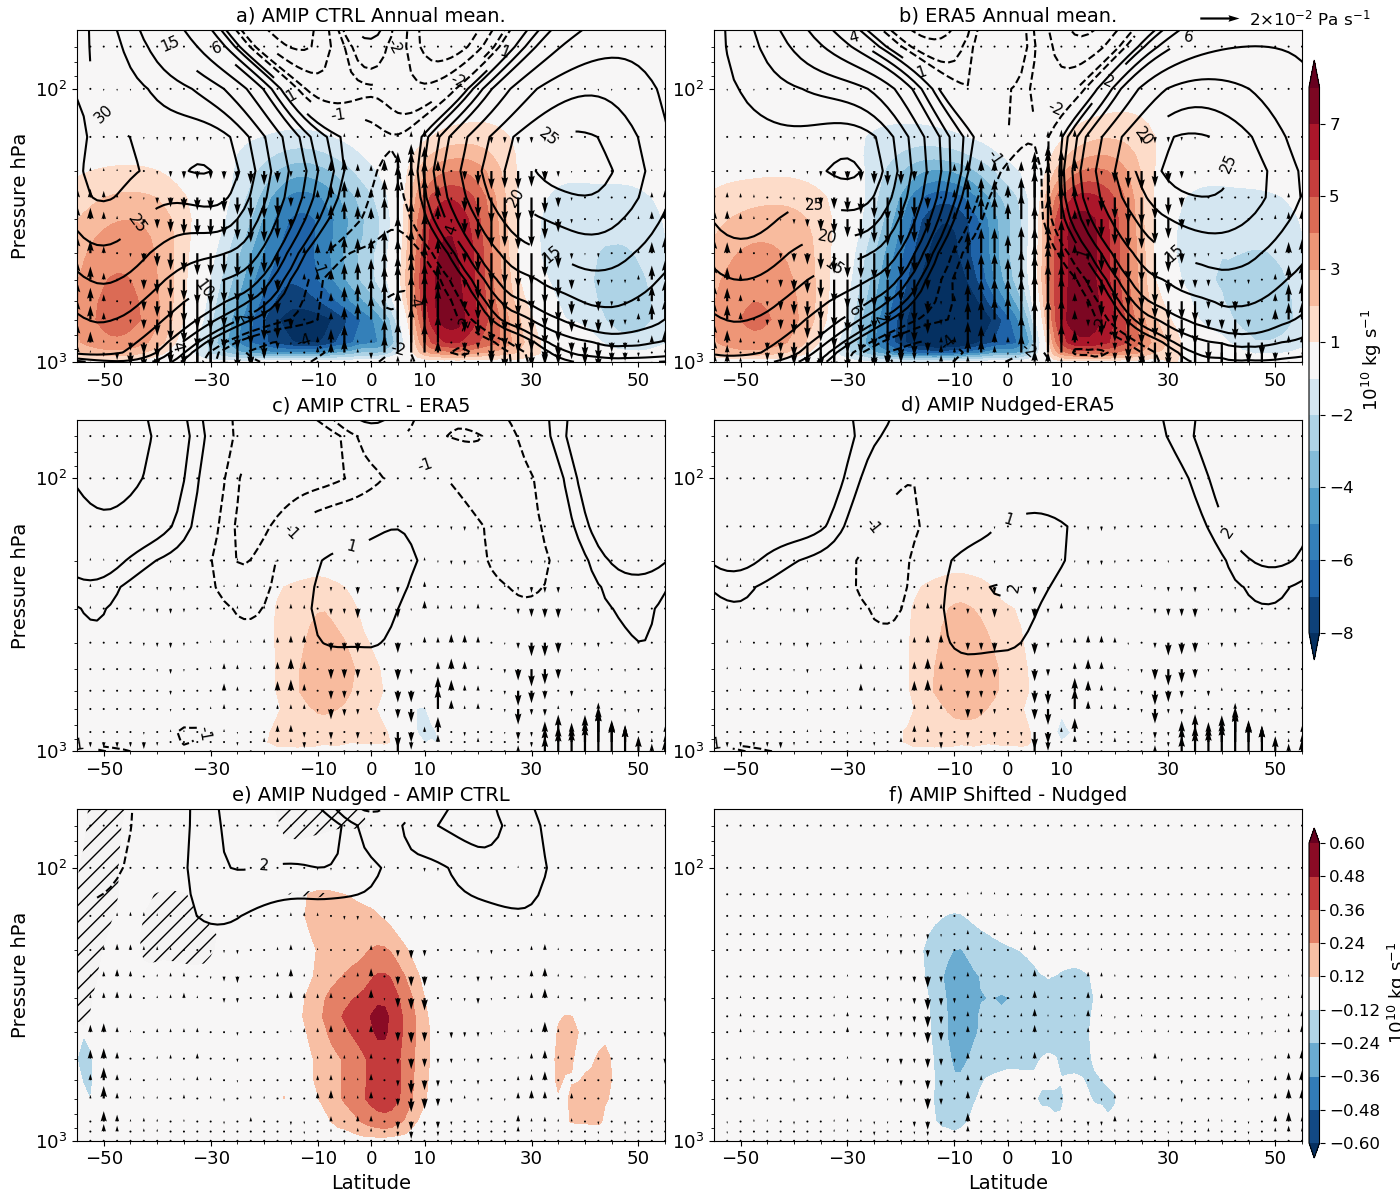
\includegraphics[width=\linewidth]{figures/suite_streamhadleyclim.png}
%\caption[Hadley cell in atmosphere-only experiments]{Hadley cell meridional mass streamfunction (shading), zonal mean zonal wind (contours) and vertical velocity (vectors). (a) Climatological mean in the AMIP Control experiment, (b) Bias in the Control experiment with respect to ERA5, differences between (c) AMIP Nudged-Control and (d) AMIP Shifted-Nudged. Note that the colorbar and scale of the vectors changes from the top to the bottom row. In (c-d), significant differences (95\% confidence level according to a Mann-Whitney two-sided test) in the streamfunction are highlighted with hatching . }
%\label{fig:hadleyamip}
%\end{figure}
%
%The mean state of the Hadley cell in the atmosphere-only configuration is weaker than in ERA5 in the 20$^\circ$S-0 region (the southern hemisphere branch in Figure \ref{fig:hadleyamip}) whereas biases in the upper-level tropical and subtropical troposphere, the model shows an easterly bias. 
%The AMIP Nudged simulation shows an improvement of this bias in the tropical and subtropical stratosphere showing positive zonal wind differences with the Control experiment in the UTLS region, i.e, correcting the easterly biases of the Control experiment. However, no significant differences in the streamfunction over the tropical troposphere are observed. Similarly, no significant differences were found in the mean-state of the Hadley circulation between the Nudged and Shifted experiments, suggesting that the variability of the nudging data is of secondary importance relative to the mean state of the nudging data. 
%
%\begin{figure}[t!]
%\centering
% \noindent
% 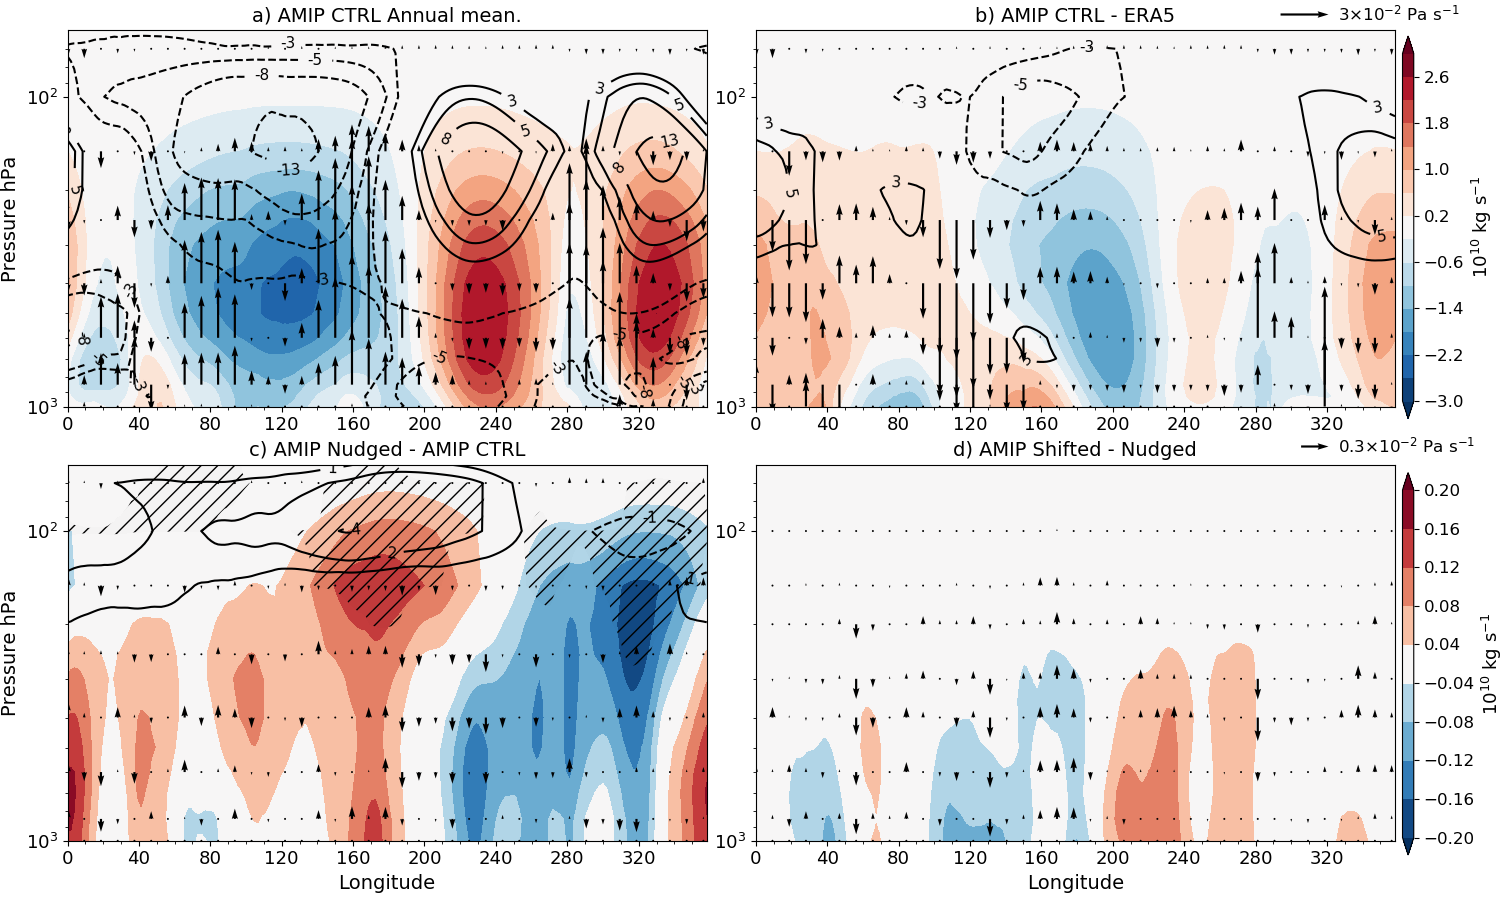
\includegraphics[width=\linewidth]{figures/suite_streamwalkerclim.png}
%\caption[Walker in atmosphere-only experiments]{Zonal mass streamfunction ($\psi$ in shading), zonal mean zonal wind (contours) and vertical velocity (vectors) averaged over the 10$^\circ$S-10$^\circ$N, as in Figure \ref{fig:hadleyamip}. }
%\label{fig:walkeramip}
%\end{figure}
%
%In turn, the Walker circulation biases in the upper troposphere are notably improved in the Nudged experiment (Figure \ref{fig:walkeramip}). The mean state of the Walker circulation is weaker in the AMIP Control simulation compared to ERA5, characterised by a weaker circulation in the Western Pacific and an easterly bias at upper levels. These two tropospheric biases in the Control experiment are reduced in the Nudged experiments, even though the relaxation is only applied above 90 hPa significant differences in the zonal wind and zonal streamfunction are observed at 200 hP near the dateline, over South America and over the Atlantic Ocean. 
%However, no significant differences are observed between the AMIP Shifted and Nudged experiments. 
%
%\begin{figure}[t!]
%\centering
% \noindent
% 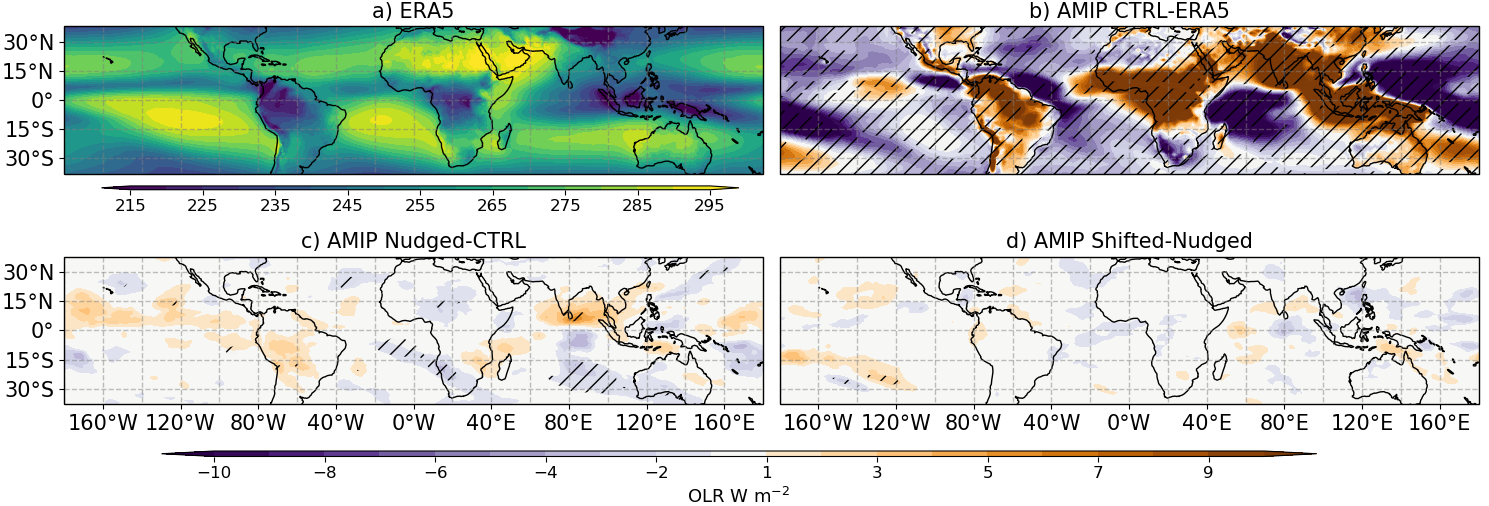
\includegraphics[width=\linewidth]{figures/olr_check.png}
%\caption[Annual mean OLR  in atmosphere-only experiments]{(a) Climatological mean OLR [W m$^{-2}$] in ERA5, (b) climatological biases in the AMIP Control simulation. (c) Differences between AMIP Nudged and Control and (d) between AMIP Shifted and Nudged. Significant (95\% confidence level) differences according to a Mann-Whitney U test in (c, d) are highlighted with hatching. }
%\label{fig:olr-mean}
%\end{figure}
%
%The mean state of the Hadley and Walker circulation at upper levels is modified in the simulations when nudging is applied, reducing the biases in the circulation within the model. However, these differences, or reductions of the biases, are smaller than the magnitude of the biases themselves, so it is unclear whether these differences are  large enough to improve other aspects of tropical climate. 
%
%\begin{figure}[t!]
%\centering
% \noindent
% 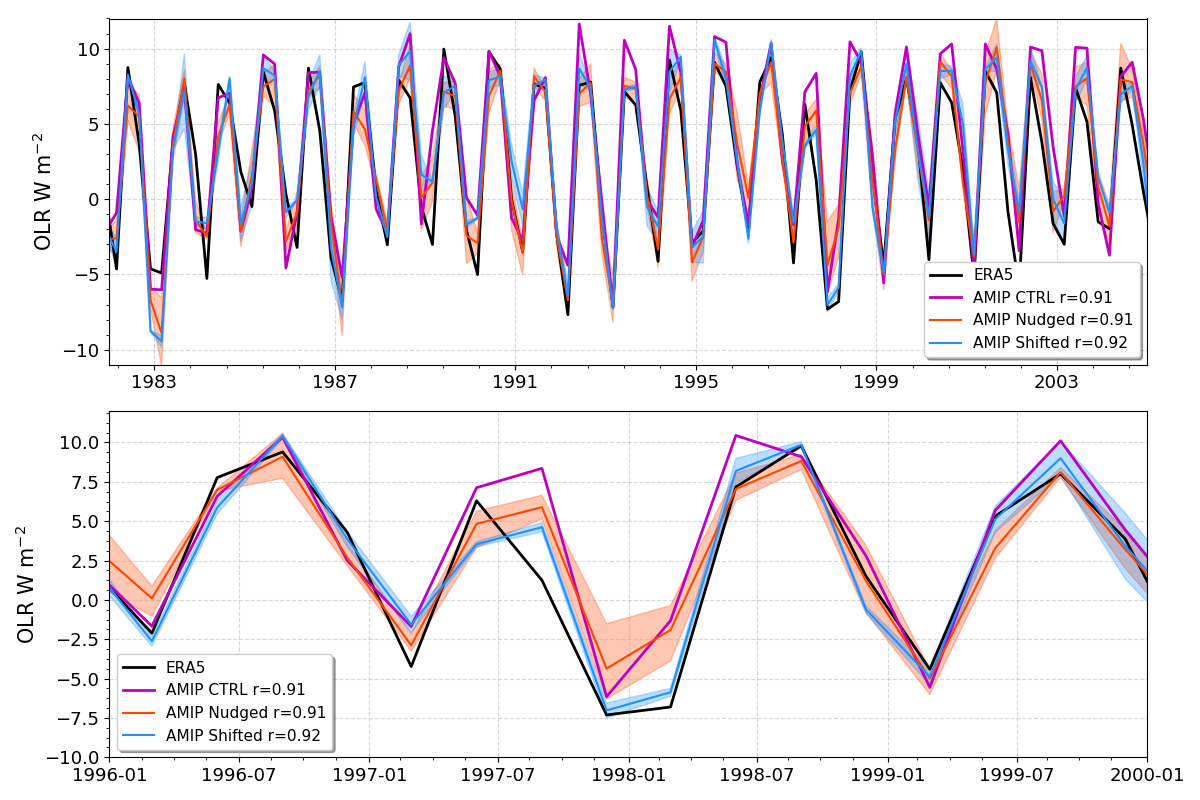
\includegraphics[width=\linewidth]{figures/olr_tseries.png}
%\caption[Tropical mean OLR time series.]{Time-series of zonal-mean equatorial [5$^\circ$S-5$^\circ$N]  OLR in ERA5 and the three amip experiments for (a) 20 yrs and a (b) 5-yr period around the 1997-1998 ENSO event. For each AMIP experiment the Pearson correlation coefficient between the experiment time-series and ERA5 is shown in the legend. }
%\label{fig:olramip_tseries}
%\end{figure}
%
%For example, Figure \ref{fig:olr-mean} shows the biases in the climatology of OLR, and the impact of Nudging on these biases. Most regions in the tropics exhibit significant and relatively large biases in AMIP Control compared to ERA5, most of which remain unchanged in the AMIP Nudged and Shifted experiments. The small and not significant differences between the two types of nudged experiments suggest a small effect of the relaxation of the zonal winds over the mean state of OLR. 
%
%Similarly, Figure \ref{fig:olramip_tseries} shows that the zonal-mean OLR time-series averaged over the deep tropics is undistinguishable between the three AMIP experiments, and the time-series of all the experiments have the same correlation coefficient with ERA5. In other words, the tropical mean OLR remains unchanged in the nudged experiments, regardles of whether the relaxation was implemented to match the SST field or whether the nudging data was shifted from the SST time-series. 
%Based on these results alone, it would appear that nudging has made little impact over the interannual variability of the tropical mean OLR. The question of whether the specific variability of OLR and precipitation associated with the QBO is also the same is now investigated in the next section. 
%
%
%\subsubsection{Precipitation response to the QBO}
%
%\begin{figure}[t!]
%\centering
% \noindent
% 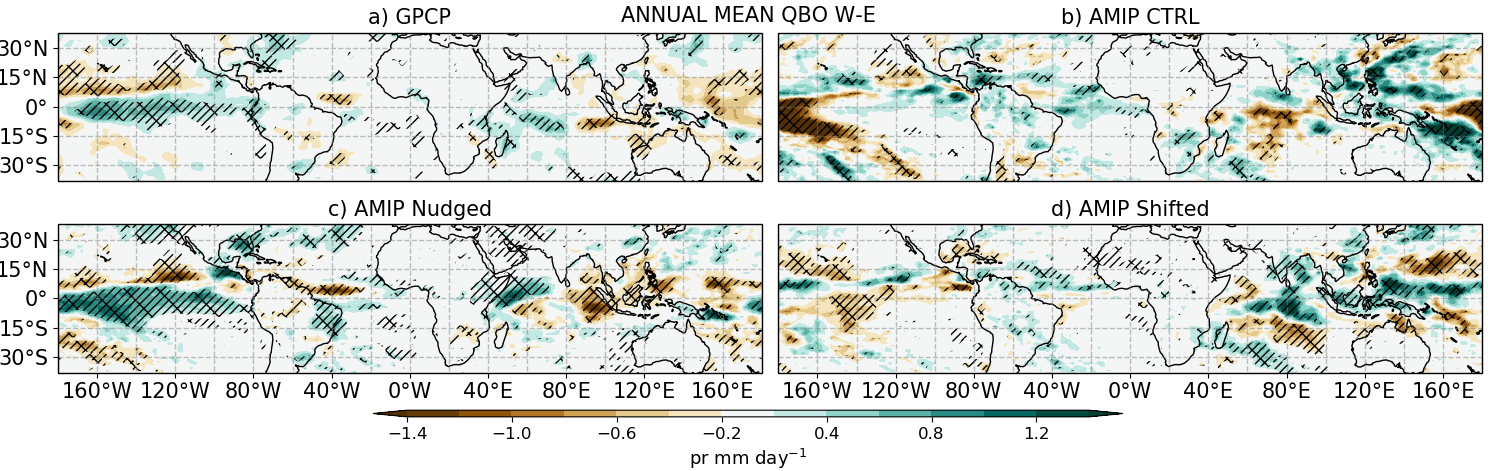
\includegraphics[width=\linewidth]{figures/pr_amip_climqbowqboe.png}
%\caption[Annual mean precipitation response in atmosphere-only experiments]{Annual-mean precipitation response (QBO W-E) in (a) GPCP, and atmosphere-only experiments: (b) AMIP CTRL, (c) AMIP Nudged and (d) AMIP Shifted.  }
%\label{fig:amip_clim}
%\end{figure}
%
%
%The annual-mean difference of precipitation between QBOWand E phases (Fig. \ref{fig:amip_clim}) in the ensemble-mean AMIP Nudged experiment matches closely the results of GPCP, characterised by an El Niño pattern in the Pacific Ocean, a weaker Atlantic ITCZ and a gradient of precipitation in the Indian Ocean during QBOW compared to QBOE. 
%In contrast, the free-running AMIP Control and the simulations with an out-of-phase relaxation of the winds with respect to the SST driving data (AMIP Shifted) show very different responses to the AMIP Nudged experiment and observations. 
%
%\begin{figure}[t!]
%\centering
% \noindent
% 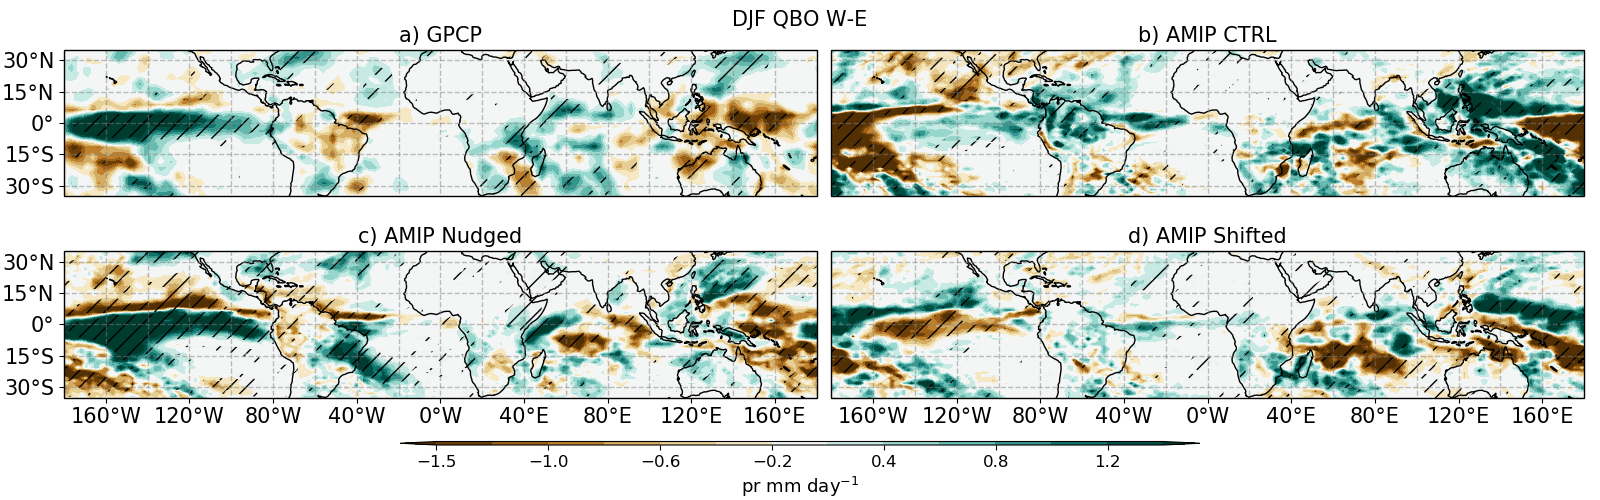
\includegraphics[width=\linewidth]{figures/pr_amip_djfqbowqboe.png}
%\caption[DJF mean precipitation response in atmosphere-only experiments]{As in Fig. \ref{fig:amip_clim} but for the DJF season. }
%\label{fig:amip_djf}
%\end{figure}
%
%A similar result is found when the composite differences only include DJF (Fig. \ref{fig:amip_djf}), so that the precipitation response in the simulations where the QBO index and the SSTs match exactly as in observations (AMIP Nudged) produce a very similar response to GPCP, whereas simulations where the QBO winds do not match the same SSTs result in different responses. 
%Results using OLR are very similar, for example, Figure \ref{fig:amip_son_olr} shows that a strong response is diagnosed in GPCP in the Indian Ocean which is reasonably reproduced in AMIP Nudged but AMIP CTRL and AMIP Shifted exhibit a very different response in the Indian Ocean and elswhere.
%
%
%
%These results suggest that the QBO winds are secondary to the effect of the SSTs for the precipitation response in these atmosphere-only experiments. The AMIP Shifted experiment has a better representation of the stratospheric variability in temperature and vertical wind shear, however, the response is entirely different to the AMIP Nudged experiments, the difference between these two experiments being the underlying SSTs. These results suggest that improving the representation of the QBO is not enough to replicate the observed response because the SST forcing dominates. 
%
%\begin{figure}[t!]
%\centering
% \noindent
% 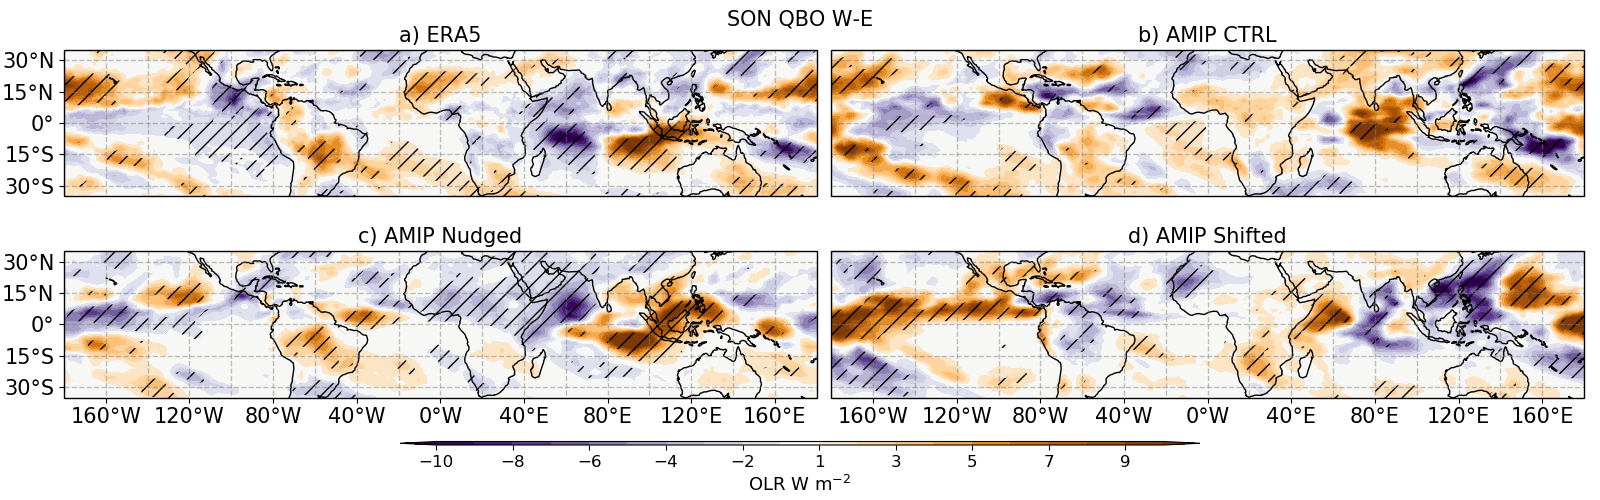
\includegraphics[width=\linewidth]{figures/olr_amip_sonqbowqboe.png}
%\caption[SON OLR response in atmosphere-only experiments]{As in Fig. \ref{fig:amip_clim} but for OLR in the SON season. }
%\label{fig:amip_son_olr}
%\end{figure}
%
%This section shows, first, that relaxing the zonal wind in the stratosphere in atmosphere-only experiments does not modify the mean state of the tropical circulation. Second, that the surface response of precipitation associated with the QBO in observations is largely associated with the underlying SSTs. The tropical mean OLR and precipitation mean state appear to be undistinguishable between Control, Nudged and Shifted experiments, whereas the composite differences between the two phases of the QBO reveal that the observed precipitation response is associated mostly with the SST anomaly pattern. However, whether the QBO has any effect over the SSTs cannot be answered in this atmosphere-only experiments, which leads to the the next section which analyses the coupled nudged experiments. 
%
%\subsection{Coupled experiments}
%
%
%This section presents the results of the coupled ocean-atmosphere experiments with (Nudged) and without (Control) relaxing the zonal wind in the tropical stratosphere. Note that all the individual experiments in this section are the same length (35 yr) and the Coupled Nudged ensemble-mean refers to the mean results of the six ensemble members with nudging.
%These coupled experiments differ only slightly from the setup used in the CMIP6 piControl experiments, analysed in section \ref{sq:cmip6_qbo}, with the atmospheric resolution of the nudged experiments matching the resolution of GC3 N96-pi and the oceanic resolution of these resolutions being the same of GC3 N216-pi. The forcing is constant in both types of runs, except that in the piControl experiments, the forcing represents conditions of the year 1850 and in the nudged experiments of the year 2000. 
%Due to these similarities, we compare the long-term CMIP6 experiments with the nudging experiments in some instances.
%
%\subsubsection{SST response}
%
%\begin{figure}[t!]
%\centering
% \noindent
% 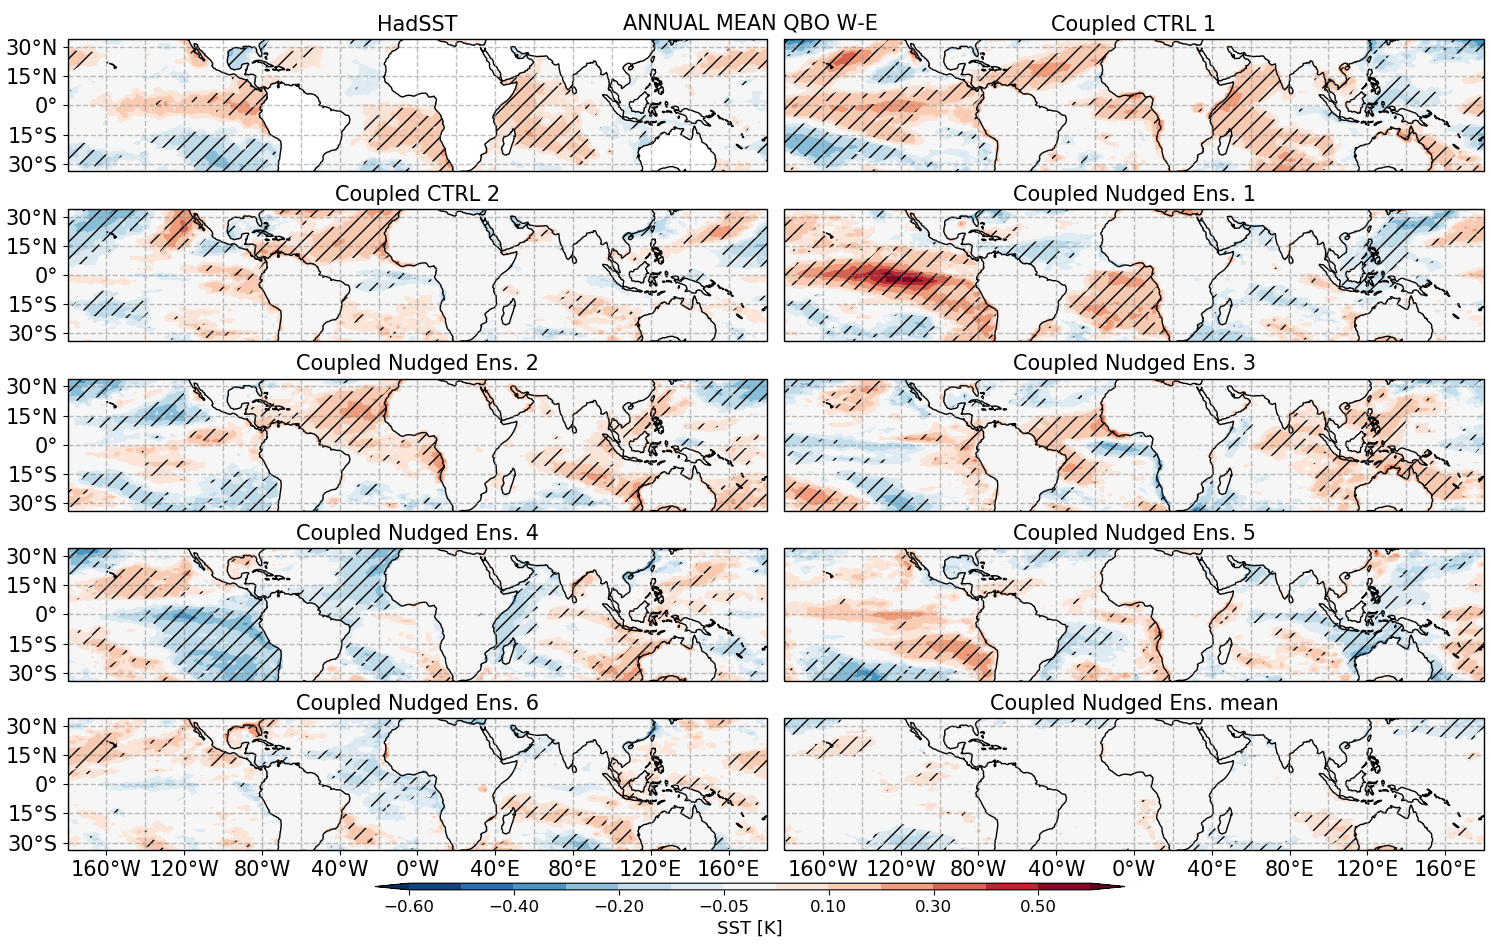
\includegraphics[width=\linewidth]{figures/sst_check_climqbowqboe.png}
%\caption[Annual mean SST response to the QBO in coupled nudged experiments]{ Annual mean SST [K] QBO W-E differences in the HadSST dataset and the Coupled Control, Coupled Nudged ensemble members and the Coupled Nudged ensemble mean. Hatching denotes significance to the 95\% confidence level according to a bootstrapping with replacement test.}
%\label{fig:sst_clim_coupled}
%\end{figure}
%
%
%The previous section shows that in atmosphere-only experiments the SST forcing dominates over any effect of the nudging, indicating that the mechanism by which the QBO influences tropical climate is involves the SSTs. In the coupled ocean-atmosphere experiments, the SSTs are able to respond and interact with any atmospheric forcing, and for that reason, this section first presents the annual mean and seasonal mean differences between the two phases of the QBO comparing coupled nudged and control experiments. 
%
%The annual mean difference in tropical SSTs between QBO phases in HadSST and each coupled experiment is shown in Figure \ref{fig:sst_clim_coupled}. In the HadSST dataset, the differences indicate a warmer East Pacific, and equatorial Atlantic and Indian Oceans. The first control experiment shows a very similar response in the Pacific and Indian Oceans whereas the results of the second control experiment only agree with the HadSST results in the subtropical North Atlantic and in the Western Pacific. 
%The nudged experiments, in turn, show a number of different responses, with differences being significant and positive in some regions in one ensemble and of another sign and unsignificant in other ensembles. 
%
%\begin{figure}[t!]
%\centering
% \noindent
% 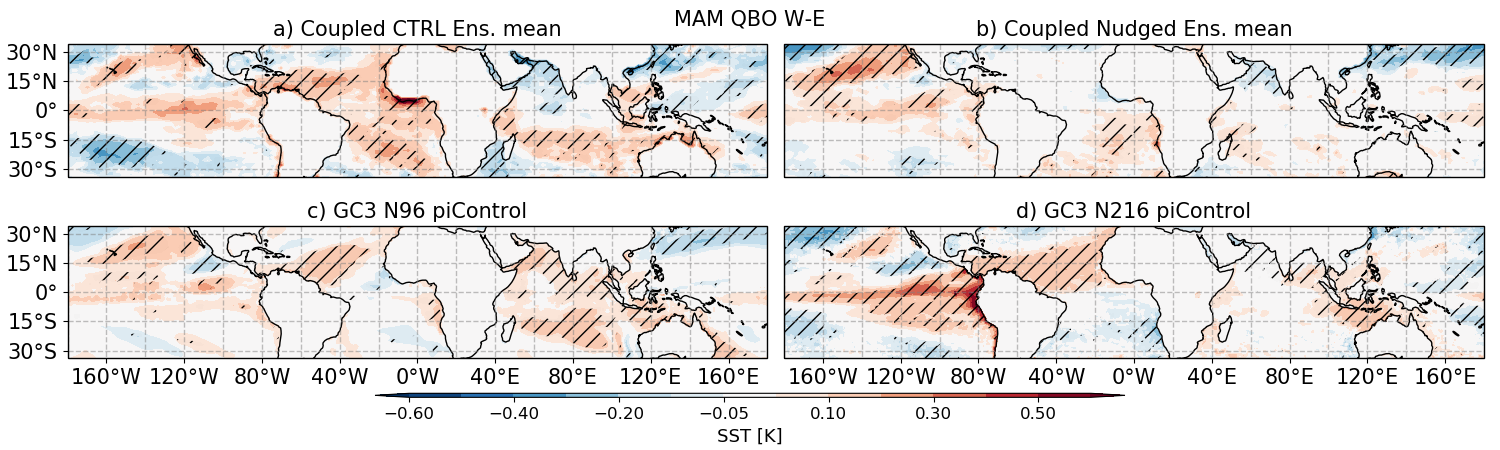
\includegraphics[width=\linewidth]{figures/sstseasonal_mamqbowqboe.png}
%\caption[SST response in MAM to the QBO in coupled nudged experiments]{ SST differences between QBO phases in MAM in (a) Coupled Control ensemble mean (2-member), (b) Nudged Coupled ensemble mean (6 members) and in the CMIP6 (c) GC3 N96-pi and (d) GC3 N216-pi.}
%\label{fig:sst_mam_coupled}
%\end{figure}
%
%The ensemble-mean response shows that averaging over all ensembles results in a weak mean response, with only some differences being different than zero and significant, for example the positive differences found over the coast of Australia and the subtropical Central Pacific. 
%In specific seasons, such as MAM (\ref{fig:sst_mam_coupled}), the SST response also appears to be stronger in the tropics in the free-running Coupled Control experiments than in the nudged experiments. 
%In MAM, a positive difference found in the Atlantic, Indian and Pacific Oceans in the CMIP6 experiments is also found in the control experiments but this response is weaker in the ensemble-mean of the nudged experiments.
%The nudged experiments show a relatively large difference in the eastern subtropical Pacific reaching the coast of California, in agreement with the control experiments.
%
%\begin{figure}[t!]
%\centering
% \noindent
% 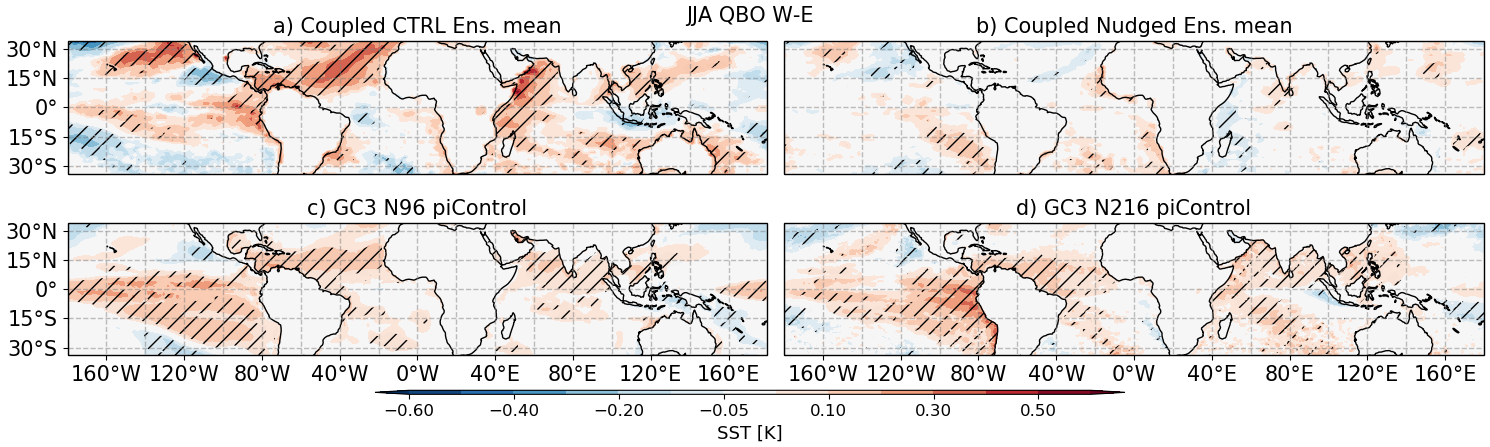
\includegraphics[width=\linewidth]{figures/sstseasonal_jjaqbowqboe.png}
%\caption[SST response in JJA to the QBO in coupled nudged experiments]{As in Fig. \ref{fig:sst_mam_coupled} but for JJA.}
%\label{fig:sst_jja_coupled}
%\end{figure}
%
%The pattern of positive anomalies in the equatorial Central and Eastern Pacific, as well as in the Atlantic Ocean, appears in the control and CMIP6 experiments in most months. 
%In boreal summer (Fig. \ref{fig:sst_jja_coupled}), the patterns are particularly strong in the Coupled Control ensemble mean in the Atlantic and Indian Oceans. However, the Nudged experiments show a very weak mean response in the tropics, only a warm difference found in the western coast of South America. 
%For the other seasons, SON and DJF, similar results are found (not shown) in which the ensemble mean of the control experiments agrees well with the CMIP6 experiments, whereas weaker responses are found in the nudged experiments.
%
%These results suggest that the SST response to the phase of the QBO in the nudged experiments is not significantly larger in the experiments compared to the control or the CMIP6 experiments, especially in equatorial regions. 
%In other words, the simulations with a stronger temperature signal associated with the QBO show the seemingly weakest response to the phase of the QBO.
%The lack of robust and large patterns of SST anomalies suggests that the precipitation response may also be weaker in the ensemble mean of experiments with nudging, which is the topic of the next section.
%
%\subsubsection{Precipitation response}
%
%\begin{figure}[t!]
%\centering
% \noindent
% 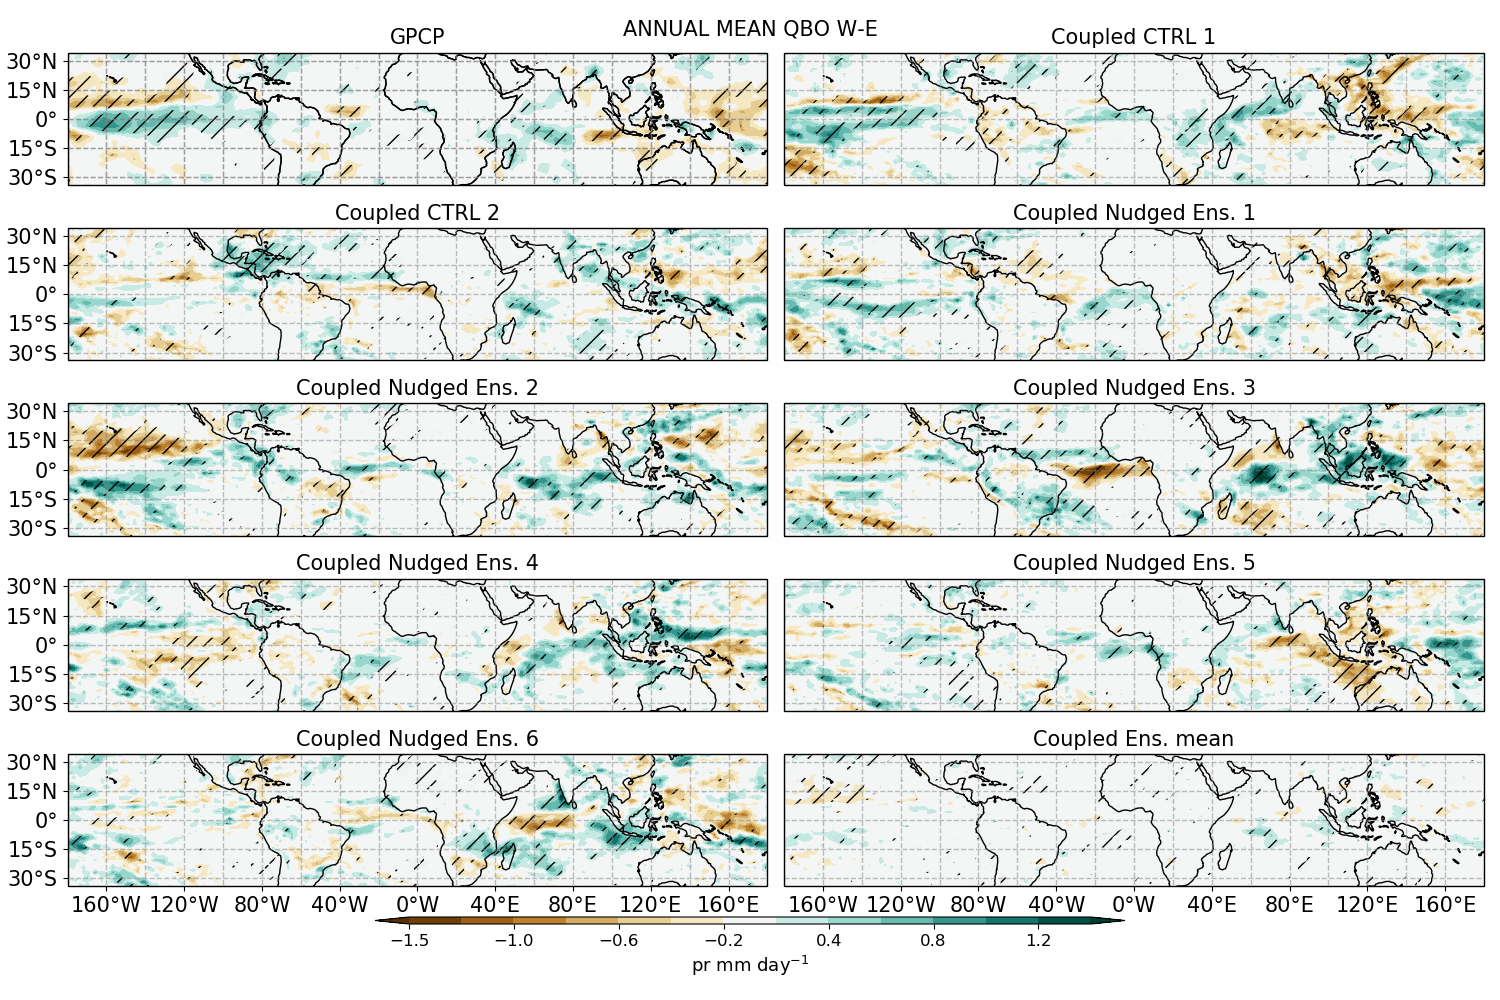
\includegraphics[width=\linewidth]{figures/pr_check_climqbowqboe.png}
%\caption[Precipitation response to the QBO in coupled nudged experiments]{ Annual mean precipitation QBO W-E differences in GPCP, Coupled Control, Coupled Nudged ensemble members and the Coupled Nudged ensemble mean. Hatching denotes significance to the 95\% confidence level according to a bootstrapping with replacement test.}
%\label{fig:pr_clim_coupled}
%\end{figure}
%
%
%The annual mean difference between QBO phases (Fig. \ref{fig:pr_clim_coupled}) in each coupled experiment reveals a strong variability of the precipitation response, suggesting an important role of long-term variability for these responses. 
%In particular, the control experiments show two significant responses: the first control experiment shows a significant El Niño-like response over the Central and Eastern Pacific Ocean, whereas the second control experiment shows a northward shift of the Atlantic ITCZ and a wetter Caribbean Sea.
%Precipitation differences in the Indian Ocean and continent are also significant in both of these two coupled experiments, even though the pattern and magnitude of the difference is not a close match, both simulations suggest a wetter western Indian Ocean and continent. 
%Note that these three responses found in the Coupled Control experiments in this setup were also observed over the longer GC3 N96 and N216-pi experiments, described previously in this chapter.
%
%
%
%The nudged experiments show various different responses (Fig. \ref{fig:pr_clim_coupled}), with several regions showing significant responses of one sign in one ensemble member and another, also significant, response of an opposite sign in a different ensemble just as in the SST differences of Figure \ref{fig:sst_clim_coupled}. In most ensemble members, the stronger responses are seen over the ocean rather than over land.
%The nudged ensemble mean shows regions with a significant response but the difference value in signficant regions is too small to be represented by the colorbar, indicating a weak response. 
%
%\begin{figure}[t!]
%\centering
% \noindent
% 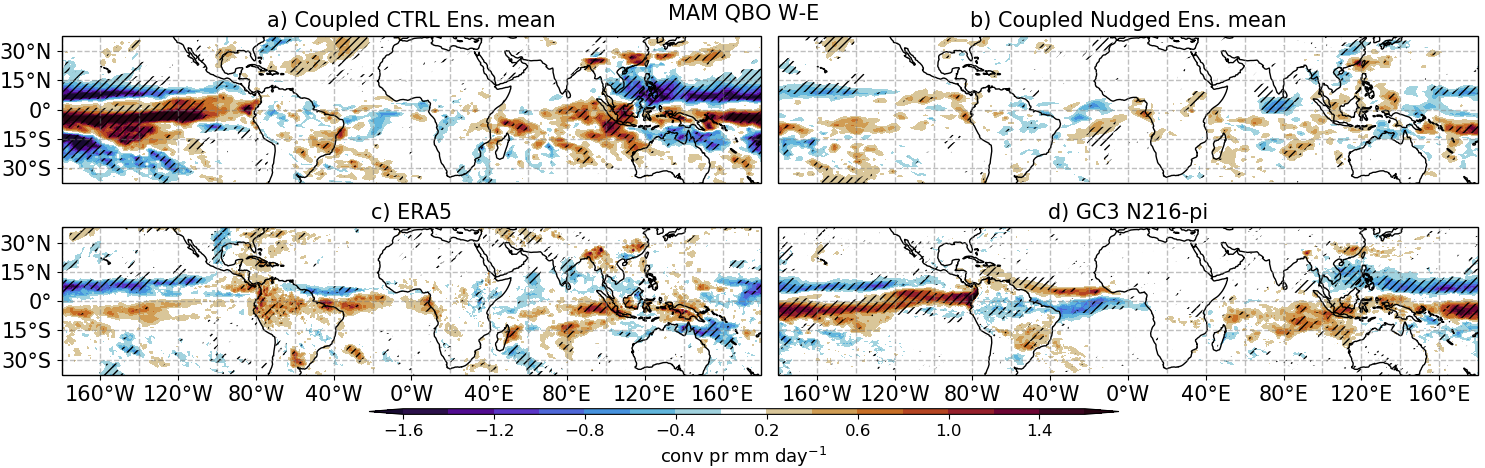
\includegraphics[width=\linewidth]{figures/conv_prseasonal_mamqbowqboe.png}
%\caption[ Convective precipitation response in MAM]{As in Fig. \ref{fig:sst_mam_coupled} but for convective precipitation.}
%\label{fig:conv_pr_mam_coupled}
%\end{figure}
%
%
%
%The differences in a specific season are also relatively weak in the ensemble mean of the nudged experiments. 
%For instance, in boreal spring, the differences in convective precipitation (Figure \ref{fig:conv_pr_mam_coupled}) show a wetter equatorial Pacific and a drier band at 10$^\circ$N during QBOWthan E in the control ensemble mean and CMIP6 experiments, whereas the nudged experiments only show the dry response. The Coupled Control ensemble mean and CMIP6 experiments also show agree on the sign and pattern of the response in the Western Pacific and Indian Ocean, characterized by dry anomalies in the Western Pacific ITCZ, the Philippines and the South China Sea, whereas wetter anomalies are observed in the Indian Ocean. 
%In contrast, the composite mean results in the nudged experiments show unsignificant responses in these above mentioned regions. 
%
%
%
%In other seasons, the control experiments also match the results of the CMIP6 experiments, whereas the nudged experiments show a weaker or no response. For example, in boreal summer (Fig. \ref{fig:conv_pr_jja_coupled}) the CMIP6 experiments and Coupled Control experiments show a northward shift of the Atlantic ITCZ, a wetter Caribbean Sea and Indian Oceans and a drier eastern Pacific. The nudged experiments are in reasonable agreement in the Indian Ocean, indicating wetter conditions during QBOWthan E.
%Similarly, the effects over the Indian Ocean in SON found for the CMIP6 experiments in section \ref{sq:cmip6_qbo}, are also seen in the Coupled Control experiments, but not in the nudged experiments (not shown).
%
%
%\begin{figure}[t!]
%\centering
% \noindent
% 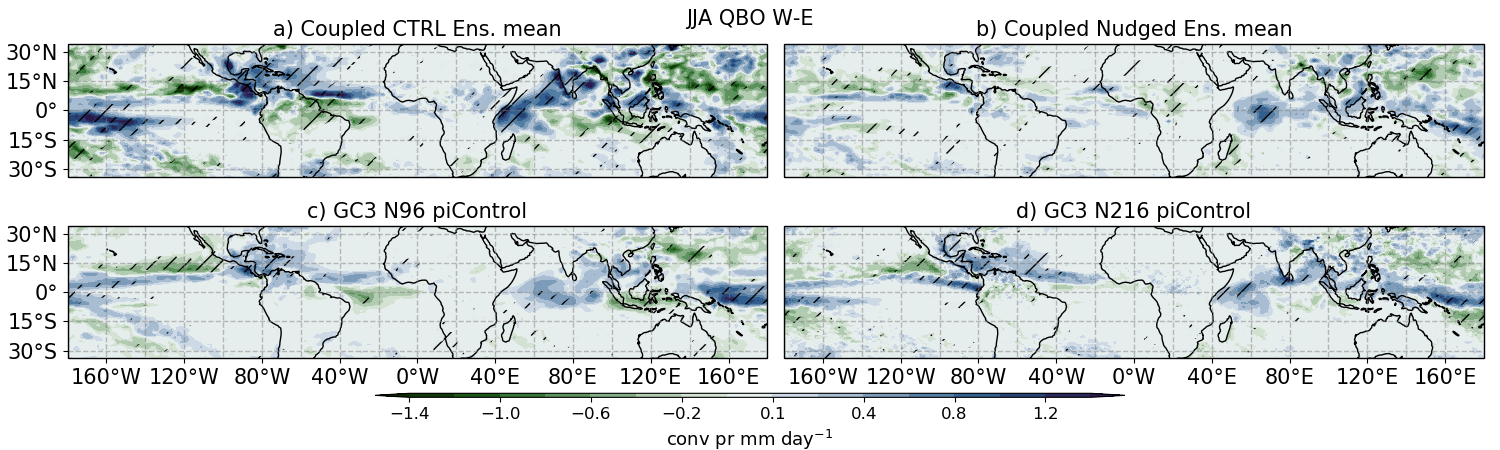
\includegraphics[width=\linewidth]{figures/conv_prseasonal_jjaqbowqboe.png}
%\caption[ Convective precipitation response in JJA]{As in Fig. \ref{fig:conv_pr_mam_coupled} but for JJA.}
%\label{fig:conv_pr_jja_coupled}
%\end{figure}
%
%The results of the precipitation response agree with the previous results that analysed the SST differences. There is no evidence that the nudged experiments result in a stronger surface response to the phase of the QBO, even though the UTLS temperature variability associated with the QBO has been increased and improved in the nudged experiments. 
%However, whether the mean state and variability of the tropical circulation has been modified could offer an explanation to these results.
%
%\subsubsection{Tropical circulation response and the IOD}
%
%\begin{figure}[t!]
%\centering
% \noindent
% 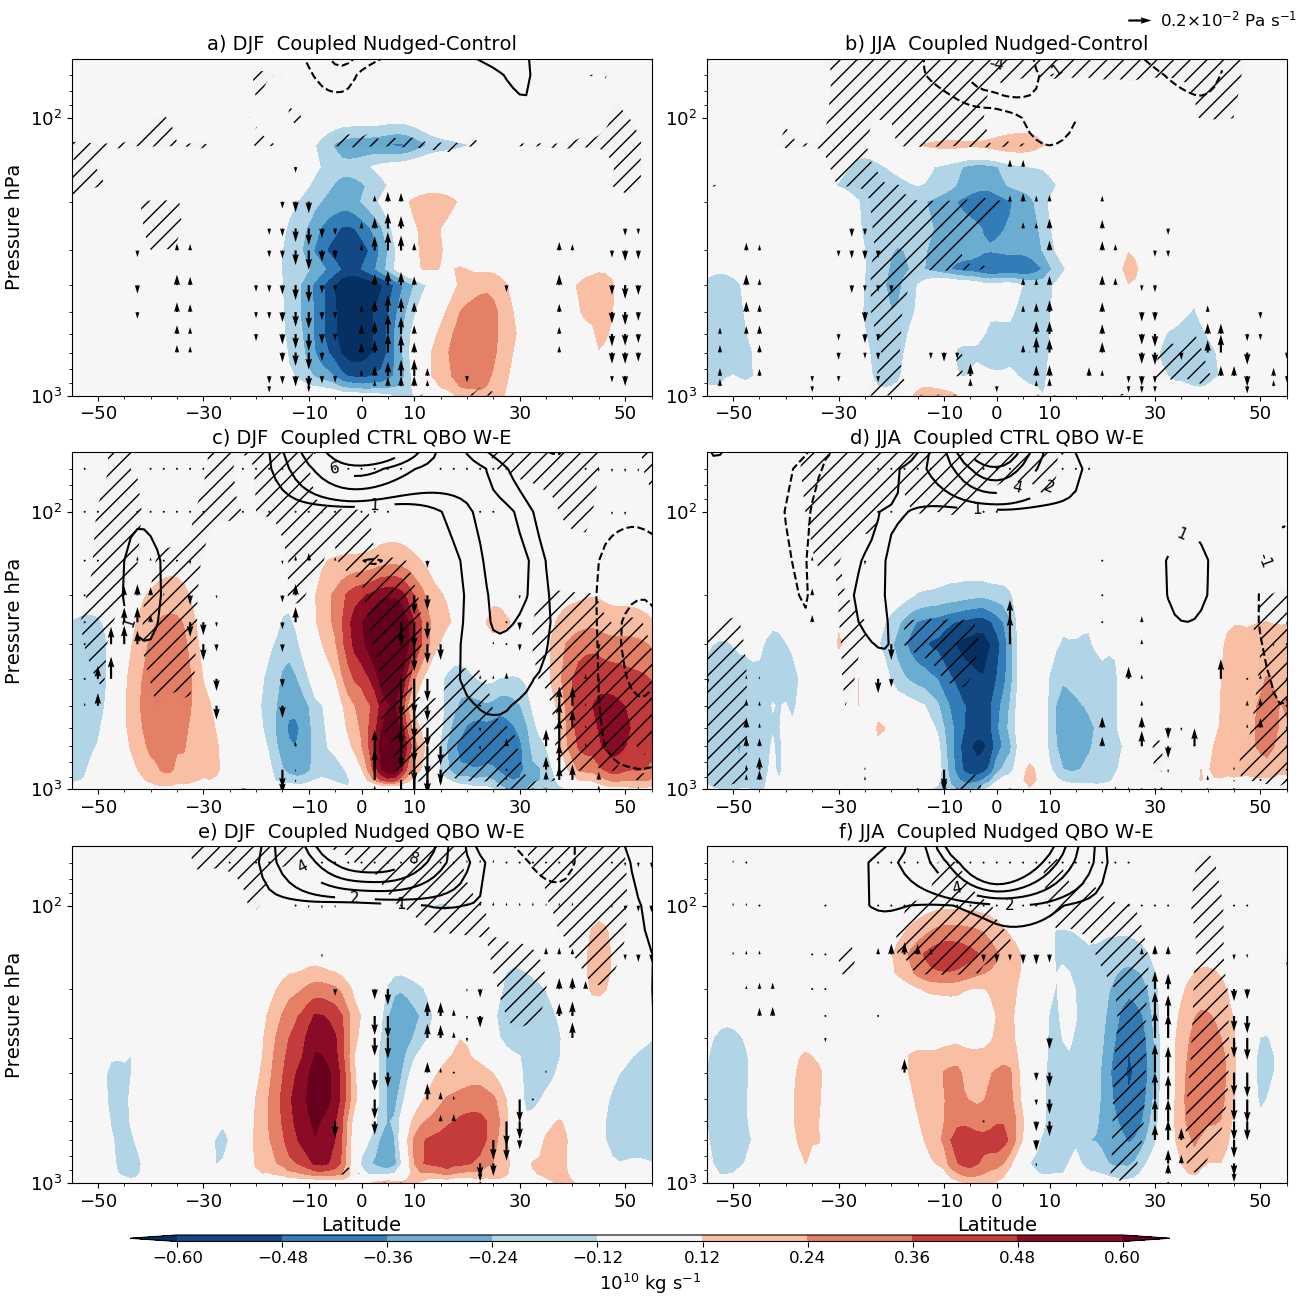
\includegraphics[width=\linewidth]{figures/suite_coupledhadley.png}
%\caption[Hadley circulation in coupled nudged experiments.]{Hadley circulation differences in meridional mass streamfunction (shading), zonal wind (contours) and vertical velocity (vectors). (a, b) show the seasonal mean differences between Nudged and Control coupled experiments in (a) DJF and (b) JJA. (c-f) show the QBO W-E differences for the (c-d) Control and (e-f) Nudged experiments for (c,e) DJF and (d,f) JJA. In all panels, hatching denotes significant differences in the streamfunction to the 95\% confidence level according to the bootstrapping method, whereas for the zonal wind and omega, only significant differences are shown.}
%\label{fig:hadley_coupled}
%\end{figure}
%
%The variability of the tropical circulation in the atmosphere-only experiments was found to be dominated by the SST forcing in the previous section. However, to the mean state of the upper-level branch of the Walker circulation was slightly different in the AMIP Nudged experiments compared to the Control. 
%To understand whether similar changes to the mean state or variability of the tropical circulation are observed in the coupled experiments, Figures \ref{fig:hadley_coupled} and \ref{fig:walker_coupled} show the impact of nudging on the mean state and variability of the Hadley and Walker circulations, respectively.
%
%The nudging appears to modify the mean state of the Hadley circulation in both DJF and JJA seasons (Figure \ref{fig:hadley_coupled}). Significant changes in the tropical UTLS streamfunction are observed in both seasons, and in DJF changes to the vertical velocity in the tropics suggest a strengthening of the Hadley cell when nudging is applied but very small changes are observed in JJA. 
%
%\begin{figure}[t!]
%\centering
% \noindent
% 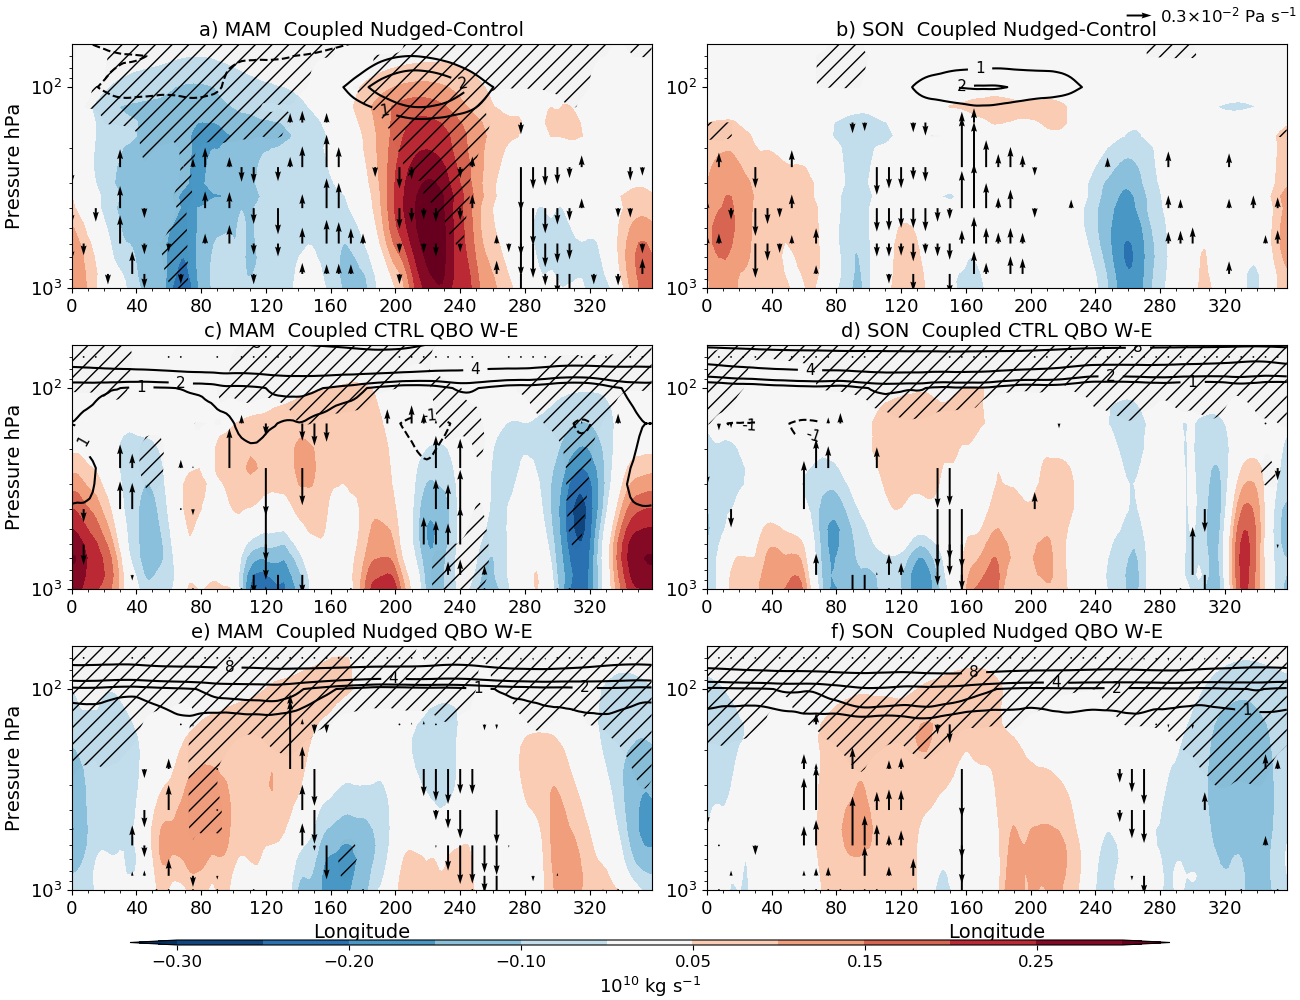
\includegraphics[width=\linewidth]{figures/suite_coupledwalker.png}
%\caption[Walker circulation in coupled nudged experiments.]{Walker circulation differences in zonal streamfunction (shading), zonal wind (contours) and vertical velocity (vectors). (a, b) show the seasonal mean differences between Nudged and Control coupled experiments in (a) MAM and (b) SON. (c-f) show the QBO W-E differences for the (c-d) Control and (e-f) Nudged experiments for (c,e) MAM and (d,f) SON. In all panels, hatching denotes significant differences in the streamfunction to the 95\% confidence level according to the bootstrapping method, whereas for the zonal wind and omega, only significant differences are shown.}
%\label{fig:walker_coupled}
%\end{figure}
%
%The difference QBO W-E in the tropospheric state of the Hadley cell in both seasons is considerably different between Nudged and Control experiments (Figs. \ref{fig:hadley_coupled}c-f). 
%In DJF, the Nudged ensemble-mean shows anomalous descent over the 10$^\circ$N latitude band and significantly higher values of the streamfunction at the equator extending into the lower troposphere. Similarly, the zonal wind in this season shows a positive anomaly extending as far down as 500 hPa at 20-30$^\circ$N, indicative of changes to the sub-tropical jet position and strength, documented previously \citep[e.g.][]{garfinkel2010}.
%
%Even though the Nudged experiments show stronger zonal wind anomalies in the equatorial stratosphere in both seasons, the response of the northern hemisphere subtropical jet is not observed, and the differences in the streamfunction and vertical velocity appear opposite to that of the Control experiments in DJF. 
%The same contrast is observed in JJA, with the Control and Nudged experiments exhibiting very different responses. Notably, the streamfunction and vertical velocity in the Nudged experiments in this season shows a dipole signal in the Northern Hemisphere with positive and negative anomalies indicating anomalous ascent at 30$^\circ$N and descent at 50$^\circ$N.
%
%The mean Walker circulation is also affected by the nudging (Fig. \ref{fig:walker_coupled}). As in the AMIP experiments, the upper-level zonal wind and streamfunction is modified by the nudging, only that in the coupled experiments, significant differences are observed in the lower troposphere over the Indian Ocean and the Eastern Pacific. 
%In the UTLS region above the Indian and Pacific Oceans, the nudging is forcing the zonal wind towards ERA5, thus reducing the biases in the model (see e.g. Figure \ref{fig:swalker}). In other words, not only biases in the variability of the zonal winds in the lower stratosphere are alleviated by the nudging but also the mean state of the upper-level branch of the Walker circulation. However, the latter may also mean that the variability of the Walker circulation is overconstrained when nudging is applied. 
%
%The response of the Walker circulation to the QBO is different in nudged versus control experiments (Fig. \ref{fig:walker_coupled}c-f). While in MAM, the control results suggest a weaker state of the Walker circulation or an El Niño-like pattern with anomalous ascent in the Eastern Pacific, the nudged simulations show the opposite. 
%In turn, in SON, while the control experiments show anomalous ascent in the western Indian Ocean, the nudged experiments show ascent over the eastern Indian Ocean. 
%
%The nudging appears to modify the mean state and variability of the tropical circulation to a certain extent. However, the differences shown in Figures \ref{fig:hadley_coupled} and \ref{fig:walker_coupled} are relatively small compared to the climatological values,  but clearly some of these differences are still significant. 
%
%Results in a previous section demonstrated that in the CMIP6 pre-industrial control experiments a statistically significant relationship is found between the IOD and ENSO, and the QBO (Fig. \ref{fig:iod_barplot}). 
%Positive events of the IOD and ENSO are more commonly found during QBOW than E, and a convective precipitation index of the IOD and the SST EN3.4 index are also positive during QBOW and negative during QBOE. 
%Figure \ref{fig:iod_suites} revisits these relationships in the coupled experiments. 
%
%\begin{figure}[t!]
%\centering
% \noindent
% 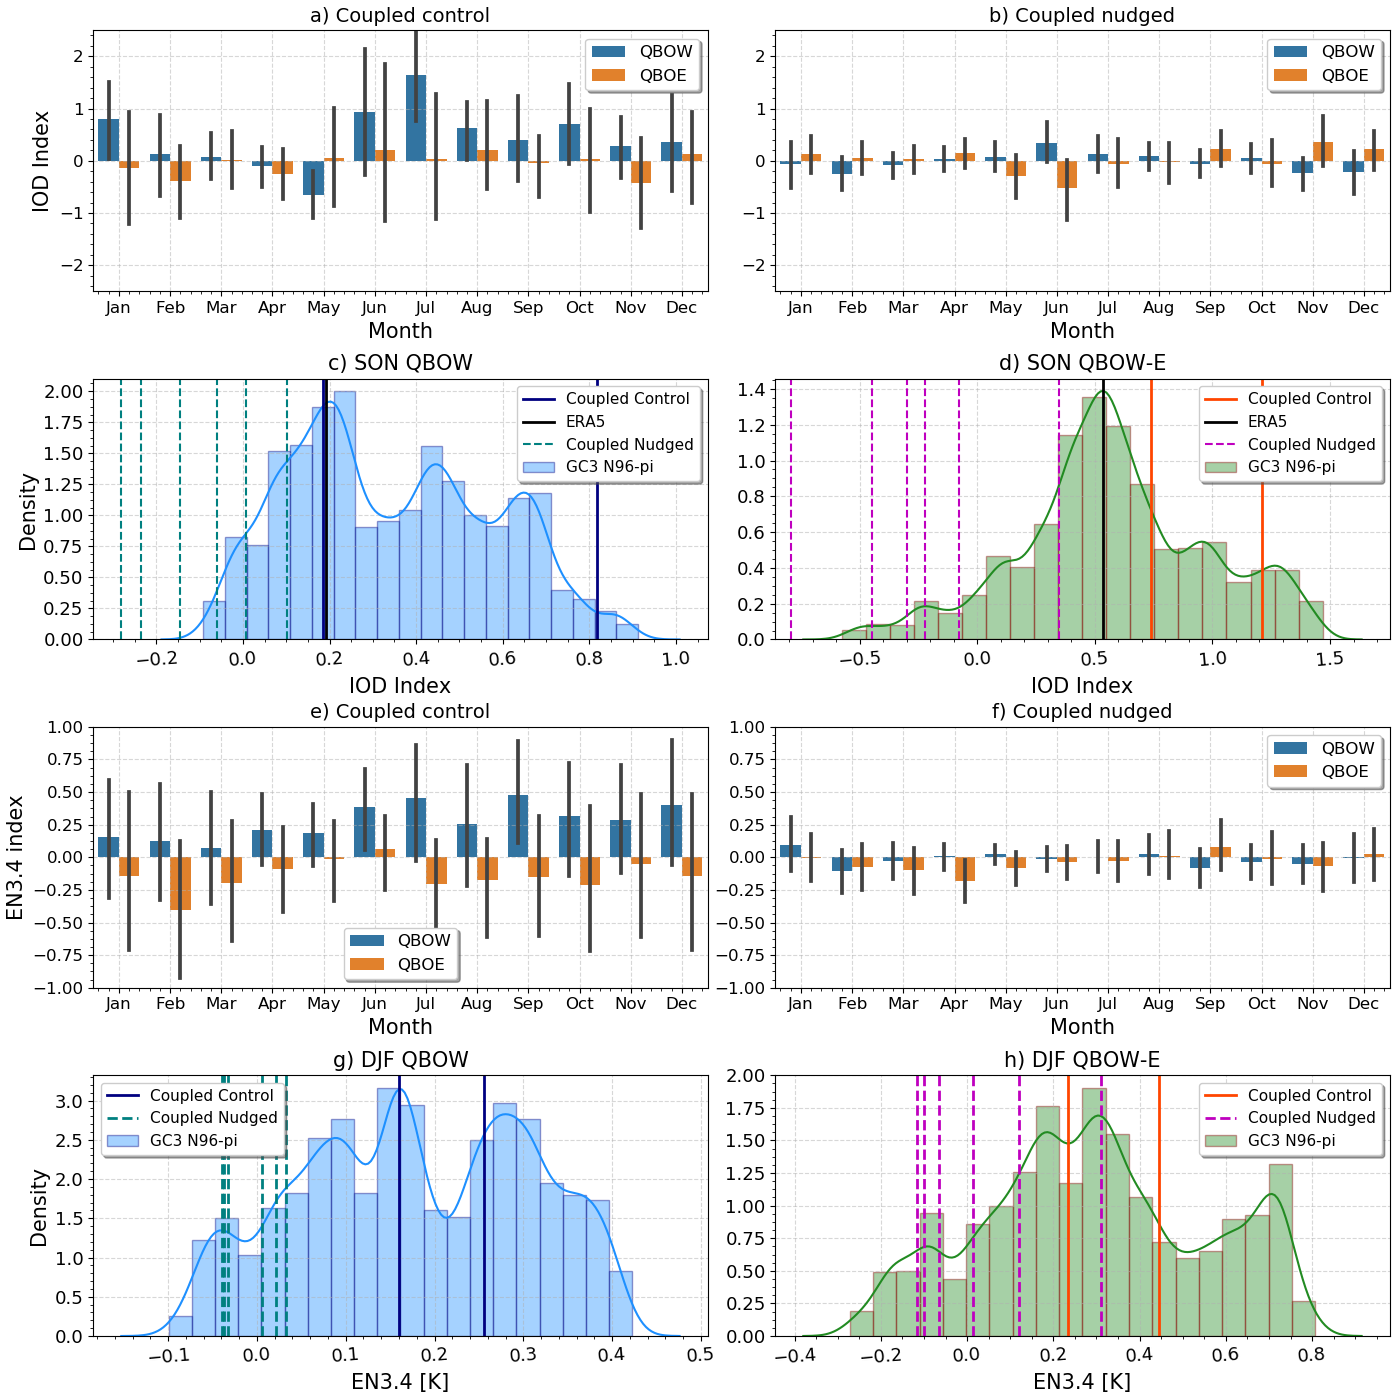
\includegraphics[width=\linewidth]{figures/iod_suites.png}
%\caption[IOD and ENSO indices in nudged versus control experiments]{(a, b) Monthly-mean IOD convective precipitation index [mm day$^{-1}$] in coupled (a) control and (b) nudged ensemble-means separated by QBO phase. (c, d) Probability density functions (PDFs) of the IOD convective precipitation index for (c) the mean SON during QBOW months and (d) the SON difference between QBO W-E. The PDF is obtained from the 500 yrs of the GC3 N96-pi by bootstrapping 10,000 times into 35-yr periods and obtaining the averages and differences in each subsample. The mean indices for the Coupled Control and Nudged experiments, as well as for ERA5 are also shown. (e, f) Monthly-mean EN3.4 index [K] in the ensemble mean (e) Coupled control and (f) Coupled Nudged simulations separated by QBO phase.   }
%\label{fig:iod_suites}
%\end{figure}
%
%The mean IOD index is positive during QBOW and negative during QBOE in the Coupled Control ensemble in boreal fall and early winter (Fig. \ref{fig:iod_suites}a), in agreement with results from the CMIP6 experiments. In contrast, the mean IOD index is close to zero in the Coupled Nudged ensemble without any clear relationship between the index and the QBO phase in any month (Fig. \ref{fig:iod_suites}b). 
%These results suggest that no consistent relationship is found across the six ensemble members where nudging was applied in the simulation. 
%However, these results may simple be due to sampling of the ocean-atmosphere state used for the nudged experiments, in other words, possibly due to decadal variability in the GC3.1 configuration.
%
%For that reason, the CMIP6 GC3 N96-pi is used to investigate whether the results of the Nudged and Control experiments are also seen in periods of similar length in that long 500 yr simulation. While this comparison is not perfect due to differences in ocean resolution and forcing, the model setup and parametrisations, and atmospheric resolution is otherwise the same between GC3 N96-pi and these experiments. 
%The simulation is repeatedly sampled at random for 35 yr continous periods, and the SON IOD index is computed each time to construct a probability distribution.  
%
%Figure \ref{fig:iod_suites}c shows that the IOD index during QBOW in GC3 N96-pi is more frequently positive, as shown in the previous section, but in some 35-yr periods a negative mean index during QBOW can be observed in this simulation. The two Coupled Control simulations and ERA5 show a positive mean IOD index during QBOW whereas four out of the six Coupled Nudged simulations show a negative index. 
%
%The previous section showed not only that positive IOD indices and events are more frequent during QBOW, but also that the opposite is true for QBOE. Figure \ref{fig:iod_suites}d  shows that the difference in the IOD index during SON between the two QBO phases is most frequently positive in GC3 N96-pi.  
%Results from ERA5 and the two Coupled Control simulations also show a positive difference of 0.6 mm day$^{-1}$ for the reanalysis and up to 1.3 mm day$^{-1}$ for one of the control simulations. 
%In contrast, the nudged experiments are found to the left of the mean of the PDF of GC3 N96-pi and the mean of the Control experiments, with a mean negative values in most ensemble members the mean of one member is found to the leftmost end of the PDF. 
%
%Finally, the ENSO index is found to be positive in the Control experiments but no robust relationship is found in the Nudged experiments. As with the CMIP6 experiments, the Coupled Control EN3.4 index is positive during QBOW and negative during QBOE throughout most of the year. However, there seems to be no relation between the QBO and the EN3.4 index in the nudged experiments. 
%Overall, these results suggest that the relationships between the QBO and the IOD and ENSO observed in the CMIP6 or Control experiments are not found in the Nudged experiments, which show little-to-no relationship between these two indices and the QBO phase.
%
%\section{Summary and discussion}
%
%This chapter investigates the tropical route of QBO teleconnections in the global climate models of the MOHC.
%In addition to multiple lines of observational and modelling evidence that suggest an influence of the QBO over tropical convective phenomena, results from Chapter \ref{ch:4-ams} showed that the impact of ENSO on the Walker circulation and associated teleconnections was sensitive to the phase of the QBO in the CMIP6 experiments of the MOHC and this chapter follows up on that evidence. 
%The first part of the chapter analyses CMIP6 experiments that reasonably simulate the QBO features, and the second part of the chapter describes and reports the results of simulations realized with MOHC models in which the equatorial stratosphere was relaxed towards an observed state.
%
% First, the chapter describes the annual and seasonal mean surface response of precipitation to the two phases of the QBO in the CMIP6 pre-industrial control experiments: UKESM-pi, GC3 N96-pi, GC3 N216-pi.  
%Results in the models generally agree with the results documented in observational studies \citep{liess2012,gray2018} and with the observational and reanalysis datasets employed throughout this thesis. In particular, the most robust impacts are observed over the ocean, particularly over two coupled ocean-atmosphere phenomena: the East Pacific and Atlantic ITCZ and the IOD. 
%
%The position of the East Pacific and Atlantic ITCZs is significantly different between the two phases of the QBO in the three experiments; however, the season of strongest influence varies for each model. 
%For example, the southward displacement of the East Pacific ITCZ in QBOW compared to QBOE phases  \citep[as previously reported, e.g., by][]{gray2018} is confirmed but in GC3 N216-pi this shift of the ITCZ is strongest in MAM whereas in GC3 N96-pi the most pronounced shift is in the DJF season. 
%The position of the Atlantic ITCZ is found northward during QBOW than during QBOE periods in all the simulations, but the strongest impact is found during late boreal spring and early summer in UKESM-pi. 
%
%For most land-monsoon regions, little evidence was found of robust impacts on the local summer monsoon precipitation associated with the QBO. For example,  the South American monsoon region exhibited different responses in eastern Brazil than in the southernmost part of the monsoon. The surface response over land also varied notably from model to model.
%One hypothesis for the lack of a robust signal over land is the differences in the representation of the monsoon dynamics and feedbacks between the three models UKESM-pi, GC3 N96-pi, GC3 N216-pi that may represent the land-surface processes and moisture transport differently, so that any grid-scale impact of the QBO on the convective profile may produce different dynamic responses in the lower troposphere. 
%
%The influence of the QBO over the Indian and Pacific Oceans was confirmed through multi-variate regression analysis, suggesting an independent effect of the QBO from ENSO in these ocean basins. 
%However, the QBO-related differences over the Atlantic and East Pacific ITCZ appear to also depend on the phase of ENSO, suggesting a non-linear interaction between the ITCZs, ENSO and the QBO which may be confounded when using regression analysis.  
% The observed relationship between the QBO and ENSO is confirmed in this chapter in the CMIP6 experiments, as more frequently El Niño events appear during QBOW than during QBOE and the opposite for La Niña. 
% 
% A zonal gradient of convective precipitation in the Indian Ocean appeared in all the simulations during SON. 
% This zonal gradient was further diagnosed through an index that was found to be significantly sensitive to the QBO  phase, the index was found to be positive during QBOW and negative during QBOE, indicative of wetter conditions in the western Indian Ocean than in the eastern  Indian Ocean during QBOW and the opposite during QBOE. 
% 
% The hypothesis that the QBO may influence the mean-state of the Walker circulation suggested by previous observational studies to explain zonally asymmetric responses \citep[e.g.][]{collimore2003,liess2012} is confirmed as the Walker circulation varies up to 10\% between QBO phase, even when the effect of ENSO events is taken into account. 
% Specifically, the Walker circulation is found to be weaker during QBOW than during QBOE. In DJF, this anomaly of the overturning circulation in the Pacific is likely linked to the East Pacific ITCZ shifts, and in SON, the changes to the overturning are likely linked to the ascending and descending motions in the Indian Ocean, however the direction of causality could not be addressed in this part of the chapter, which leads into the second part of the chapter.
% 
%
%The MOHC models exhibit a key bias in the lower-stratosphere characterised by a weaker QBO amplitude in zonal wind and temperature in the lower stratosphere compared to the observed QBO. This bias is key because according to the literature the mechanism through which the QBO influences the tropics is the vertical temperature gradient in the UTLS \citep{liess2012,nie2015,lee2018}. Since models simulate a weaker than observed temperature difference between the two QBO phases, nudging or relaxation experiments have been proposed \citep{lee2018} to alleviate this bias. 
%
%For that reason, simulations with the UM using the HadGEM3 GC3.1 configuration were performed using a relaxation of the zonal winds above 90 hPa towards reanalysis. 
%The main hypothesis of these experiments being that improving the simulation of the QBO temperature signal would produce a stronger response in the tropical circulation and surface precipitation to the phase of the QBO. 
%
